% ============================================================
%  Capítulo 5 — Diseño
%  TT 2026-B066 | ESCOM-IPN
%  Frausto Robles Ángel Ali · Rodríguez Verdín Sandoval Vanesa
% ============================================================

\chapter{Diseño}

Este capítulo describe las decisiones de diseño del sistema: cómo están organizados
sus módulos, cómo se estructura la base de datos, cómo se comunican los componentes
a través de la API REST, y cómo se ve la interfaz desde la perspectiva del investigador.
También incluye el diseño del pipeline de análisis conductual: el flujo de procesamiento
de video, la estrategia de separación por sujeto y la arquitectura del clasificador.

Los diagramas de este capítulo siguen la notación \textit{Unified Modeling Language}
(UML) versión~2.5.1, especificada por el \textit{Object Management Group}
(OMG) \cite{omg_uml}, organismo que gestiona y publica las actualizaciones del
estándar desde 1997. UML está también adoptado como estándar internacional bajo
ISO/IEC~19501:2005 \cite{iso19501}, que define la notación y el metamodelo para
diagramas de casos de uso, secuencias y clases. La estructura arquitectónica del
sistema se documenta conforme a ISO/IEC/IEEE~42010:2011 \cite{iso42010}, norma que
establece cómo describir una arquitectura de software mediante múltiples vistas
---estructural, de comportamiento y de despliegue--- que atienden las preocupaciones
de los distintos actores del sistema.

La decisión de diseño más importante fue separar el worker del backend en un proceso
independiente. La opción más simple habría sido ejecutar el pipeline dentro del mismo
servidor Flask, pero eso significa bloquear todas las peticiones HTTP mientras un video
de 20 minutos se procesa. El worker resuelve ese problema a costa de mayor complejidad
en el despliegue: hace falta una cola de tareas, un proceso adicional y comunicación
entre procesos. Esa complejidad extra está justificada porque el laboratorio puede
tener varios análisis en cola al mismo tiempo.

% -----------------------------------------------------------
\section{Arquitectura general del sistema}
% -----------------------------------------------------------

El sistema tiene una arquitectura cliente-servidor de tres capas separadas en
contenedores Docker independientes: frontend, backend y base de datos. Un cuarto
contenedor ---el worker--- ejecuta el pipeline de análisis de forma asíncrona, sin
bloquear al servidor web mientras procesa los videos.

La Figura~\ref{fig:arquitectura_software} muestra qué tecnología reside en cada
contenedor y cómo se comunican entre sí. Se distinguen cuatro grupos: la capa de
presentación (React.js + Vite), la lógica de negocio (Flask + SQLAlchemy), el
procesamiento asíncrono (OpenCV, scikit-learn y PyTorch) y la capa de datos
(PostgreSQL, sistema de archivos y volumen de modelos entrenados). El archivo del
clasificador de conducta reside en un volumen Docker dedicado que el worker monta al
arrancar el contenedor.

\begin{figure}[H]
\centering
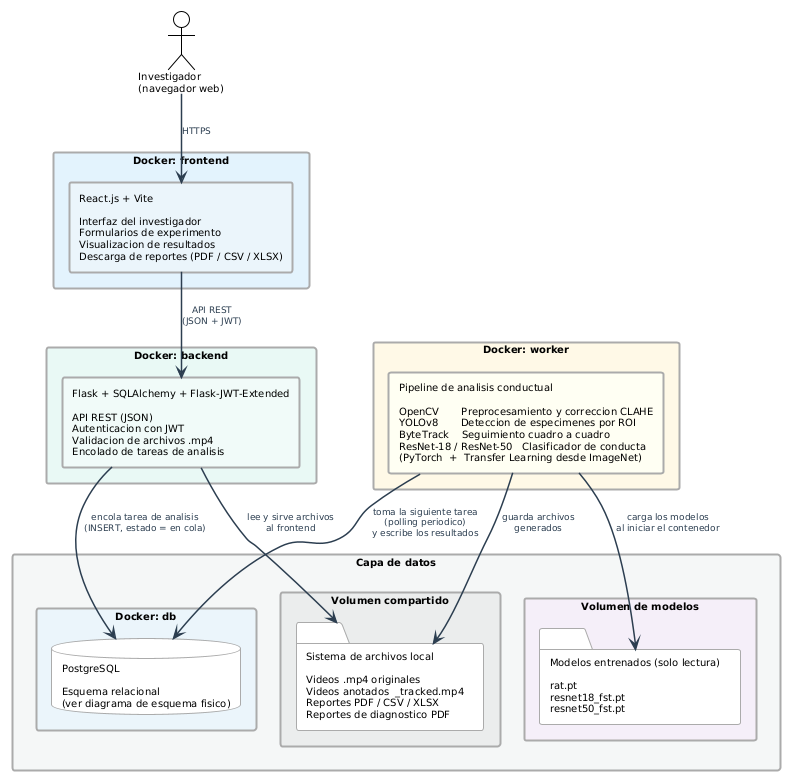
\includegraphics[width=\textwidth]{figures/mermaid/arquitectura_software}
\caption{Arquitectura de software por capas tecnológicas [autoría propia].}
\label{fig:arquitectura_software}
\end{figure}

Las responsabilidades de cada componente son:

\begin{itemize}
  \item \textbf{Frontend (React.js + Vite):} corre en el navegador del investigador.
        Se comunica con el backend exclusivamente mediante la API REST usando JSON.
        No tiene acceso directo a la base de datos ni al sistema de archivos del
        servidor.

  \item \textbf{Backend (Flask):} expone la API REST, gestiona la autenticación con
        JWT, valida los archivos subidos, encola las tareas de análisis y devuelve
        los resultados al frontend. Usa SQLAlchemy como ORM para interactuar con
        PostgreSQL.

  \item \textbf{Worker (Python):} proceso independiente que consume tareas de la
        cola, ejecuta el pipeline completo de análisis (preprocesamiento, localización
        de los cilindros y clasificación) y escribe los resultados en la base de datos.
        Al correr en un proceso separado, el servidor web sigue respondiendo a
        otras peticiones mientras el video se procesa.

        La cola de tareas no es un servicio aparte: es la propia tabla
        \texttt{ANALISIS}. Cuando se sube un video válido, el backend crea un
        registro con estado «en cola». El worker obtiene las tareas mediante
        \textit{polling} (consulta periódica): cada cierto tiempo consulta esa tabla,
        toma un análisis en cola, lo pasa a «procesando» y, al terminar, a
        «completado» o «error». Se eligió este enfoque en lugar de un sistema de
        colas de mensajes dedicado (como Celery con RabbitMQ o Redis) porque evita
        un contenedor y una dependencia más; con el volumen del laboratorio, de
        hasta cuatro análisis en un mismo período, la base de datos basta como cola.

  \item \textbf{Base de datos (PostgreSQL):} almacena usuarios, experimentos,
        sesiones de video, resultados por espécimen y conducta, y reportes generados.
        Los archivos de video se guardan en el sistema de archivos del servidor, no
        en la base de datos.
\end{itemize}

La separación en contenedores cumple con el atributo de portabilidad de la
ISO/IEC/IEEE~12207:2017 \cite{iso12207}: el sistema puede desplegarse en cualquier
equipo con Docker instalado sin dependencias adicionales. La separación entre worker
y backend también satisface el RF-12 y el RF-15 (análisis automático en segundo plano) y permite
escalar el número de workers de forma independiente si el volumen de análisis aumenta.

La Figura~\ref{fig:flujo_sistema} muestra el flujo funcional del sistema: cómo
transita el video desde la carga hasta la generación de resultados, y cómo el ciclo
de entrenamiento del modelo ---anotación experta, dataset y entrenamiento--- alimenta
al clasificador de conducta.

\begin{figure}[H]
\centering
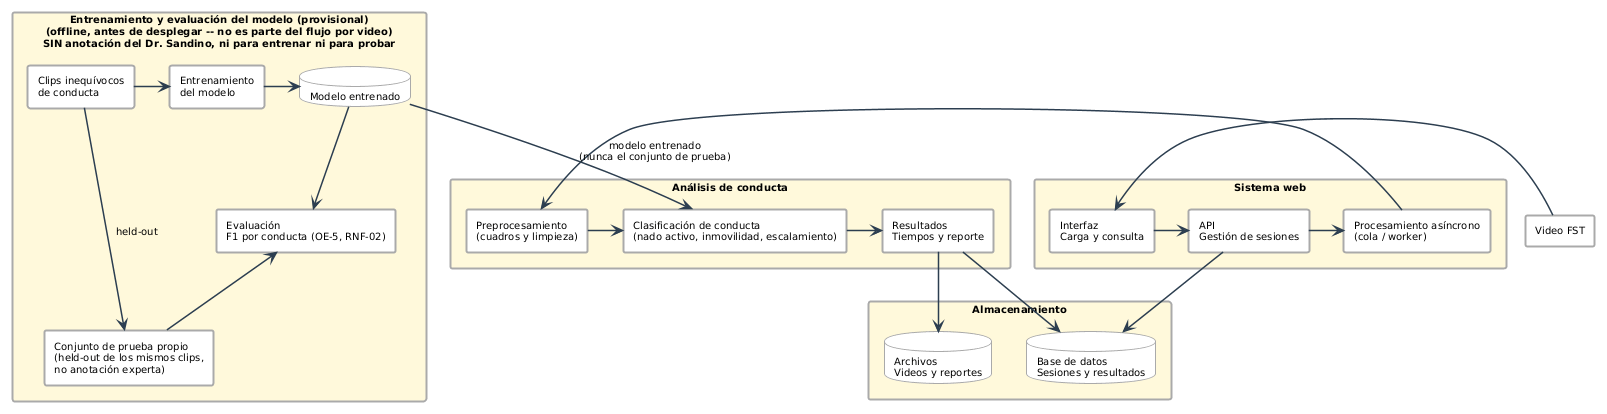
\includegraphics[width=\textwidth]{figures/mermaid/flujo_general}
\caption{Diagrama de flujo del sistema [autoría propia].}
\label{fig:flujo_sistema}
\end{figure}

% -----------------------------------------------------------
\section{Diseño del pipeline de análisis conductual}
% -----------------------------------------------------------

El pipeline recibe un video del FST, analiza solo sus primeros 300 segundos y produce
como salida los tiempos totales de cada conducta por espécimen y el desglose por minuto. Sigue el patrón arquitectónico de
tubería y filtro (\textit{pipe and filter}) \cite{sommerville2011}: cada módulo es
un filtro discreto que transforma los datos y los pasa al siguiente. Está organizado
en cuatro módulos secuenciales: preprocesamiento, localización de los cilindros,
clasificación de conducta y generación de resultados. La Figura~\ref{fig:pipeline}
muestra el flujo completo con las tecnologías de cada módulo.

\begin{figure}[H]
\centering
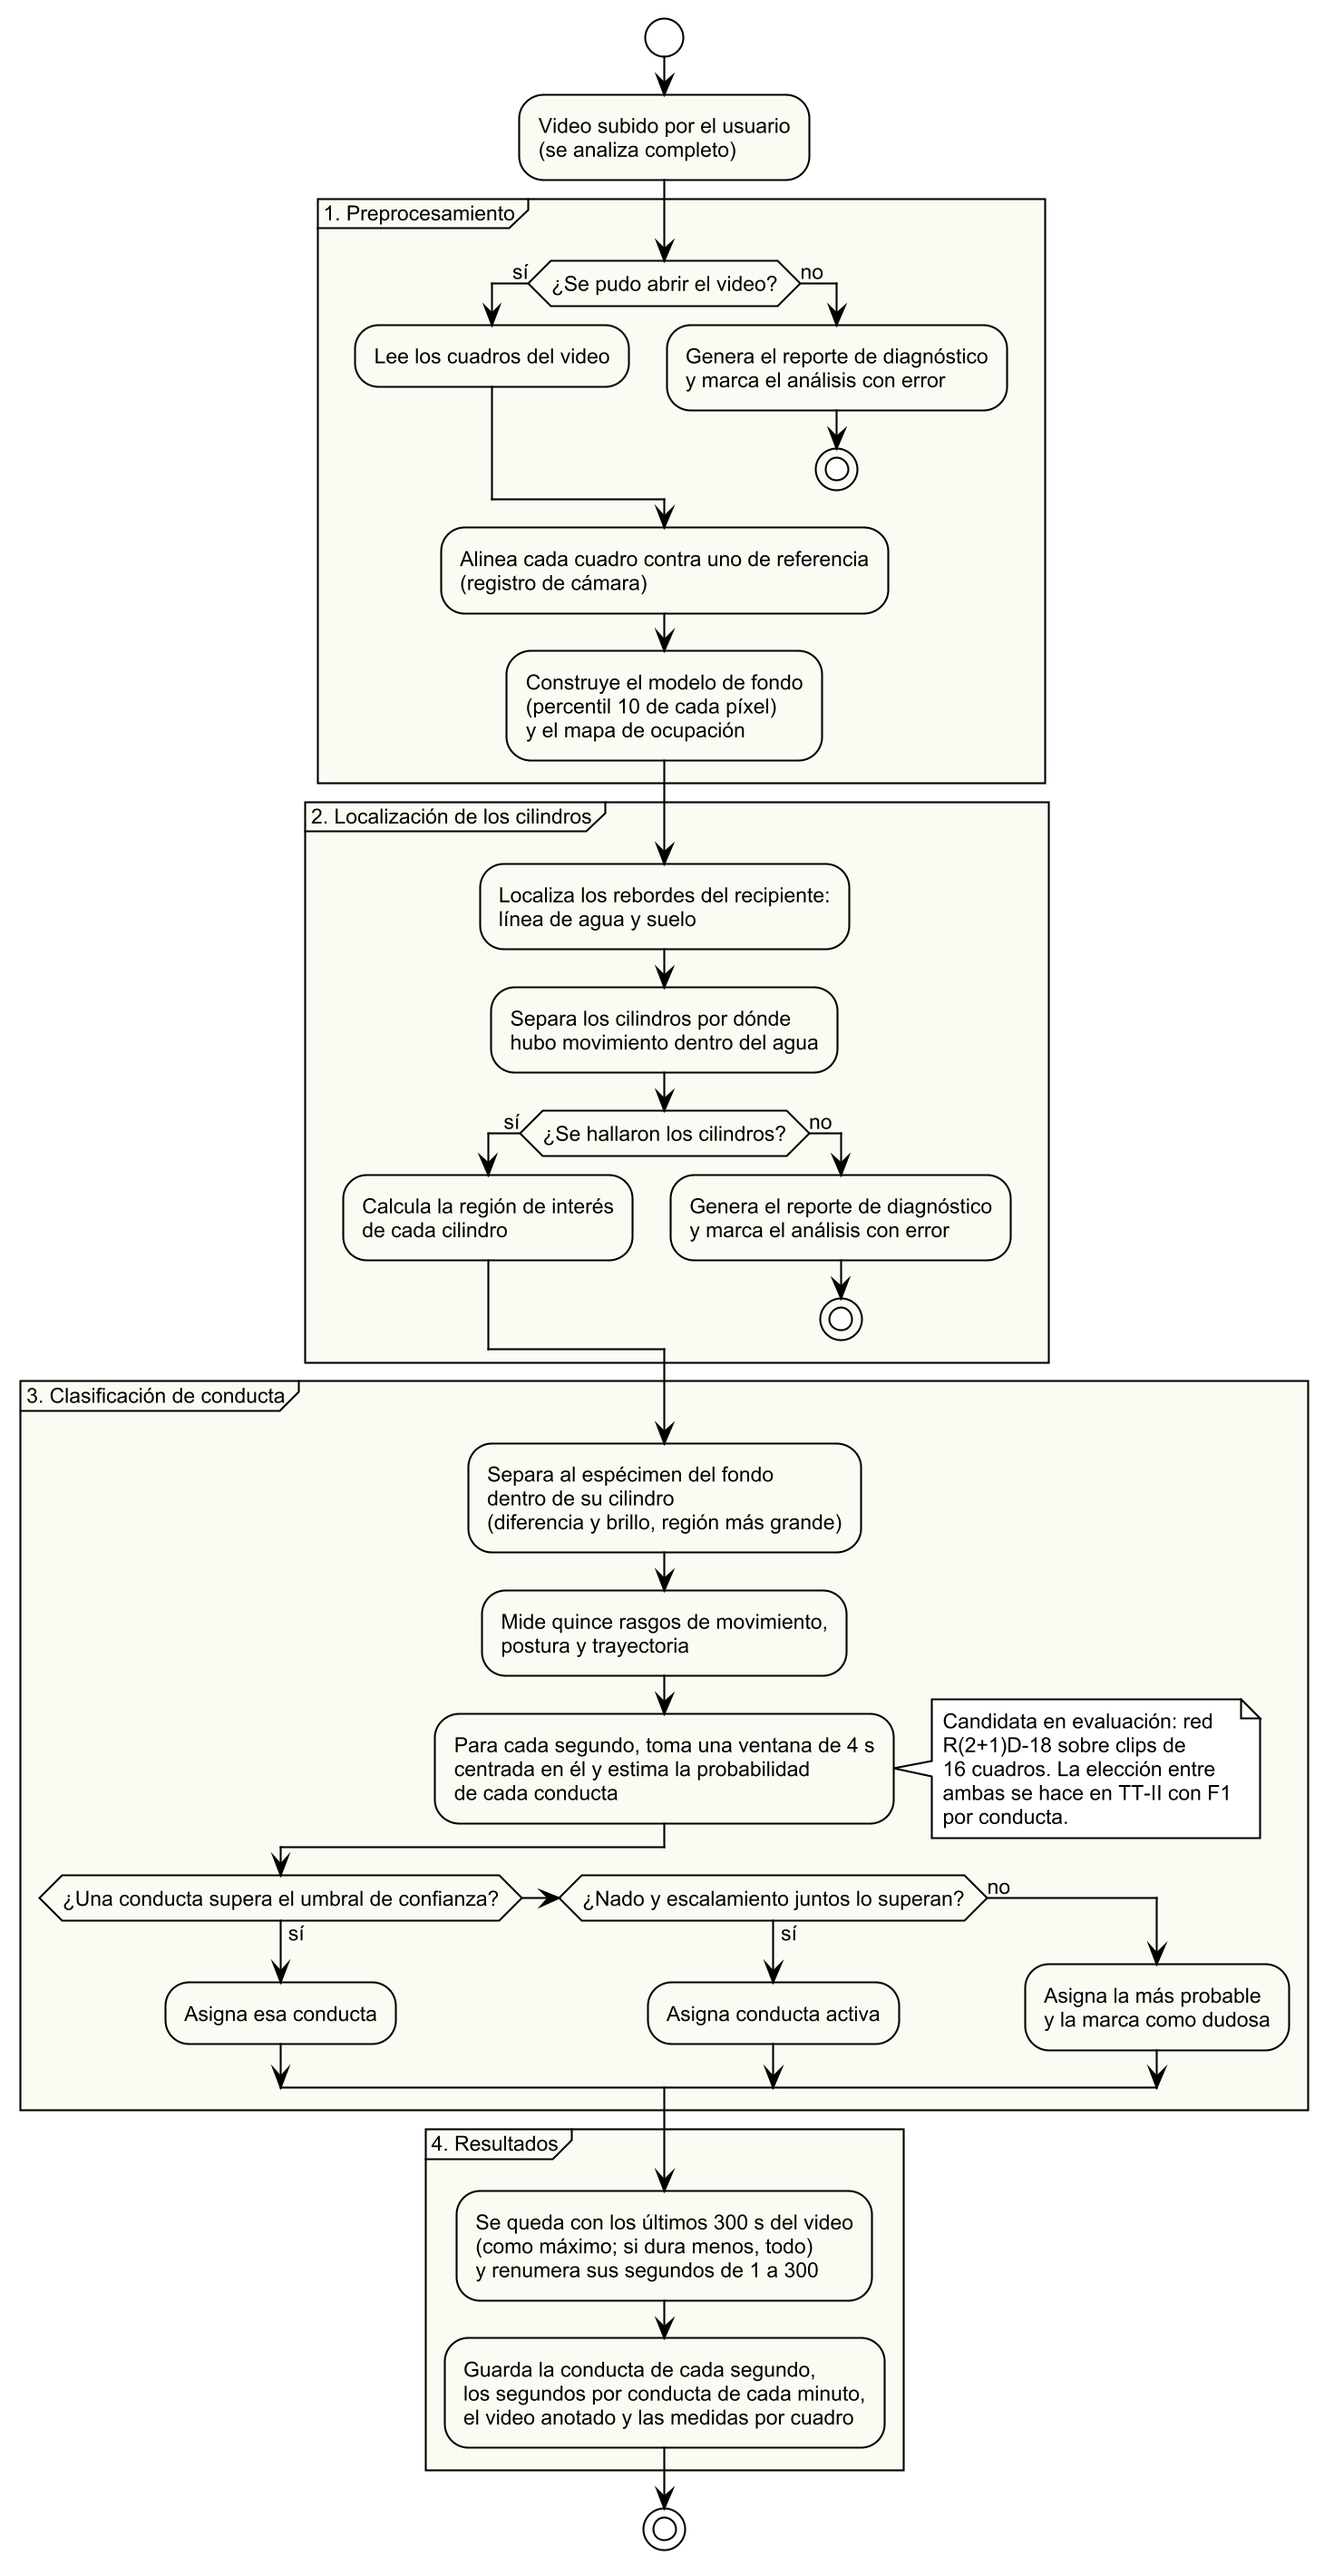
\includegraphics[width=\textwidth, height=0.85\textheight, keepaspectratio]{figures/mermaid/pipeline}
\caption{Diagrama de flujo del pipeline de análisis conductual [autoría propia].}
\label{fig:pipeline}
\end{figure}

\subsection{Módulo 1: Preprocesamiento}

El preprocesamiento usa \textbf{OpenCV VideoCapture} para decodificar el video
cuadro a cuadro. Primero alinea cada cuadro contra uno de referencia
(\textbf{registro de cámara}), para que un movimiento de la cámara no se confunda
con movimiento del espécimen. Después construye un \textbf{modelo de fondo}: la
imagen del aparato sin especímenes. Si el contraste promedio cae por debajo del umbral mínimo, se
aplica \textbf{CLAHE} (\textit{Contrast Limited Adaptive Histogram Equalization})
\cite{bradski2000} para normalizarlo. Si tras la corrección no se logran encontrar
los cilindros, el pipeline se detiene y genera un reporte de diagnóstico (ver RN-11).

\subsection{Módulo 2: Localización de los cilindros}

Sobre el modelo de fondo, el sistema localiza los bordes del recipiente, la
\textbf{línea de agua} y el suelo, y separa los cilindros midiendo dónde hay
movimiento dentro de la franja de agua. Para cada cilindro calcula una
\textbf{región de interés} (ROI) que delimita el área de análisis de cada espécimen.
Ninguna medida se escribe a mano: el sistema las deduce de cada video, así que
funciona con grabaciones de distintos días, encuadres y resoluciones.

Cada cilindro contiene un solo espécimen, así que no hace falta seguirlo de un
cuadro a otro con un algoritmo de seguimiento: lo que se mueve dentro de un
cilindro es su espécimen.

\subsection{Módulo 3: Clasificación de conducta}

La clasificación trabaja sobre el cilindro de cada espécimen y se basa en
aprendizaje supervisado. Se construye en dos partes: un clasificador sobre rasgos
medidos, que ya funciona y que además sirve para etiquetar el conjunto de
entrenamiento, y una red neuronal convolucional que se compara contra él y que
sigue en desarrollo.

\paragraph{Rasgos del espécimen.} Sobre la imagen estabilizada y con el espécimen
separado del fondo, el sistema mide quince rasgos que describen su movimiento (la
energía de movimiento medida solo dentro del cuerpo, para que el oleaje del agua no
la sature), su postura (verticalidad, alargamiento y área) y su trayectoria
(recorrido, amplitud y cuadrantes del cilindro que cruza). Las distancias se
expresan en largos de cuerpo y los tiempos en segundos: así, dos videos grabados
con encuadres distintos producen números comparables y el clasificador aprende la
conducta y no el encuadre.

\paragraph{Clasificador sobre rasgos.} Un clasificador de \textit{gradient
boosting} (potenciación del gradiente) sobre árboles de decisión
\cite{friedman2001}, en la variante por histogramas que implementa scikit-learn
como \texttt{HistGradientBoostingClassifier} \cite{pedregosa2011,ke2017}, recibe
los quince rasgos y estima la probabilidad de nado activo, inmovilidad y
escalamiento. La conducta se decide con una regla de tres pasos:

\begin{enumerate}
  \item Si una conducta supera el umbral de confianza, se asigna esa conducta.
  \item Si ninguna lo supera, pero la suma de nado activo y escalamiento sí, se
        asigna \textit{conducta activa}: el espécimen no está inmóvil, pero el
        clasificador no decide entre las dos conductas activas (ver RN-13).
  \item Si tampoco, se asigna la conducta más probable y el resultado se marca
        como dudoso para que la revisión humana lo atienda primero.
\end{enumerate}

\paragraph{Decisión segundo a segundo.} Para decidir el segundo $k$, el sistema
mide los rasgos en una ventana de 4~s centrada en él (desde 1.5~s antes hasta
2.5~s después) y aplica el clasificador. La ventana avanza un segundo a la vez,
así que cada segundo tiene su propia decisión y aparecen conductas breves, de unos
2~s, que una decisión por bloques de 5~s esconde. Una ventana más corta vería
conductas más breves, pero mediría con muy pocos datos; 4~s es el punto de
equilibrio. El segundo es la unidad con la que el sistema registra las conductas;
no se aplica una duración mínima de episodio (ver RF-18 y
sec.~\ref{sec:umbrales}). Al agrupar los segundos de cada bloque de 5~s y tomar la
conducta mayoritaria, el resultado se compara directamente con el análisis manual
por bloques.

\paragraph{Conjunto de entrenamiento.} El clasificador se entrena con bloques de
5~s etiquetados por el equipo, sin usar las anotaciones del laboratorio. El
etiquetado crece en bola de nieve: se etiqueta a mano un primer video, el
clasificador propone las etiquetas del siguiente, el equipo revisa solo las
marcadas como dudosas y se vuelve a entrenar con ambos videos. La validación agrupa
por video, no por bloque, porque dos bloques seguidos del mismo espécimen son casi
iguales y medirlos por separado inflaría el resultado.

\paragraph{Red neuronal convolucional (en desarrollo).} Se compara contra el
clasificador sobre rasgos una red convolucional espacio-temporal R(2+1)D-18
\cite{tran2018}, preentrenada con videos de acciones humanas e implementada con
PyTorch \cite{paszke2019}. Recibe clips de 16 fotogramas del cilindro de cada
espécimen; su versión más reciente fusiona la red con una rama de medidas: los
quince rasgos y siete reglas de observación del pataleo bajo el agua y de los
cambios sobre la línea de agua. Por ahora decide por bloques de 5~s; llevarla al
nivel de segundo y elegir entre ella y el clasificador sobre rasgos se hará en
TT-II, con precisión, \textit{recall} y F1 por conducta (ver OE-5 y RNF-02).

Cuando el sistema registra un segundo como \textit{conducta activa}, los reportes
la muestran como una cuarta columna (ver RN-13).

\subsection{Módulo 4: Resultados}

Al finalizar el análisis, el pipeline produce cuatro salidas:

\begin{itemize}
  \item \textbf{Tiempos por conducta}: segundos de nado activo, inmovilidad,
        escalamiento y conducta activa por minuto, almacenados en
        \texttt{PRESENTA} (una fila por intervalo y conducta, ligada a la
        \texttt{OBSERVACION} del espécimen en ese video). El tiempo total por
        espécimen y el desglose por minuto se derivan de esta misma tabla.
  \item \textbf{Etiqueta de cada segundo}: la conducta asignada a cada segundo
        analizado, almacenada en \texttt{SEGUNDO}. Es la fuente de la pantalla de
        revisión y de \texttt{PRESENTA}.
  \item \textbf{Video anotado}: video original con
        el recuadro de cada cilindro y la etiqueta de conducta superpuestos,
        disponible para revisión visual del investigador.
  \item \textbf{Medidas por cuadro}: las medidas del espécimen en cada
        cuadro, útiles para depuración y auditoría del análisis.
\end{itemize}

\subsection{Ciclo de vida del análisis}

Cada análisis individual pasa por un conjunto fijo de estados (D-15),
representado en el diagrama de estados de la Figura~\ref{fig:estados_analisis}.
Al encolarse, el análisis inicia en \texttt{en cola}; cuando el Worker lo toma,
pasa a \texttt{procesando} y avanza por las tres etapas del pipeline (D-16:
preprocesamiento, cilindros, clasificación). Si no se puede abrir
el video o no se encuentran los cilindros (RN-11), el análisis termina en
\texttt{error} y se genera el reporte de diagnóstico (D-23); si las tres
etapas terminan con éxito, termina en \texttt{completado}. No existe
transición de regreso: el investigador no puede reiniciar ni cancelar un
análisis en curso (RN-04).

\begin{figure}[H]
\centering
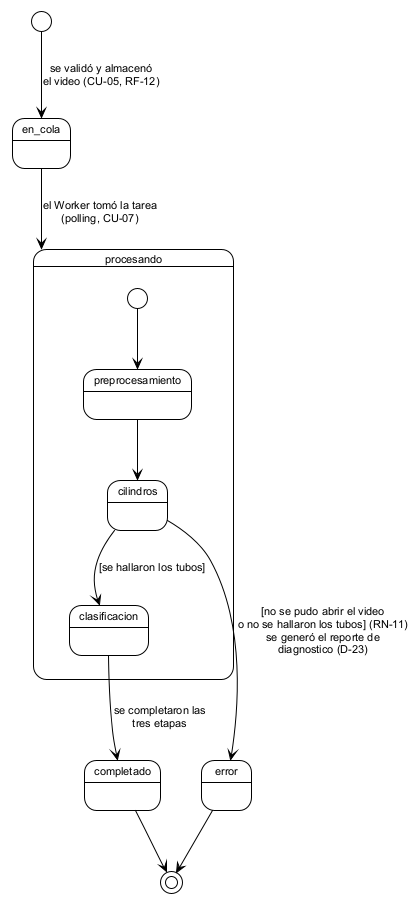
\includegraphics[width=0.85\textwidth]{figures/mermaid/estados_analisis}
\caption{Diagrama de estados de un análisis [autoría propia].}
\label{fig:estados_analisis}
\end{figure}

Un experimento agrupa varias tandas, cada una con su propio análisis, así que
el estado que ve el investigador en el dashboard (Figura~\ref{fig:estados_experimento})
es un valor calculado, no una columna de \texttt{EXPERIMENTO} (ver CU-21, RF-23):
se deriva del conjunto de análisis de todas sus tandas, con precedencia
error > procesando > en cola > completado cuando coexisten tandas en
distintos estados.

\begin{figure}[H]
\centering
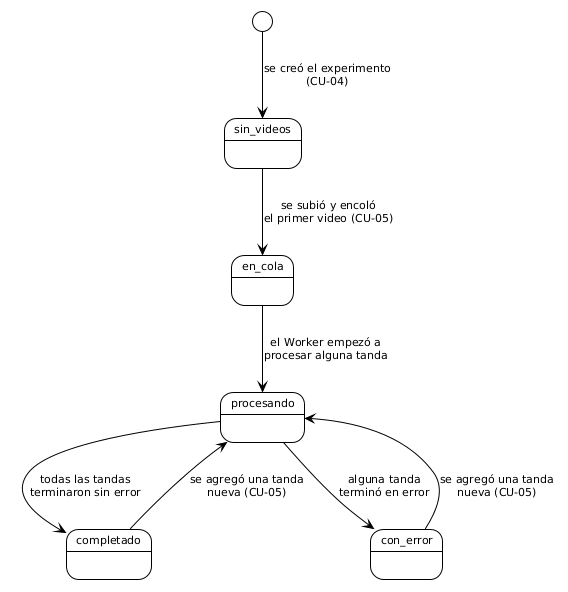
\includegraphics[width=0.85\textwidth]{figures/mermaid/estados_experimento}
\caption{Diagrama de estados agregado de un experimento [autoría propia].}
\label{fig:estados_experimento}
\end{figure}

\subsection{Separación por espécimen}

Los cilindros se graban en una sola toma lateral. La asignación de cada ROI a un
espécimen usa su posición horizontal en el encuadre: se ordena de izquierda a
derecha, produciendo una numeración consistente entre sesiones mientras el
encuadre no cambie. Si el número de
cilindros detectados es menor al esperado, el sistema reporta cuáles especímenes
pudo procesar y cuáles no, en lugar de abortar el análisis completo.

% -----------------------------------------------------------
\section{Diseño de la base de datos}
% -----------------------------------------------------------

El diseño de la base de datos parte de un modelo conceptual que identifica las
entidades del dominio y las relaciones entre ellas, sin entrar en detalles de
implementación. A partir de ese modelo se deriva el esquema físico que especifica
las tablas, columnas y tipos de datos concretos de PostgreSQL.

La Figura~\ref{fig:der} muestra el diagrama entidad-relación (DER) conceptual del
sistema. Las entidades principales son \textbf{USUARIO}, \textbf{EXPERIMENTO},
\textbf{GRUPO}, \textbf{TANDA}, \textbf{ESPECIMEN}, \textbf{VIDEO} y
\textbf{ANALISIS}. Las relaciones entre ellas definen el flujo central del
sistema: un usuario crea experimentos; cada experimento se organiza en grupos
(control, referencia, tratamiento); cada grupo se graba en una o más tandas de
hasta cuatro especímenes; cada tanda tiene uno o dos videos (Día~1 y/o Día~2); y
cada video se procesa mediante un análisis que produce observaciones de conducta
por espécimen (\textbf{OBSERVACION}, \textbf{SEGUNDO}, \textbf{INTERVALO},
\textbf{PRESENTA}, \textbf{CONDUCTA}). Un usuario puede además ser \textbf{ADMINISTRADOR}, modelado
como subtipo con permisos adicionales. Las entidades \textbf{REPORTE} y
\textbf{NOTIFICACION} se derivan también del experimento.

\begin{sidewaysfigure}
\centering
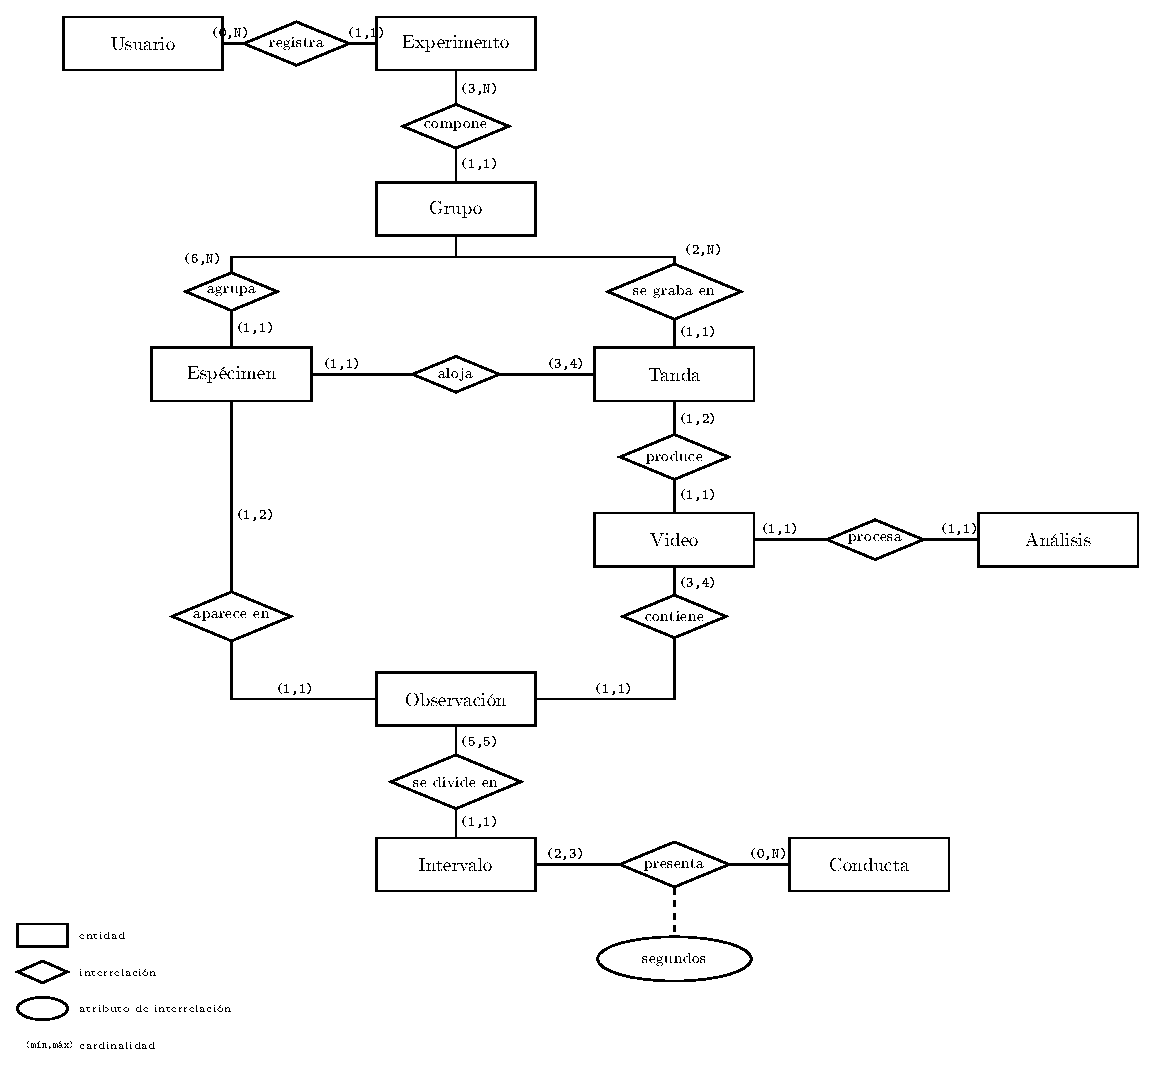
\includegraphics[width=\textheight, height=\textwidth, keepaspectratio]{diagramas/esquema_conceptual}
\caption{Diagrama entidad-relación conceptual del sistema [autoría propia].}
\label{fig:der}
\end{sidewaysfigure}

A partir del DER se derivó el esquema físico aplicando las reglas de conversión
al modelo relacional: cada entidad se convierte en una tabla, cada relación se
implementa mediante claves foráneas, y se agregan las columnas de control que
necesita el pipeline (\texttt{ANALISIS.estado}, \texttt{ANALISIS.etapa}) junto
con la marca de tiempo propia de cada tabla (\texttt{fechaCarga},
\texttt{fechaCreacion}, \texttt{fechaAnalisis}, \texttt{fechaGeneracion}). La
Figura~\ref{fig:er} muestra el resultado.

\begin{figure}[p]
\centering
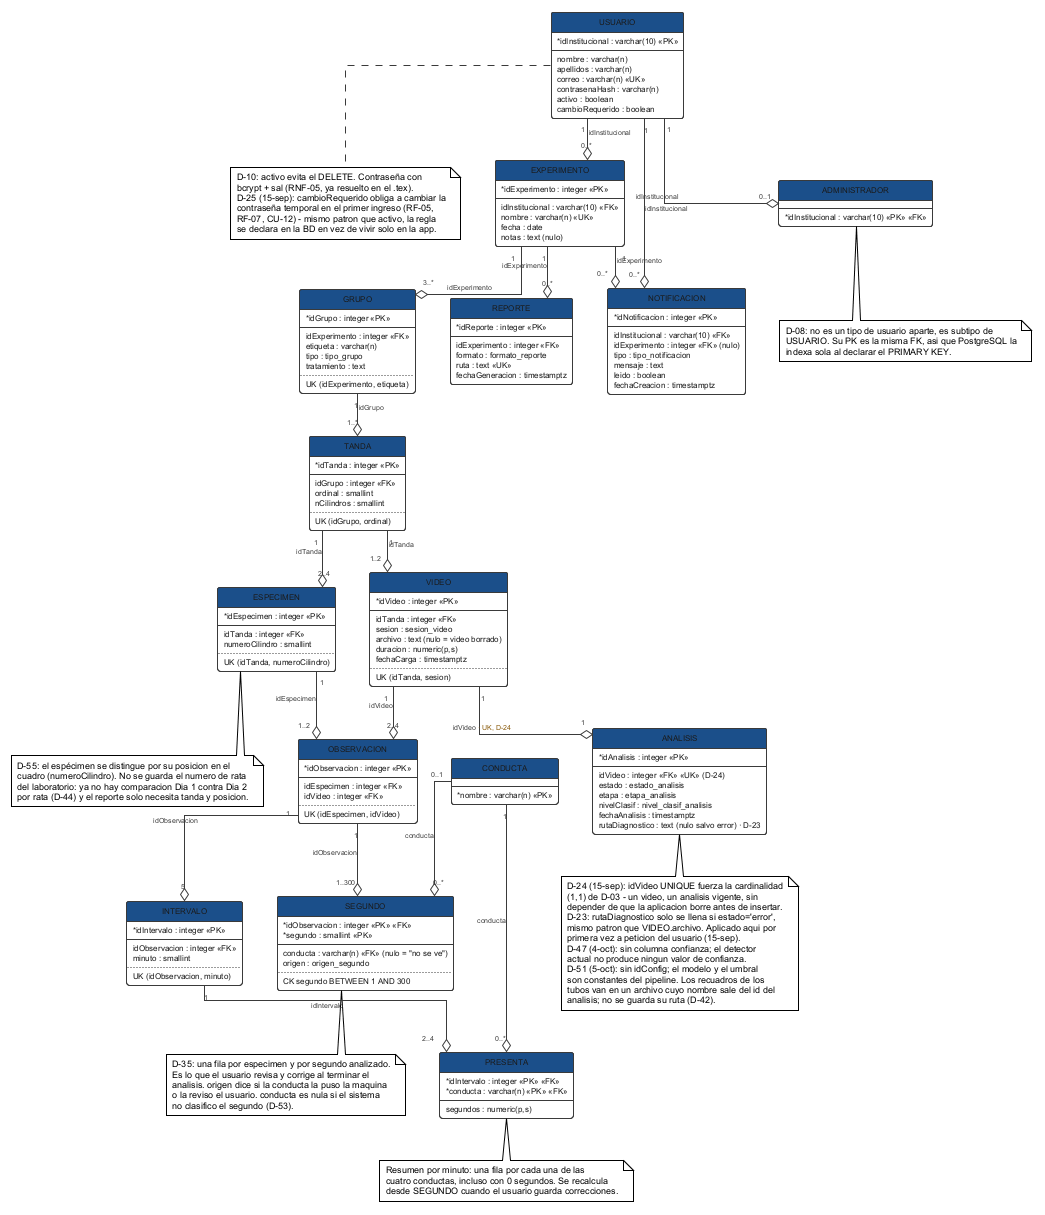
\includegraphics[width=\textwidth, height=0.90\textheight, keepaspectratio]{figures/mermaid/esquema_fisico}
\caption{Esquema físico de la base de datos [autoría propia].}
\label{fig:er}
\end{figure}

Las tablas están organizadas en cuatro grupos funcionales:

\textbf{Usuarios y acceso.}
\begin{itemize}
  \item \textbf{USUARIO}: credenciales (correo, hash de contraseña con
        bcrypt), nombre, apellidos, bandera \texttt{activo} (baja lógica,
        nunca se borra un usuario con experimentos) y bandera
        \texttt{cambioRequerido} que obliga a cambiar la contraseña temporal
        en el primer ingreso cuando la cuenta fue creada por el administrador
        (ver RF-05, RF-07).

  \item \textbf{ADMINISTRADOR}: subtipo de \texttt{USUARIO} (0,1). Un
        usuario aparece aquí solo si tiene permisos de administración; su
        ausencia significa que es investigador simple (ver D-08).
\end{itemize}

\textbf{Experimentos y material de video.}
\begin{itemize}
  \item \textbf{EXPERIMENTO}: nombre único, fecha y notas opcionales, con
        referencia al usuario propietario (ver RF-11). Todos los investigadores pueden
        consultar cualquier experimento del laboratorio (ver RN-08).

  \item \textbf{GRUPO}: cada grupo experimental (control, referencia o
        tratamiento) dentro de un experimento, con su etiqueta y su
        tratamiento o condición.

  \item \textbf{TANDA}: cada sesión de grabación de hasta cuatro especímenes
        dentro de un grupo, numerada por orden (A, B, C...).

  \item \textbf{ESPECIMEN}: un registro por espécimen dentro de su tanda,
        identificado por su número dentro del grupo y su posición de
        cilindro dentro de la tanda.

  \item \textbf{VIDEO}: uno o dos videos por tanda (Día~1 y/o Día~2), con
        ruta de almacenamiento, duración y fecha de carga. La ruta queda vacía
        cuando el archivo ya se borró (ver RF-25, RN-05); la fila se conserva
        porque los resultados la referencian.
\end{itemize}

\textbf{Análisis.}
\begin{itemize}
  \item \textbf{ANALISIS}: ejecución del pipeline sobre un video. Registra
        estado, etapa actual, nivel de clasificación (preciso o agrupado), la
        ruta al archivo con los recuadros de los tubos que usa la pantalla de
        revisión y, cuando falla, la ruta al reporte de diagnóstico (ver D-23).
\end{itemize}

El modelo del clasificador y el umbral de confianza (0.80) no se guardan en la
base de datos: ningún requisito permite cambiarlos, así que son constantes del
pipeline y se documentan en el Capítulo~6.

\textbf{Resultados, reportes y notificaciones.}
\begin{itemize}
  \item \textbf{OBSERVACION}: vincula un espécimen con el video en el que
        fue analizado.

  \item \textbf{INTERVALO}: cada minuto analizado dentro de una observación.

  \item \textbf{CONDUCTA}: catálogo cerrado de las cuatro conductas (nado
        activo, inmovilidad, escalamiento y conducta activa, esta última
        cuando el clasificador no decide entre nado y escalamiento; ver RN-13).

  \item \textbf{SEGUNDO}: una fila por espécimen y por segundo analizado, con
        la conducta asignada (o ninguna, si el espécimen no se ve), la
        propuesta original del sistema y el origen de la etiqueta (propuesta del
        sistema, confirmada, corregida o dudosa). Es lo que el usuario revisa y
        corrige al terminar el análisis (ver RF-32).

  \item \textbf{PRESENTA}: segundos de cada conducta dentro de cada
        intervalo. Es la fuente de los tiempos totales y del desglose
        por minuto, y se recalcula a partir de \texttt{SEGUNDO} cada vez que
        el usuario guarda correcciones.

  \item \textbf{REPORTE}: referencia a los archivos PDF, CSV y XLSX
        generados, con su ruta y fecha de creación. Se conservan aunque el
        video original haya sido eliminado (ver RN-06).

  \item \textbf{NOTIFICACION}: avisos al investigador sobre eventos del
        sistema, vinculados al usuario y, cuando aplica, al experimento
        correspondiente.
\end{itemize}

El diccionario de datos completo, con el tipo, las restricciones y la descripción
de cada columna, está en el Apéndice~\ref{ap:diccionario}.

% -----------------------------------------------------------
\section{Normalización de la base de datos}
\label{sec:normalizacion}
% -----------------------------------------------------------

La base de datos usa PostgreSQL como gestor relacional. Los datos del sistema
tienen una estructura jerárquica natural: un experimento se organiza en grupos,
cada grupo se graba en tandas de hasta cuatro especímenes, cada tanda tiene uno
o dos videos, y cada video se analiza produciendo resultados desglosados por
espécimen, por conducta y por minuto. Esa jerarquía se representa con integridad
referencial entre tablas relacionadas, sin repetir información en varios
lugares.

El proceso de normalización siguió las tres primeras formas normales definidas
por Codd \cite{codd1970} y descritas por Elmasri y Navathe \cite{elmasri2015}.
La motivación es práctica: si el nombre de un experimento se almacena en una sola
tabla, actualizarlo requiere una instrucción \texttt{UPDATE} en un solo lugar; si
estuviese copiado en las tablas de videos y de resultados, una actualización parcial
produciría registros con datos contradictorios. Normalizar también hace que el
esquema sea más fácil de mantener cuando el sistema evolucione durante TT-II.

Las quince relaciones del sistema son: \texttt{USUARIO}, \texttt{ADMINISTRADOR},
\texttt{EXPERIMENTO}, \texttt{GRUPO}, \texttt{TANDA}, \texttt{ESPECIMEN},
\texttt{VIDEO}, \texttt{ANALISIS},
\texttt{OBSERVACION}, \texttt{SEGUNDO}, \texttt{INTERVALO}, \texttt{CONDUCTA},
\texttt{PRESENTA}, \texttt{REPORTE} y \texttt{NOTIFICACION}. Las subsecciones siguientes explican
cómo se aplicó cada forma normal sobre este conjunto.

\subsection{Primera Forma Normal (1FN)}

La 1FN exige que cada columna almacene un único valor atómico ---sin listas,
conjuntos ni estructuras anidadas--- y que cada tabla tenga una clave primaria que
identifique cada fila de forma única \cite{codd1970}.

En el diseño inicial, las etiquetas de un espécimen podrían haberse guardado como
una lista dentro de \texttt{OBSERVACION}: un solo campo con las 300 conductas del
video, una por segundo. Eso viola la 1FN porque un campo único contendría cientos
de valores. Esas etiquetas se extrajeron a \texttt{SEGUNDO}, donde cada segundo
ocupa su propia fila con su conducta, su propuesta y su origen. Así
es posible consultar o corregir un segundo en la revisión sin reescribir la lista
completa ni parsear texto.

Los totales por minuto siguen el mismo principio, pero evitando además una
columna por conducta: en vez de columnas fijas para nado, inmovilidad y
escalamiento, cada combinación de intervalo y conducta es una fila en
\texttt{PRESENTA}, con su propia columna \texttt{segundos}. Esto evitó tener que
agregar una columna nueva cuando se incorporó una cuarta conducta (la conducta
activa), y permite consultar todas las conductas de un intervalo con una sola
condición sobre la clave foránea, en vez de una columna por caso. Todas las
tablas con clave subrogada usan un campo entero autogenerado como clave
primaria.

\subsection{Segunda Forma Normal (2FN)}

Una tabla en 2FN cumple la 1FN y, además, cada columna no clave depende de la clave
primaria \emph{completa} \cite{elmasri2015}. Esto es relevante cuando la clave
primaria es compuesta.

El caso compuesto del esquema es \texttt{PRESENTA}, cuya clave primaria es el par
(\texttt{idIntervalo}, \texttt{conducta}). Su única columna no clave,
\texttt{segundos}, depende de ambas partes de la clave a la vez: son los segundos
que esa conducta específica ocupó dentro de ese intervalo específico, no un dato
de la conducta en general ni del intervalo en general. Por eso no hay dependencia
parcial dentro de \texttt{PRESENTA} mismo. Pero si ahí también se hubiera
guardado una descripción de la conducta, esa columna dependería solo de
\texttt{conducta}, no del par completo. Esa es la razón por la que
\texttt{CONDUCTA} es un catálogo aparte: su nombre y cualquier atributo propio de
la conducta viven ahí, no repetidos en cada fila de \texttt{PRESENTA}.

\texttt{SEGUNDO} también tiene clave compuesta (\texttt{idObservacion},
\texttt{segundo}). Sus columnas no clave ---la conducta asignada, la propuesta
original y el origen de la etiqueta--- describen ese segundo específico de esa
observación específica, así que dependen de la clave completa y no de una de sus
partes.

\subsection{Tercera Forma Normal (3FN)}

Una tabla en 3FN cumple la 2FN y no tiene dependencias transitivas: ninguna columna
no clave depende de otra columna no clave \cite{elmasri2015}.

El caso principal está en la cadena \texttt{GRUPO}--\texttt{TANDA}--\texttt{ESPECIMEN}.
Un diseño con una fila por espécimen, como una hoja de cálculo, guardaría en
\texttt{ESPECIMEN} el tipo y el tratamiento de su grupo junto con su tanda. Eso
genera una dependencia transitiva: \texttt{tipo} y \texttt{tratamiento} dependen
de \texttt{idTanda} (a través del grupo de esa tanda), no de
\texttt{idEspecimen}, y \texttt{idTanda} no es clave candidata de
\texttt{ESPECIMEN}, porque en una tanda hay de dos a cuatro especímenes. Corregir
el tratamiento de un grupo obligaría a tocar cada uno de sus especímenes, y uno que
se quedara sin corregir dejaría al grupo con dos tratamientos a la vez.

La solución fue que cada dato viva en la tabla de la que depende:
\texttt{tipo} y \texttt{tratamiento} en \texttt{GRUPO}, el grupo en
\texttt{TANDA} (\texttt{idGrupo}) y la tanda en \texttt{ESPECIMEN}
(\texttt{idTanda}). El tratamiento de un espécimen se obtiene siguiendo las
llaves foráneas y se guarda en un solo lugar.

Un segundo caso es \texttt{USUARIO}. El correo identifica al usuario en la
práctica, pero la clave primaria es \texttt{idInstitucional} (boleta o número de
empleado). Los campos \texttt{nombre}, \texttt{apellidos}, \texttt{activo} y
\texttt{cambioRequerido} dependen directamente de \texttt{idInstitucional}, no
del correo. El correo se declara como clave alterna (\texttt{UNIQUE}), no como
primaria: si algún día cambiara, no haría falta actualizar las claves foráneas en
\texttt{EXPERIMENTO} y \texttt{NOTIFICACION}.

\subsection{Forma Normal de Boyce--Codd (FNBC)}

La FNBC es más estricta que la 3FN: exige que todo determinante (toda columna o
conjunto de columnas del que dependan funcionalmente otras columnas) sea una
clave candidata de la tabla, no solo que las columnas no clave dependan de la
clave completa \cite{elmasri2015}. Una tabla puede cumplir 3FN y aun así violar
FNBC cuando tiene más de una clave candidata y alguno de sus determinantes no
coincide con ninguna de ellas.

La misma separación que resolvió la dependencia transitiva de la 3FN también
asegura la FNBC: con el tratamiento dentro de \texttt{ESPECIMEN},
\texttt{idTanda} sería un determinante de esa tabla que no es clave candidata. Al
llevar el tipo y el tratamiento a \texttt{GRUPO}, a \texttt{ESPECIMEN} solo le
quedan determinantes que sí son claves candidatas: su clave primaria
\texttt{idEspecimen} y su clave alterna (\texttt{idTanda},
\texttt{numeroCilindro}).

El resto de las relaciones se revisó una por una: en cada una, los únicos
determinantes son su clave primaria y, cuando la tiene, su clave alterna. Por
ejemplo, \texttt{GRUPO} tiene como determinantes \texttt{idGrupo} (primaria) y la
combinación (\texttt{idExperimento}, \texttt{etiqueta}) (alterna). Con eso, las
quince relaciones del esquema lógico cumplen FNBC.

Hay una excepción deliberada en el esquema físico: la tabla \texttt{ESPECIMEN}
repite la columna \texttt{idGrupo}, que ya se obtiene a través de \texttt{TANDA}
(de \texttt{idTanda} se deduce \texttt{idGrupo}, y \texttt{idTanda} no es clave de
\texttt{ESPECIMEN}). Por eso, en el esquema físico, esa tabla deja de cumplir FNBC.
Se aceptó como redundancia controlada (D-04) por dos razones: permite declarar en la
propia base de datos que el número de espécimen es único dentro de su grupo, y evita
pasar por \texttt{TANDA} cada vez que un reporte compara grupos. La aplicación no
envía esa columna: la calcula un disparador a partir de la tanda, así que no puede
quedar desactualizada. El esquema lógico no incluye la columna y por eso conserva la
FNBC.

\subsection{Resumen de formas normales aplicadas}

La Tabla~\ref{tab:normalizacion} consolida los principios de normalización aplicados,
las tablas afectadas y la decisión de diseño concreta en cada caso.

\begin{table}[H]
\centering
\caption{Formas normales aplicadas en el diseño de la base de datos.}
\label{tab:normalizacion}
\small
\begin{tabular}{|p{1.5cm}|p{4.0cm}|p{3.1cm}|p{4.4cm}|}
\hline
\textbf{Forma normal} & \textbf{Regla aplicada} & \textbf{Tabla(s) afectada(s)} & \textbf{Observación} \\
\hline
1FN &
  Valores atómicos; sin campos JSON ni listas en el esquema &
  \texttt{SEGUNDO}, \texttt{PRESENTA} &
  Cada segundo de un espécimen y cada conducta por intervalo ocupa su propia
  fila \\
\hline
1FN &
  Clave primaria que identifica cada fila de forma única &
  Las 15 relaciones &
  Clave subrogada autogenerada, salvo \texttt{USUARIO}/\texttt{ADMINISTRADOR}
  (\texttt{idInstitucional}), \texttt{CONDUCTA} (\texttt{nombre}) y
  \texttt{SEGUNDO} (clave compuesta \texttt{idObservacion}, \texttt{segundo}) \\
\hline
2FN &
  Eliminación de dependencias parciales &
  \texttt{PRESENTA}, \texttt{SEGUNDO}, \texttt{CONDUCTA} &
  \texttt{segundos} depende del par completo (\texttt{idIntervalo},
  \texttt{conducta}); las columnas de \texttt{SEGUNDO} dependen de
  (\texttt{idObservacion}, \texttt{segundo}); atributos de la conducta viven en
  \texttt{CONDUCTA} \\
\hline
3FN &
  Eliminación de dependencias transitivas entre columnas no clave &
  \texttt{GRUPO}, \texttt{TANDA}, \texttt{ESPECIMEN} &
  \texttt{tipo} y \texttt{tratamiento} viven en \texttt{GRUPO};
  \texttt{ESPECIMEN} solo referencia su tanda \\
\hline
3FN &
  Clave sustituta en lugar de dato de negocio como clave primaria &
  \texttt{USUARIO} &
  \texttt{idInstitucional} como primaria; correo declarado como clave alterna
  (\texttt{UNIQUE}) \\
\hline
FNBC &
  Todo determinante es clave candidata &
  Las 15 relaciones &
  Verificado relación por relación; en el esquema físico, \texttt{ESPECIMEN}
  repite \texttt{idGrupo} a propósito (D-04) \\
\hline
\end{tabular}
\end{table}

% -----------------------------------------------------------
\section{Diseño de la API REST}
% -----------------------------------------------------------

La API REST sigue las convenciones HTTP estándar \cite{grinberg2018}. Todos los
endpoints requieren autenticación con JWT salvo los de inicio de sesión y recuperación
de contraseña. Las respuestas usan JSON con una estructura consistente: campo
\texttt{data} para el resultado, \texttt{error} para mensajes de error y
\texttt{status} para el código HTTP.

La Tabla~\ref{tab:api} describe los endpoints principales agrupados por recurso.

\begin{longtable}{|p{1.4cm}|p{5.8cm}|p{4.8cm}|p{1.6cm}|}
\caption{Endpoints principales de la API REST.
\label{tab:api}}\\
\hline
\textbf{Método} & \textbf{Ruta} & \textbf{Descripción} & \textbf{Acceso} \\
\hline
\endfirsthead
\hline
\textbf{Método} & \textbf{Ruta} & \textbf{Descripción} & \textbf{Acceso} \\
\hline
\endhead
\hline
\endfoot

% --- Autenticación ---
POST   & \path{/auth/login}    & Inicia sesión; devuelve token JWT. & Público \\
\hline
POST   & \path{/auth/logout}   & Cierra la sesión; el navegador descarta el token. & Autenti\-cado \\
\hline
POST   & \path{/auth/recover}  & Envía enlace de recuperación por correo. & Público \\
\hline
PATCH  & \path{/auth/password} & Cambia la contraseña del usuario autenticado. & Autenti\-cado \\
\hline

% --- Experimentos ---
GET    & \path{/experiments}         & Lista todos los experimentos del laboratorio (ver RN-08). & Investiga\-dor \\
\hline
POST   & \path{/experiments}         & Crea un experimento con sus metadatos. & Investiga\-dor \\
\hline
GET    & \path{/experiments/{id}}    & Devuelve detalle y estado de un experimento. & Investiga\-dor \\
\hline

% --- Videos y análisis ---
POST   & \path{/experiments/{id}/groups/{grupo}/videos}  & Sube un video (Día~1 o Día~2) a una tanda del grupo indicado (se crea la tanda si no existe) y encola el análisis. & Investiga\-dor \\
\hline
GET    & \path{/experiments/{id}/status}  & Devuelve el progreso del análisis en porcentaje. & Investiga\-dor \\
\hline

% --- Resultados ---
GET    & \path{/experiments/{id}/results}          & Devuelve los resultados por espécimen y conducta. & Investiga\-dor \\
\hline
GET    & \path{/experiments/{id}/results/byminute} & Devuelve el desglose temporal por minuto. & Investiga\-dor \\
\hline
GET    & \path{/experiments/{id}/groups/{grupo}/tandas/{tanda}/comparison} & Devuelve la comparación Día~1 vs.\ Día~2 de esa tanda. & Investiga\-dor \\
\hline

% --- Reportes ---
GET    & \path{/experiments/{id}/report/pdf}  & Descarga el reporte en PDF. & Investiga\-dor \\
\hline
GET    & \path{/experiments/{id}/report/csv}  & Descarga los datos en CSV. & Investiga\-dor \\
\hline
GET    & \path{/experiments/{id}/report/xlsx} & Descarga los datos en XLSX. & Investiga\-dor \\
\hline

% --- Revisión segundo a segundo ---
GET    & \path{/experiments/{id}/analyses/{idAnalisis}/review}   & Devuelve los especímenes, las etiquetas de cada segundo y los recuadros de los tubos de un análisis completado. & Investiga\-dor \\
\hline
GET    & \path{/experiments/{id}/analyses/{idAnalisis}/video}    & Entrega el video de la revisión por partes, para poder adelantar y retroceder. & Investiga\-dor \\
\hline
PUT    & \path{/experiments/{id}/analyses/{idAnalisis}/segundos} & Guarda las correcciones por segundo y recalcula los totales por minuto. & Investiga\-dor \\
\hline

% --- Administración ---
GET    & \path{/admin/users}        & Lista todos los usuarios (filtrable por administrador/investigador y estado). & Admin \\
\hline
POST   & \path{/admin/users}        & Crea una cuenta de usuario con contraseña temporal. & Admin \\
\hline
PATCH  & \path{/admin/users/{id}}   & Modifica datos o desactiva una cuenta. & Admin \\
\hline
GET    & \path{/admin/system}       & Devuelve métricas del sistema: disco y cola. & Admin \\
\hline

\end{longtable}

% -----------------------------------------------------------
\section{Diseño de casos de uso}
% -----------------------------------------------------------

Los diagramas de casos de uso se construyen conforme a la especificación UML~2.5.1
\cite{omg_uml,iso19501}, usando actores, casos de uso y relaciones de
\textit{include} y \textit{extend} para representar el comportamiento observable
del sistema desde la perspectiva del usuario.

El sistema tiene dos actores principales: \textbf{Investigador} y
\textbf{Administrador}. El Investigador gestiona experimentos y consulta
resultados de cualquier investigador del laboratorio (ver RN-08); el Administrador
gestiona usuarios y monitorea el estado del sistema. El Administrador hereda todas
las capacidades del Investigador y además puede modificar y desactivar cuentas.

Los casos de uso están organizados en cinco paquetes funcionales. La
Figura~\ref{fig:cu_vision_general} muestra la visión general con los dos actores y
sus relaciones de alto nivel; las figuras siguientes detallan cada paquete.

\begin{figure}[H]
\centering
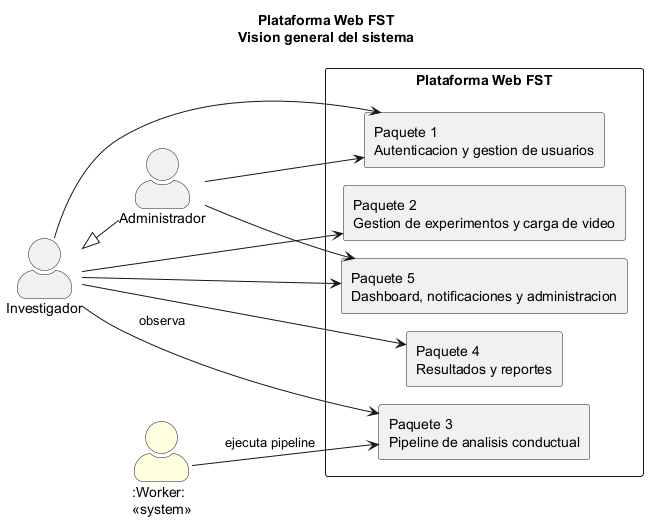
\includegraphics[width=\textwidth]{figures/mermaid/cu_vision_general}
\caption{Diagrama de casos de uso — visión general del sistema [autoría propia].}
\label{fig:cu_vision_general}
\end{figure}

\subsection{Paquete 1: Autenticación y gestión de usuarios}

Agrupa los flujos de acceso al sistema: inicio de sesión con correo y contraseña,
cierre de sesión y recuperación o cambio de contraseña. El flujo es idéntico para
Investigador y Administrador; la diferencia de permisos se resuelve dentro del
sistema una vez autenticados. Incluye además la gestión de cuentas a cargo del
Administrador (crear y desactivar), el cambio obligatorio de contraseña en el primer
acceso y la actualización del perfil propio.

\begin{figure}[H]
\centering
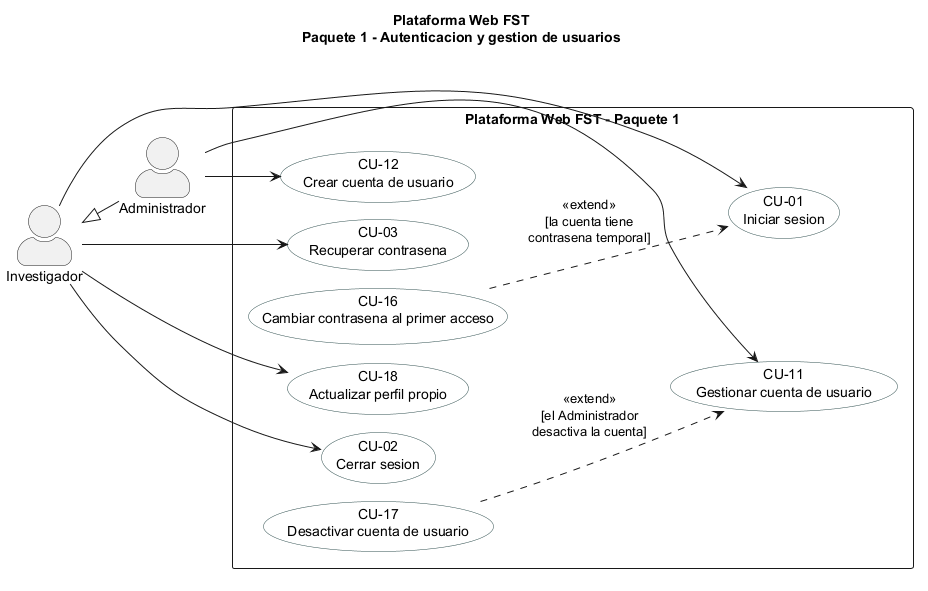
\includegraphics[width=\textwidth]{figures/mermaid/cu_paquete1}
\caption{Casos de uso — Paquete 1: Autenticación y gestión de usuarios [autoría propia].}
\label{fig:cu_paquete1}
\end{figure}

\subsection{Paquete 2: Gestión de experimentos y carga de video}

Cubre el ciclo de vida de un experimento: registrar sus datos (nombre, fecha y notas),
subir uno o dos videos por tanda en formato MP4 o MOV (al subir el primer video de cada
grupo se capturan su tipo, su tratamiento y el número de especímenes de la tanda) y
consultar el historial de experimentos del laboratorio (ver RN-08).

\begin{figure}[H]
\centering
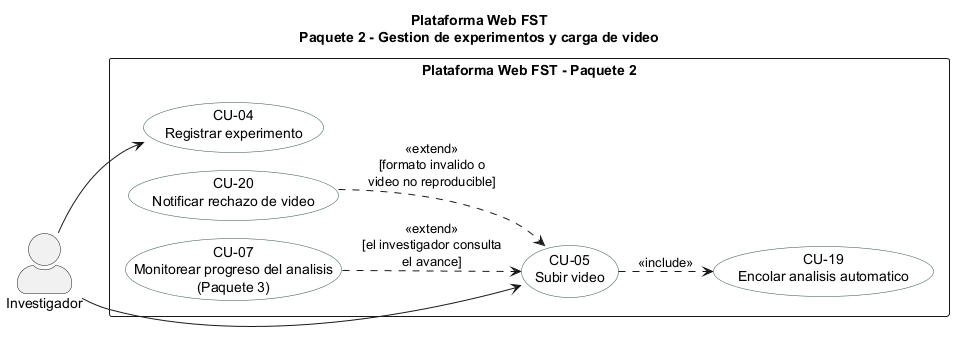
\includegraphics[width=\textwidth]{figures/mermaid/cu_paquete2}
\caption{Casos de uso — Paquete 2: Gestión de experimentos y carga de video [autoría propia].}
\label{fig:cu_paquete2}
\end{figure}

\subsection{Paquete 3: Análisis conductual}

Describe la interacción del investigador con el pipeline: monitorear el avance
del análisis por etapas y descargar el reporte de diagnóstico cuando el análisis termina
en error (ver RN-11). El pipeline lo ejecuta el \textit{Worker} de forma autónoma;
el investigador solo observa.

\begin{figure}[H]
\centering
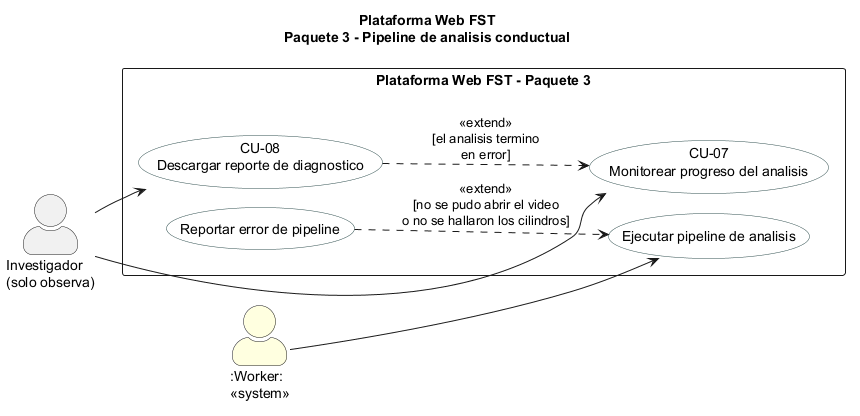
\includegraphics[width=\textwidth]{figures/mermaid/cu_paquete3}
\caption{Casos de uso — Paquete 3: Análisis conductual [autoría propia].}
\label{fig:cu_paquete3}
\end{figure}

\subsection{Paquete 4: Resultados y reportes}

Cubre la consulta de resultados una vez finalizado el análisis: tiempos por
espécimen y conducta, desglose por minuto, comparación entre los grupos del experimento con el Día~2,
descarga de reportes en PDF, CSV y XLSX y, cuando el análisis termina, revisión y corrección de las etiquetas segundo a segundo (ver
RF-32 y RN-14).

\begin{figure}[H]
\centering
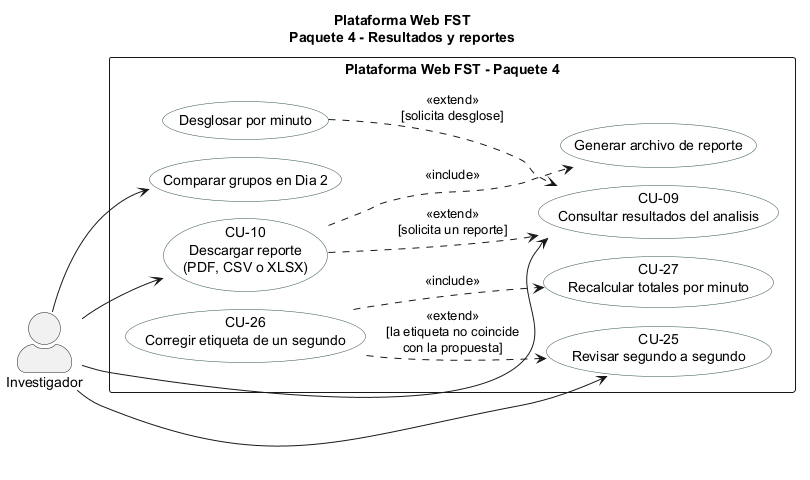
\includegraphics[width=\textwidth]{figures/mermaid/cu_paquete4}
\caption{Casos de uso — Paquete 4: Resultados y reportes [autoría propia].}
\label{fig:cu_paquete4}
\end{figure}

\subsection{Paquete 5: Dashboard, notificaciones y administración}

Reúne lo que el investigador ve al entrar (el \textit{dashboard} con la lista de
experimentos, sus filtros y los avisos de expiración de video), la eliminación de
experimentos, el borrado automático de videos y, para el Administrador, el listado de
usuarios, el monitoreo del estado del sistema (uso de disco, cola de análisis y alertas
de capacidad) y la gestión de los experimentos de todo el laboratorio.

\begin{figure}[H]
\centering
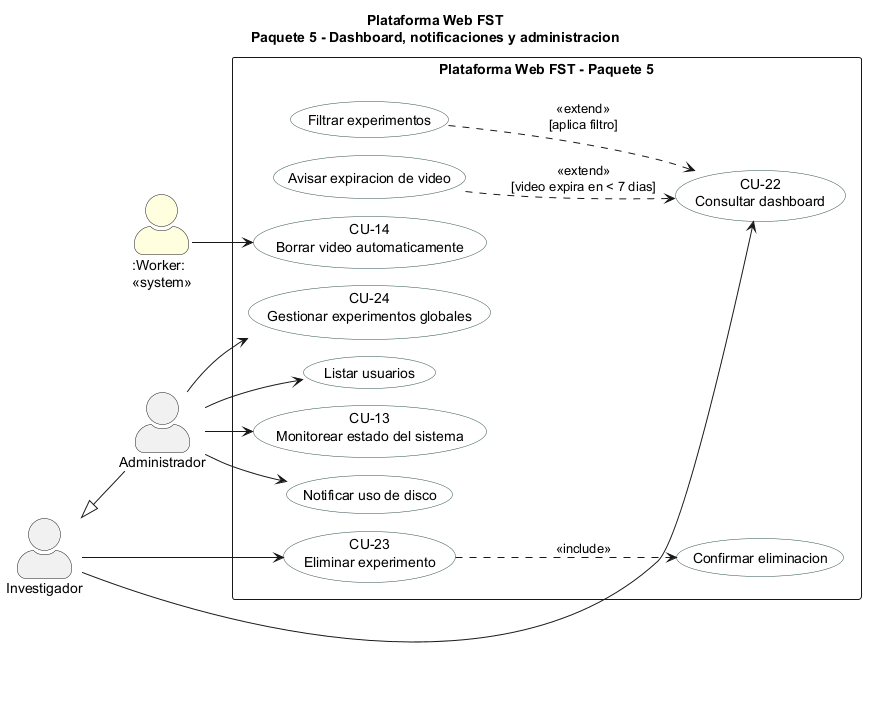
\includegraphics[width=\textwidth]{figures/mermaid/cu_paquete5}
\caption{Casos de uso — Paquete 5: Dashboard, notificaciones y administración [autoría propia].}
\label{fig:cu_paquete5}
\end{figure}

% -----------------------------------------------------------
\subsection{Especificación de casos de uso}
\label{sec:especificacion_cu}
% -----------------------------------------------------------

Para cada caso de uso identificado en los diagramas anteriores se presenta una ficha
completa que describe la interacción del actor con el sistema, los datos de entrada,
la información que el sistema devuelve y los eventos inesperados que pueden ocurrir.
Los casos de uso con identificador CU-xx son los mismos de las fichas; los que no lo
tienen en los diagramas son pasos o condiciones que cada ficha describe dentro de su
curso normal o alterno. La ficha CU-15 describe una regla de control de acceso que el
sistema aplica antes de las acciones de administración, por lo que no se dibuja como
caso de uso.

\renewcommand{\arraystretch}{1.35}

\subsubsection*{Paquete 1: Autenticación y gestión de usuarios}

\noindent\textbf{Iniciar sesión}

\noindent\small
\begin{tabular}{|p{2.8cm}|p{7.9cm}|p{4.0cm}|}
\hline
\textbf{Caso de Uso} & Iniciar sesión & \textbf{Identificador:} CU-01 \\
\hline
\textbf{Actores} & \multicolumn{2}{>{\raggedright\arraybackslash}p{12.4cm}|}{Investigador / Administrador} \\
\hline
\textbf{Tipo} & \multicolumn{2}{>{\raggedright\arraybackslash}p{12.4cm}|}{Primario} \\
\hline
\textbf{Referencias} & \multicolumn{2}{>{\raggedright\arraybackslash}p{12.4cm}|}{RF-01, RF-04. Extendido por: CU-16 (Cambiar contraseña al primer acceso).} \\
\hline
\textbf{Precondición} & \multicolumn{2}{>{\raggedright\arraybackslash}p{12.4cm}|}{El usuario tiene una cuenta creada por el Administrador.} \\
\hline
\textbf{Postcondición} & \multicolumn{2}{>{\raggedright\arraybackslash}p{12.4cm}|}{Sesión iniciada; JWT emitido y almacenado en el cliente; usuario redirigido al \textit{dashboard}.} \\
\hline
\textbf{Descripción} & \multicolumn{2}{>{\raggedright\arraybackslash}p{12.4cm}|}{Permite al usuario autenticarse en el sistema mediante correo electrónico y contraseña.} \\
\hline
\textbf{Resumen} & \multicolumn{2}{>{\raggedright\arraybackslash}p{12.4cm}|}{El usuario introduce sus credenciales; el sistema las valida, emite un JWT y redirige al \textit{dashboard}. Si las credenciales son incorrectas, se muestra un mensaje de error sin revelar cuál campo falló.} \\
\hline
\end{tabular}

\noindent
\begin{tabular}{|p{1.0cm}|p{3.7cm}|p{10.0cm}|}
\hline
\multicolumn{3}{|l|}{\textbf{Curso Normal}} \\
\hline
\textbf{Nro.} & \textbf{Ejecutor} & \textbf{Paso o Actividad} \\
\hline
1 & Inv. / Admin. & Abre la aplicación en el navegador web. \\
\hline
2 & Sistema & Muestra la pantalla de inicio de sesión con campos de correo y contraseña. \\
\hline
3 & Inv. / Admin. & Introduce su correo electrónico y contraseña. \\
\hline
4 & Sistema & Valida las credenciales contra la base de datos. \\
\hline
5 & Sistema & Emite un JWT y lo almacena en el cliente. \\
\hline
6 & Sistema & Redirige al usuario al \textit{dashboard} principal. \\
\hline
\end{tabular}

\noindent
\begin{tabular}{|p{1.0cm}|p{14.1cm}|}
\hline
\multicolumn{2}{|l|}{\textbf{Cursos Alternos}} \\
\hline
\textbf{Nro.} & \textbf{Descripción de acciones alternas} \\
\hline
4 & Credenciales incorrectas: el sistema muestra mensaje de error sin indicar cuál campo falló (ver RN-01). \\
\hline
\end{tabular}

\normalsize\bigskip

\noindent\rule{\linewidth}{0.4pt}

\noindent\textbf{Cerrar sesión}

\noindent\small
\begin{tabular}{|p{2.8cm}|p{7.9cm}|p{4.0cm}|}
\hline
\textbf{Caso de Uso} & Cerrar sesión & \textbf{Identificador:} CU-02 \\
\hline
\textbf{Actores} & \multicolumn{2}{>{\raggedright\arraybackslash}p{12.4cm}|}{Investigador / Administrador} \\
\hline
\textbf{Tipo} & \multicolumn{2}{>{\raggedright\arraybackslash}p{12.4cm}|}{Primario} \\
\hline
\textbf{Referencias} & \multicolumn{2}{>{\raggedright\arraybackslash}p{12.4cm}|}{RF-02} \\
\hline
\textbf{Precondición} & \multicolumn{2}{>{\raggedright\arraybackslash}p{12.4cm}|}{Sesión activa con JWT válido.} \\
\hline
\textbf{Postcondición} & \multicolumn{2}{>{\raggedright\arraybackslash}p{12.4cm}|}{Token JWT descartado en el navegador; usuario redirigido a la pantalla de inicio de sesión.} \\
\hline
\textbf{Descripción} & \multicolumn{2}{>{\raggedright\arraybackslash}p{12.4cm}|}{Permite al usuario terminar su sesión descartando el token de autenticación activo.} \\
\hline
\textbf{Resumen} & \multicolumn{2}{>{\raggedright\arraybackslash}p{12.4cm}|}{El usuario selecciona la opción de cierre de sesión; el navegador descarta el JWT y redirige a la pantalla de inicio de sesión; el servidor no guarda tokens cancelados.} \\
\hline
\end{tabular}

\noindent
\begin{tabular}{|p{1.0cm}|p{3.7cm}|p{10.0cm}|}
\hline
\multicolumn{3}{|l|}{\textbf{Curso Normal}} \\
\hline
\textbf{Nro.} & \textbf{Ejecutor} & \textbf{Paso o Actividad} \\
\hline
1 & Inv. / Admin. & Selecciona «Cerrar sesión» en el menú de usuario, disponible desde cualquier pantalla. \\
\hline
2 & Sistema & Descarta el JWT activo en el navegador (el servidor no guarda tokens cancelados). \\
\hline
3 & Sistema & Redirige al usuario a la pantalla de inicio de sesión. \\
\hline
\end{tabular}

\noindent
\begin{tabular}{|p{1.0cm}|p{14.1cm}|}
\hline
\multicolumn{2}{|l|}{\textbf{Cursos Alternos}} \\
\hline
\textbf{Nro.} & \textbf{Descripción de acciones alternas} \\
\hline
--- & No se identifican cursos alternos para este caso de uso. \\
\hline
\end{tabular}

\normalsize\bigskip

\noindent\rule{\linewidth}{0.4pt}

\noindent\textbf{Recuperar contraseña}

\noindent\small
\begin{tabular}{|p{2.8cm}|p{7.9cm}|p{4.0cm}|}
\hline
\textbf{Caso de Uso} & Recuperar contraseña & \textbf{Identificador:} CU-03 \\
\hline
\textbf{Actores} & \multicolumn{2}{>{\raggedright\arraybackslash}p{12.4cm}|}{Investigador / Administrador} \\
\hline
\textbf{Tipo} & \multicolumn{2}{>{\raggedright\arraybackslash}p{12.4cm}|}{Secundario} \\
\hline
\textbf{Referencias} & \multicolumn{2}{>{\raggedright\arraybackslash}p{12.4cm}|}{RF-03} \\
\hline
\textbf{Precondición} & \multicolumn{2}{>{\raggedright\arraybackslash}p{12.4cm}|}{El usuario tiene una cuenta activa con correo electrónico registrado.} \\
\hline
\textbf{Postcondición} & \multicolumn{2}{>{\raggedright\arraybackslash}p{12.4cm}|}{Enlace de restablecimiento enviado al correo; nueva contraseña establecida y sesión disponible.} \\
\hline
\textbf{Descripción} & \multicolumn{2}{>{\raggedright\arraybackslash}p{12.4cm}|}{Permite al usuario restablecer su contraseña mediante un enlace temporal enviado a su correo registrado.} \\
\hline
\textbf{Resumen} & \multicolumn{2}{>{\raggedright\arraybackslash}p{12.4cm}|}{El usuario solicita el restablecimiento; el sistema envía un enlace de validez limitada al correo del usuario; el usuario accede al enlace y establece una nueva contraseña.} \\
\hline
\end{tabular}

\noindent
\begin{tabular}{|p{1.0cm}|p{3.7cm}|p{10.0cm}|}
\hline
\multicolumn{3}{|l|}{\textbf{Curso Normal}} \\
\hline
\textbf{Nro.} & \textbf{Ejecutor} & \textbf{Paso o Actividad} \\
\hline
1 & Inv. / Admin. & Selecciona «Olvidé mi contraseña» en la pantalla de inicio de sesión. \\
\hline
2 & Sistema & Solicita el correo electrónico registrado. \\
\hline
3 & Inv. / Admin. & Introduce su correo electrónico. \\
\hline
4 & Sistema & Envía un enlace de restablecimiento con validez de tiempo limitado al correo indicado. \\
\hline
5 & Inv. / Admin. & Accede al enlace recibido e introduce una nueva contraseña. \\
\hline
6 & Sistema & Actualiza la contraseña en la base de datos y redirige al inicio de sesión. \\
\hline
\end{tabular}

\noindent
\begin{tabular}{|p{1.0cm}|p{14.1cm}|}
\hline
\multicolumn{2}{|l|}{\textbf{Cursos Alternos}} \\
\hline
\textbf{Nro.} & \textbf{Descripción de acciones alternas} \\
\hline
3 & El correo no está registrado: el sistema responde con el mismo mensaje que si existiera, para no exponer información sobre cuentas registradas. \\
\hline
5 & El enlace ya expiró: el sistema informa que el enlace no es válido y solicita reiniciar el proceso desde el paso 1. \\
\hline
\end{tabular}

\normalsize\bigskip

\noindent\rule{\linewidth}{0.4pt}

\noindent\textbf{Verificar pertenencia a Administrador}

\noindent\small
\begin{tabular}{|p{2.8cm}|p{7.9cm}|p{4.0cm}|}
\hline
\textbf{Caso de Uso} & Verificar pertenencia a Administrador & \textbf{Identificador:} CU-15 \\
\hline
\textbf{Actores} & \multicolumn{2}{>{\raggedright\arraybackslash}p{12.4cm}|}{Sistema} \\
\hline
\textbf{Tipo} & \multicolumn{2}{>{\raggedright\arraybackslash}p{12.4cm}|}{Regla de control de acceso (se aplica antes de CU-11, CU-12, CU-13 y CU-17)} \\
\hline
\textbf{Referencias} & \multicolumn{2}{>{\raggedright\arraybackslash}p{12.4cm}|}{RF-04} \\
\hline
\textbf{Precondición} & \multicolumn{2}{>{\raggedright\arraybackslash}p{12.4cm}|}{Sesión activa (JWT válido).} \\
\hline
\textbf{Postcondición} & \multicolumn{2}{>{\raggedright\arraybackslash}p{12.4cm}|}{Se confirma o rechaza que el usuario pertenece a \texttt{ADMINISTRADOR}; la acción de administración solicitada continúa o se rechaza con error 403.} \\
\hline
\textbf{Descripción} & \multicolumn{2}{>{\raggedright\arraybackslash}p{12.4cm}|}{Antes de ejecutar cualquier acción de administración (crear cuenta, desactivar cuenta, listar usuarios o monitorear el sistema), el sistema verifica si el usuario autenticado pertenece a la tabla \texttt{ADMINISTRADOR}, sin importar si la interfaz ya ocultó la opción.} \\
\hline
\textbf{Resumen} & \multicolumn{2}{>{\raggedright\arraybackslash}p{12.4cm}|}{Al invocar cualquiera de las cuatro acciones de administración, el sistema consulta si el \texttt{idInstitucional} del usuario autenticado tiene una fila en \texttt{ADMINISTRADOR}. Si no la tiene, rechaza la solicitud con error 403, incluso si la petición no pasó por la interfaz (por ejemplo, una llamada directa a la API).} \\
\hline
\end{tabular}

\noindent
\begin{tabular}{|p{1.0cm}|p{3.7cm}|p{10.0cm}|}
\hline
\multicolumn{3}{|l|}{\textbf{Curso Normal}} \\
\hline
\textbf{Nro.} & \textbf{Ejecutor} & \textbf{Paso o Actividad} \\
\hline
1 & Sistema & Recibe la solicitud de una acción de administración (crear/desactivar cuenta, listar usuarios o monitorear el sistema). \\
\hline
2 & Sistema & Consulta si el \texttt{idInstitucional} del usuario autenticado tiene registro en \texttt{ADMINISTRADOR}. \\
\hline
3 & Sistema & Si existe el registro, permite continuar con la acción solicitada. \\
\hline
\end{tabular}

\noindent
\begin{tabular}{|p{1.0cm}|p{14.1cm}|}
\hline
\multicolumn{2}{|l|}{\textbf{Cursos Alternos}} \\
\hline
\textbf{Nro.} & \textbf{Descripción de acciones alternas} \\
\hline
2 & El usuario no tiene registro en \texttt{ADMINISTRADOR}: el sistema rechaza la solicitud con error 403 (no autorizado), sin importar si la petición vino de la interfaz o de una llamada directa a la API. \\
\hline
\end{tabular}

\normalsize\bigskip

\noindent\rule{\linewidth}{0.4pt}

\noindent\textbf{Cambiar contraseña al primer acceso}

\noindent\small
\begin{tabular}{|p{2.8cm}|p{7.9cm}|p{4.0cm}|}
\hline
\textbf{Caso de Uso} & Cambiar contraseña al primer acceso & \textbf{Identificador:} CU-16 \\
\hline
\textbf{Actores} & \multicolumn{2}{>{\raggedright\arraybackslash}p{12.4cm}|}{Investigador / Administrador} \\
\hline
\textbf{Tipo} & \multicolumn{2}{>{\raggedright\arraybackslash}p{12.4cm}|}{Secundario (\textit{<<extend>>} de CU-01 Iniciar sesión, condición: la cuenta tiene contraseña temporal)} \\
\hline
\textbf{Referencias} & \multicolumn{2}{>{\raggedright\arraybackslash}p{12.4cm}|}{RF-05. Extiende: CU-01 (Iniciar sesión).} \\
\hline
\textbf{Precondición} & \multicolumn{2}{>{\raggedright\arraybackslash}p{12.4cm}|}{Usuario autenticado con contraseña temporal asignada por el Administrador; primer ingreso al sistema.} \\
\hline
\textbf{Postcondición} & \multicolumn{2}{>{\raggedright\arraybackslash}p{12.4cm}|}{Contraseña actualizada en la base de datos; marca de «cambio obligatorio» eliminada; acceso completo habilitado.} \\
\hline
\textbf{Descripción} & \multicolumn{2}{>{\raggedright\arraybackslash}p{12.4cm}|}{El sistema obliga al usuario a establecer una contraseña propia antes de permitir el acceso a cualquier funcionalidad del sistema.} \\
\hline
\textbf{Resumen} & \multicolumn{2}{>{\raggedright\arraybackslash}p{12.4cm}|}{Al detectar la marca de «cambio obligatorio», el sistema redirige al usuario a la pantalla de cambio de contraseña. El usuario introduce la nueva contraseña; el sistema la valida, la actualiza y habilita el acceso completo.} \\
\hline
\end{tabular}

\noindent
\begin{tabular}{|p{1.0cm}|p{3.7cm}|p{10.0cm}|}
\hline
\multicolumn{3}{|l|}{\textbf{Curso Normal}} \\
\hline
\textbf{Nro.} & \textbf{Ejecutor} & \textbf{Paso o Actividad} \\
\hline
1 & Sistema & Detecta la marca de «cambio obligatorio» en la cuenta tras la autenticación inicial. \\
\hline
2 & Sistema & Redirige al usuario a la pantalla de cambio de contraseña antes de acceder al \textit{dashboard}. \\
\hline
3 & Inv. / Admin. & Introduce la nueva contraseña y la confirma. \\
\hline
4 & Sistema & Valida que la nueva contraseña cumple los requisitos de seguridad y que no coincide con la contraseña temporal. \\
\hline
5 & Sistema & Actualiza la contraseña, elimina la marca de «cambio obligatorio» y redirige al \textit{dashboard}. \\
\hline
\end{tabular}

\noindent
\begin{tabular}{|p{1.0cm}|p{14.1cm}|}
\hline
\multicolumn{2}{|l|}{\textbf{Cursos Alternos}} \\
\hline
\textbf{Nro.} & \textbf{Descripción de acciones alternas} \\
\hline
4 & La nueva contraseña no cumple los requisitos mínimos: el sistema muestra los criterios incumplidos y solicita que el usuario introduzca una contraseña diferente. \\
\hline
\end{tabular}

\normalsize\bigskip

\noindent\rule{\linewidth}{0.4pt}

\noindent\textbf{Desactivar cuenta de usuario}

\noindent\small
\begin{tabular}{|p{2.8cm}|p{7.9cm}|p{4.0cm}|}
\hline
\textbf{Caso de Uso} & Desactivar cuenta de usuario & \textbf{Identificador:} CU-17 \\
\hline
\textbf{Actores} & \multicolumn{2}{>{\raggedright\arraybackslash}p{12.4cm}|}{Administrador} \\
\hline
\textbf{Tipo} & \multicolumn{2}{>{\raggedright\arraybackslash}p{12.4cm}|}{Secundario (\textit{<<extend>>} de CU-11 Gestionar cuenta de usuario, condición: el Administrador desactiva la cuenta)} \\
\hline
\textbf{Referencias} & \multicolumn{2}{>{\raggedright\arraybackslash}p{12.4cm}|}{RF-05. Extiende: CU-11 (Gestionar cuenta de usuario).} \\
\hline
\textbf{Precondición} & \multicolumn{2}{>{\raggedright\arraybackslash}p{12.4cm}|}{Sesión activa; el usuario pertenece a \texttt{ADMINISTRADOR} (ver CU-15); cuenta objetivo en estado activo.} \\
\hline
\textbf{Postcondición} & \multicolumn{2}{>{\raggedright\arraybackslash}p{12.4cm}|}{Cuenta marcada como inactiva; el usuario no puede iniciar sesión hasta que el Administrador reactive la cuenta.} \\
\hline
\textbf{Descripción} & \multicolumn{2}{>{\raggedright\arraybackslash}p{12.4cm}|}{Permite al Administrador inhabilitar el acceso de un investigador sin eliminar su cuenta ni sus datos asociados.} \\
\hline
\textbf{Resumen} & \multicolumn{2}{>{\raggedright\arraybackslash}p{12.4cm}|}{El Administrador selecciona la cuenta a desactivar y confirma la acción. El sistema marca la cuenta como inactiva; el usuario queda impedido de iniciar sesión.} \\
\hline
\end{tabular}

\noindent
\begin{tabular}{|p{1.0cm}|p{3.7cm}|p{10.0cm}|}
\hline
\multicolumn{3}{|l|}{\textbf{Curso Normal}} \\
\hline
\textbf{Nro.} & \textbf{Ejecutor} & \textbf{Paso o Actividad} \\
\hline
1 & Administrador & Selecciona la cuenta objetivo en la lista de usuarios y elige «Desactivar cuenta». \\
\hline
2 & Sistema & Solicita confirmación de la acción. \\
\hline
3 & Administrador & Confirma la desactivación. \\
\hline
4 & Sistema & Marca la cuenta como inactiva en la base de datos. \\
\hline
5 & Sistema & Muestra confirmación de la operación en el panel de administración. \\
\hline
\end{tabular}

\noindent
\begin{tabular}{|p{1.0cm}|p{14.1cm}|}
\hline
\multicolumn{2}{|l|}{\textbf{Cursos Alternos}} \\
\hline
\textbf{Nro.} & \textbf{Descripción de acciones alternas} \\
\hline
3 & Intento de desactivar la última cuenta de Administrador activa: el sistema rechaza la acción e informa que debe existir al menos un Administrador activo en todo momento. \\
\hline
\end{tabular}

\normalsize\bigskip

\noindent\rule{\linewidth}{0.4pt}

\noindent\textbf{Actualizar perfil propio}

\noindent\small
\begin{tabular}{|p{2.8cm}|p{7.9cm}|p{4.0cm}|}
\hline
\textbf{Caso de Uso} & Actualizar perfil propio & \textbf{Identificador:} CU-18 \\
\hline
\textbf{Actores} & \multicolumn{2}{>{\raggedright\arraybackslash}p{12.4cm}|}{Investigador} \\
\hline
\textbf{Tipo} & \multicolumn{2}{>{\raggedright\arraybackslash}p{12.4cm}|}{Primario} \\
\hline
\textbf{Referencias} & \multicolumn{2}{>{\raggedright\arraybackslash}p{12.4cm}|}{RF-06} \\
\hline
\textbf{Precondición} & \multicolumn{2}{>{\raggedright\arraybackslash}p{12.4cm}|}{Sesión activa.} \\
\hline
\textbf{Postcondición} & \multicolumn{2}{>{\raggedright\arraybackslash}p{12.4cm}|}{Datos del perfil actualizados en la base de datos.} \\
\hline
\textbf{Descripción} & \multicolumn{2}{>{\raggedright\arraybackslash}p{12.4cm}|}{Permite al investigador actualizar su nombre, correo electrónico y contraseña desde la pantalla de perfil.} \\
\hline
\textbf{Resumen} & \multicolumn{2}{>{\raggedright\arraybackslash}p{12.4cm}|}{El investigador accede a su perfil, modifica los campos deseados y confirma los cambios. El sistema valida los datos y actualiza el registro en la base de datos.} \\
\hline
\end{tabular}

\noindent
\begin{tabular}{|p{1.0cm}|p{3.7cm}|p{10.0cm}|}
\hline
\multicolumn{3}{|l|}{\textbf{Curso Normal}} \\
\hline
\textbf{Nro.} & \textbf{Ejecutor} & \textbf{Paso o Actividad} \\
\hline
1 & Investigador & Accede a la pantalla de perfil desde el menú de usuario. \\
\hline
2 & Sistema & Muestra los datos actuales: nombre, correo y opción de cambio de contraseña. \\
\hline
3 & Investigador & Modifica los campos deseados y confirma los cambios. \\
\hline
4 & Sistema & Valida que el correo tenga un formato válido y que no esté en uso por otra cuenta. \\
\hline
5 & Sistema & Actualiza los datos en la base de datos y muestra confirmación. \\
\hline
\end{tabular}

\noindent
\begin{tabular}{|p{1.0cm}|p{14.1cm}|}
\hline
\multicolumn{2}{|l|}{\textbf{Cursos Alternos}} \\
\hline
\textbf{Nro.} & \textbf{Descripción de acciones alternas} \\
\hline
4 & El correo nuevo ya está registrado en otra cuenta: el sistema informa el conflicto y no aplica el cambio. \\
\hline
\end{tabular}

\normalsize\bigskip

\subsubsection*{Paquete 2: Gestión de experimentos y carga de video}

\noindent\textbf{Registrar experimento}

\noindent\small
\begin{tabular}{|p{2.8cm}|p{7.9cm}|p{4.0cm}|}
\hline
\textbf{Caso de Uso} & Registrar experimento & \textbf{Identificador:} CU-04 \\
\hline
\textbf{Actores} & \multicolumn{2}{>{\raggedright\arraybackslash}p{12.4cm}|}{Investigador} \\
\hline
\textbf{Tipo} & \multicolumn{2}{>{\raggedright\arraybackslash}p{12.4cm}|}{Primario} \\
\hline
\textbf{Referencias} & \multicolumn{2}{>{\raggedright\arraybackslash}p{12.4cm}|}{RF-09, RF-11.} \\
\hline
\textbf{Precondición} & \multicolumn{2}{>{\raggedright\arraybackslash}p{12.4cm}|}{Sesión activa.} \\
\hline
\textbf{Postcondición} & \multicolumn{2}{>{\raggedright\arraybackslash}p{12.4cm}|}{Registro del experimento creado en la base de datos con metadatos; sistema listo para recibir los videos.} \\
\hline
\textbf{Descripción} & \multicolumn{2}{>{\raggedright\arraybackslash}p{12.4cm}|}{Permite al investigador crear un nuevo experimento FST registrando los metadatos del protocolo.} \\
\hline
\textbf{Resumen} & \multicolumn{2}{>{\raggedright\arraybackslash}p{12.4cm}|}{El investigador completa el formulario con nombre, fecha y notas opcionales; el sistema valida y crea el registro, dejando el experimento listo para recibir los grupos y sus videos (Día 1 y/o Día 2). El tratamiento, el tipo de grupo y el número de especímenes se capturan después, por grupo, al subir el primer video de cada uno (ver CU-05).} \\
\hline
\end{tabular}

\noindent
\begin{tabular}{|p{1.0cm}|p{3.7cm}|p{10.0cm}|}
\hline
\multicolumn{3}{|l|}{\textbf{Curso Normal}} \\
\hline
\textbf{Nro.} & \textbf{Ejecutor} & \textbf{Paso o Actividad} \\
\hline
1 & Inv. / Admin. & Selecciona «Nuevo experimento» en el \textit{dashboard}. \\
\hline
2 & Sistema & Muestra el formulario de registro del experimento. \\
\hline
3 & Investigador & Completa: nombre único del experimento, fecha y notas opcionales. \\
\hline
4 & Investigador & Confirma el registro. \\
\hline
5 & Sistema & Valida los campos obligatorios (nombre único del experimento, según RF-11) y crea el registro en la base de datos. \\
\hline
6 & Sistema & Redirige a la pantalla de carga de video del experimento. \\
\hline
\end{tabular}

\noindent
\begin{tabular}{|p{1.0cm}|p{14.1cm}|}
\hline
\multicolumn{2}{|l|}{\textbf{Cursos Alternos}} \\
\hline
\textbf{Nro.} & \textbf{Descripción de acciones alternas} \\
\hline
5 & Campos obligatorios incompletos: el sistema señala los campos faltantes con indicador visual y no avanza al siguiente paso hasta que sean completados. \\
\hline
\end{tabular}

\normalsize\bigskip

\noindent\rule{\linewidth}{0.4pt}

\noindent\textbf{Subir video}

\noindent\small
\begin{tabular}{|p{2.8cm}|p{7.9cm}|p{4.0cm}|}
\hline
\textbf{Caso de Uso} & Subir video & \textbf{Identificador:} CU-05 \\
\hline
\textbf{Actores} & \multicolumn{2}{>{\raggedright\arraybackslash}p{12.4cm}|}{Investigador / Administrador} \\
\hline
\textbf{Tipo} & \multicolumn{2}{>{\raggedright\arraybackslash}p{12.4cm}|}{Primario} \\
\hline
\textbf{Referencias} & \multicolumn{2}{>{\raggedright\arraybackslash}p{12.4cm}|}{RF-08, RF-09, RF-10, RF-12. Incluye: CU-19 (Encolar análisis automático). Extendido por: CU-20 (Notificar rechazo de video) y CU-07 (Monitorear progreso del análisis).} \\
\hline
\textbf{Precondición} & \multicolumn{2}{>{\raggedright\arraybackslash}p{12.4cm}|}{Experimento registrado (CU-04 completado); sesión activa; archivo a subir en formato \texttt{.mp4} o \texttt{.mov}.} \\
\hline
\textbf{Postcondición} & \multicolumn{2}{>{\raggedright\arraybackslash}p{12.4cm}|}{Archivo almacenado en el volumen compartido; tarea de análisis encolada automáticamente; investigador en la pantalla de progreso.} \\
\hline
\textbf{Descripción} & \multicolumn{2}{>{\raggedright\arraybackslash}p{12.4cm}|}{Permite al investigador subir el archivo de video del experimento para su análisis automático.} \\
\hline
\textbf{Resumen} & \multicolumn{2}{>{\raggedright\arraybackslash}p{12.4cm}|}{El investigador escribe el nombre del grupo o tratamiento; si coincide con un grupo ya usado en el mismo experimento, el sistema sugiere la siguiente tanda y pide confirmación explícita. Elige la sesión (Día 1 o Día 2) y el archivo MP4 o MOV; el sistema valida formato, reproducibilidad y orientación (horizontal), lo almacena y encola la tarea de análisis de forma automática.} \\
\hline
\end{tabular}

\noindent
\begin{tabular}{|p{1.0cm}|p{3.7cm}|p{10.0cm}|}
\hline
\multicolumn{3}{|l|}{\textbf{Curso Normal}} \\
\hline
\textbf{Nro.} & \textbf{Ejecutor} & \textbf{Paso o Actividad} \\
\hline
1 & Inv. / Admin. & Selecciona el experimento activo y escribe el nombre del grupo o tratamiento. \\
\hline
2 & Sistema & Busca coincidencias del nombre dentro del mismo experimento y sugiere autocompletado. \\
\hline
3 & Inv. / Admin. & Selecciona la sugerencia del grupo ya existente. \\
\hline
4 & Sistema & Calcula la siguiente tanda disponible del grupo y la precarga en un campo editable. \\
\hline
5 & Inv. / Admin. & Confirma la tanda sugerida, o la corrige a mano; elige la sesión (Día 1 o Día 2) y selecciona el archivo \texttt{.mp4} o \texttt{.mov}. \\
\hline
6 & Sistema & Valida que el archivo esté en formato \texttt{.mp4} o \texttt{.mov}, que sea reproducible y que el video esté en horizontal. \\
\hline
7 & Sistema & Guarda la tanda y el video; sube el archivo al volumen compartido del servidor. \\
\hline
8 & Sistema & Encola automáticamente la tarea de análisis conductual (ver RF-12). \\
\hline
9 & Sistema & Muestra confirmación y redirige a la pantalla de progreso del análisis. \\
\hline
\end{tabular}

\noindent
\begin{tabular}{|p{1.0cm}|p{14.1cm}|}
\hline
\multicolumn{2}{|l|}{\textbf{Cursos Alternos}} \\
\hline
\textbf{Nro.} & \textbf{Descripción de acciones alternas} \\
\hline
3 & Ningún grupo del experimento coincide con el nombre escrito: el sistema pide los datos del grupo nuevo (tipo, tratamiento); la primera tanda de un grupo nuevo siempre es la A. \\
\hline
6 & El archivo no es \texttt{.mp4} ni \texttt{.mov}, o el video está en vertical (cámara girada): el sistema rechaza la carga con mensaje de error específico antes de iniciar la transmisión (ver RF-08). \\
\hline
6 & El archivo no es reproducible o está corrupto: el sistema lo rechaza tras la validación e indica al investigador que proporcione un archivo válido. \\
\hline
\end{tabular}

\normalsize\bigskip

\noindent\rule{\linewidth}{0.4pt}

\noindent\textbf{Consultar historial de experimentos}

\noindent\small
\begin{tabular}{|p{2.8cm}|p{7.9cm}|p{4.0cm}|}
\hline
\textbf{Caso de Uso} & Consultar historial de experimentos & \textbf{Identificador:} CU-06 \\
\hline
\textbf{Actores} & \multicolumn{2}{>{\raggedright\arraybackslash}p{12.4cm}|}{Investigador / Administrador} \\
\hline
\textbf{Tipo} & \multicolumn{2}{>{\raggedright\arraybackslash}p{12.4cm}|}{Primario} \\
\hline
\textbf{Referencias} & \multicolumn{2}{>{\raggedright\arraybackslash}p{12.4cm}|}{RF-23, RF-30} \\
\hline
\textbf{Precondición} & \multicolumn{2}{>{\raggedright\arraybackslash}p{12.4cm}|}{Sesión activa.} \\
\hline
\textbf{Postcondición} & \multicolumn{2}{>{\raggedright\arraybackslash}p{12.4cm}|}{Lista de experimentos del laboratorio mostrada al usuario.} \\
\hline
\textbf{Descripción} & \multicolumn{2}{>{\raggedright\arraybackslash}p{12.4cm}|}{Permite al usuario consultar todos los experimentos registrados en el laboratorio y acceder al detalle de cada uno.} \\
\hline
\textbf{Resumen} & \multicolumn{2}{>{\raggedright\arraybackslash}p{12.4cm}|}{Desde el \textit{dashboard}, el sistema recupera y muestra la lista completa de experimentos del laboratorio con su estado; el investigador puede seleccionar cualquiera para ver su detalle.} \\
\hline
\end{tabular}

\noindent
\begin{tabular}{|p{1.0cm}|p{3.7cm}|p{10.0cm}|}
\hline
\multicolumn{3}{|l|}{\textbf{Curso Normal}} \\
\hline
\textbf{Nro.} & \textbf{Ejecutor} & \textbf{Paso o Actividad} \\
\hline
1 & Inv. / Admin. & Accede al \textit{dashboard} principal de la aplicación. \\
\hline
2 & Sistema & Consulta la base de datos y recupera todos los experimentos del laboratorio (ver RN-08). \\
\hline
3 & Sistema & Muestra la lista con nombre, fecha, número de grupos, sesión y estado (en cola / procesando / completado / error). \\
\hline
4 & Inv. / Admin. & Selecciona un experimento para ver su detalle. \\
\hline
5 & Sistema & Muestra el detalle del experimento seleccionado. \\
\hline
\end{tabular}

\noindent
\begin{tabular}{|p{1.0cm}|p{14.1cm}|}
\hline
\multicolumn{2}{|l|}{\textbf{Cursos Alternos}} \\
\hline
\textbf{Nro.} & \textbf{Descripción de acciones alternas} \\
\hline
3 & No hay experimentos registrados: el sistema muestra una vista vacía con instrucción para crear el primero. \\
\hline
\end{tabular}

\normalsize\bigskip

\noindent\rule{\linewidth}{0.4pt}

\noindent\textbf{Encolar análisis automático}

\noindent\small
\begin{tabular}{|p{2.8cm}|p{7.9cm}|p{4.0cm}|}
\hline
\textbf{Caso de Uso} & Encolar análisis automático & \textbf{Identificador:} CU-19 \\
\hline
\textbf{Actores} & \multicolumn{2}{>{\raggedright\arraybackslash}p{12.4cm}|}{Sistema} \\
\hline
\textbf{Tipo} & \multicolumn{2}{>{\raggedright\arraybackslash}p{12.4cm}|}{Secundario (\textit{<<include>>} de CU-05 Subir video)} \\
\hline
\textbf{Referencias} & \multicolumn{2}{>{\raggedright\arraybackslash}p{12.4cm}|}{RF-12, RN-04. Incluido en: CU-05 (Subir video).} \\
\hline
\textbf{Precondición} & \multicolumn{2}{>{\raggedright\arraybackslash}p{12.4cm}|}{Video validado en formato \texttt{.mp4} o \texttt{.mov}, reproducible y en horizontal; almacenado en el volumen compartido.} \\
\hline
\textbf{Postcondición} & \multicolumn{2}{>{\raggedright\arraybackslash}p{12.4cm}|}{Registro de análisis creado en estado «en cola»; \textit{Worker} disponible para procesarlo en la siguiente iteración.} \\
\hline
\textbf{Descripción} & \multicolumn{2}{>{\raggedright\arraybackslash}p{12.4cm}|}{El sistema registra automáticamente un análisis en cola al completar la carga y validación del video, sin intervención del investigador (ver RN-04).} \\
\hline
\textbf{Resumen} & \multicolumn{2}{>{\raggedright\arraybackslash}p{12.4cm}|}{Una vez almacenado el video, el sistema crea un registro en la tabla \texttt{ANALISIS} con estado «en cola», y el identificador del video. El \textit{Worker} tomará la tarea en su siguiente ciclo de \textit{polling}.} \\
\hline
\end{tabular}

\noindent
\begin{tabular}{|p{1.0cm}|p{3.7cm}|p{10.0cm}|}
\hline
\multicolumn{3}{|l|}{\textbf{Curso Normal}} \\
\hline
\textbf{Nro.} & \textbf{Ejecutor} & \textbf{Paso o Actividad} \\
\hline
1 & Sistema & Confirma que el video ha sido almacenado exitosamente en el volumen compartido. \\
\hline
2 & Sistema & Crea un registro en la tabla \texttt{ANALISIS} con: identificador del video, estado «en cola» y marca de tiempo. \\
\hline
3 & Sistema & El estado «en cola» queda disponible para que el \textit{dashboard} lo muestre agregado por experimento (ver RF-23). El experimento no tiene una columna de estado propia: se calcula a partir de los análisis de sus tandas. \\
\hline
\end{tabular}

\noindent
\begin{tabular}{|p{1.0cm}|p{14.1cm}|}
\hline
\multicolumn{2}{|l|}{\textbf{Cursos Alternos}} \\
\hline
\textbf{Nro.} & \textbf{Descripción de acciones alternas} \\
\hline
2 & Error al escribir en la tabla \texttt{ANALISIS} (p.~ej.\ fallo de base de datos): el sistema informa al investigador del error y no deja el video en estado inconsistente. \\
\hline
\end{tabular}

\normalsize\bigskip

\noindent\rule{\linewidth}{0.4pt}

\noindent\textbf{Notificar rechazo de video}

\noindent\small
\begin{tabular}{|p{2.8cm}|p{7.9cm}|p{4.0cm}|}
\hline
\textbf{Caso de Uso} & Notificar rechazo de video & \textbf{Identificador:} CU-20 \\
\hline
\textbf{Actores} & \multicolumn{2}{>{\raggedright\arraybackslash}p{12.4cm}|}{Sistema} \\
\hline
\textbf{Tipo} & \multicolumn{2}{>{\raggedright\arraybackslash}p{12.4cm}|}{Secundario (\textit{<<extend>>} de CU-05, condición: formato inválido o video no reproducible)} \\
\hline
\textbf{Referencias} & \multicolumn{2}{>{\raggedright\arraybackslash}p{12.4cm}|}{RF-08, RF-10, RN-10. Extiende: CU-05 (Subir video).} \\
\hline
\textbf{Precondición} & \multicolumn{2}{>{\raggedright\arraybackslash}p{12.4cm}|}{Video rechazado por no cumplir la validación de formato (\texttt{.mp4} o \texttt{.mov}), de orientación (horizontal) o de reproducibilidad en el servidor.} \\
\hline
\textbf{Postcondición} & \multicolumn{2}{>{\raggedright\arraybackslash}p{12.4cm}|}{Mensaje de error específico mostrado al investigador; archivo no almacenado; la tanda queda sin ese video (Día~1 o Día~2, según corresponda).} \\
\hline
\textbf{Descripción} & \multicolumn{2}{>{\raggedright\arraybackslash}p{12.4cm}|}{El sistema informa al investigador del motivo exacto del rechazo, permitiéndole corregir el problema y subir un archivo válido.} \\
\hline
\textbf{Resumen} & \multicolumn{2}{>{\raggedright\arraybackslash}p{12.4cm}|}{Cuando la validación de CU-05 falla, el sistema muestra un mensaje que indica el motivo (formato incorrecto o video no reproducible) y la tanda permanece sin ese video para que el investigador pueda intentarlo nuevamente.} \\
\hline
\end{tabular}

\noindent
\begin{tabular}{|p{1.0cm}|p{3.7cm}|p{10.0cm}|}
\hline
\multicolumn{3}{|l|}{\textbf{Curso Normal}} \\
\hline
\textbf{Nro.} & \textbf{Ejecutor} & \textbf{Paso o Actividad} \\
\hline
1 & Sistema & Detecta que el archivo no supera la validación (formato o reproducibilidad). \\
\hline
2 & Sistema & Descarta el archivo sin almacenarlo. \\
\hline
3 & Sistema & Muestra un mensaje de error con la descripción del problema (ver RF-08, RF-10). \\
\hline
4 & Sistema & Mantiene la tanda sin ese video y habilita la opción de subir un nuevo archivo. \\
\hline
\end{tabular}

\noindent
\begin{tabular}{|p{1.0cm}|p{14.1cm}|}
\hline
\multicolumn{2}{|l|}{\textbf{Cursos Alternos}} \\
\hline
\textbf{Nro.} & \textbf{Descripción de acciones alternas} \\
\hline
--- & No se identifican cursos alternos para este caso de uso. \\
\hline
\end{tabular}

\normalsize\bigskip

\noindent\rule{\linewidth}{0.4pt}

\subsubsection*{Paquete 3: Análisis conductual}

\noindent\textbf{Monitorear progreso del análisis}

\noindent\small
\begin{tabular}{|p{2.8cm}|p{7.9cm}|p{4.0cm}|}
\hline
\textbf{Caso de Uso} & Monitorear progreso del análisis & \textbf{Identificador:} CU-07 \\
\hline
\textbf{Actores} & \multicolumn{2}{>{\raggedright\arraybackslash}p{12.4cm}|}{Investigador (solo observa) / \textit{Worker} \textsf{<<system>>} (ejecuta el pipeline)} \\
\hline
\textbf{Tipo} & \multicolumn{2}{>{\raggedright\arraybackslash}p{12.4cm}|}{Primario} \\
\hline
\textbf{Referencias} & \multicolumn{2}{>{\raggedright\arraybackslash}p{12.4cm}|}{RF-13, RF-14, RF-15, RF-16. Extiende: CU-05 (Subir video). Extendido por: CU-08 (Descargar reporte de diagnóstico).} \\
\hline
\textbf{Precondición} & \multicolumn{2}{>{\raggedright\arraybackslash}p{12.4cm}|}{Tarea de análisis encolada; \textit{Worker} disponible para procesar; sesión activa del investigador.} \\
\hline
\textbf{Postcondición} & \multicolumn{2}{>{\raggedright\arraybackslash}p{12.4cm}|}{Pipeline ejecutado por el \textit{Worker}; estado visible en pantalla del investigador; al completarse exitosamente, acceso a resultados habilitado; ante error, descarga de reporte de diagnóstico habilitada.} \\
\hline
\textbf{Descripción} & \multicolumn{2}{>{\raggedright\arraybackslash}p{12.4cm}|}{El \textit{Worker} ejecuta el pipeline de análisis conductual de forma autónoma en tres etapas secuenciales. El investigador consulta el avance por etapas sin poder intervenir en la ejecución (ver RN-04).} \\
\hline
\textbf{Resumen} & \multicolumn{2}{>{\raggedright\arraybackslash}p{12.4cm}|}{El \textit{Worker} toma la tarea de la cola y ejecuta el pipeline completo. El frontend consulta periódicamente el estado y muestra la etapa activa y el porcentaje de avance. Al completarse, el \textit{Worker} registra los resultados y el sistema habilita el acceso a la pantalla de resultados. Si el pipeline falla, el \textit{Worker} genera el reporte de diagnóstico PDF.} \\
\hline
\end{tabular}

\noindent
\begin{tabular}{|p{1.0cm}|p{3.7cm}|p{10.0cm}|}
\hline
\multicolumn{3}{|l|}{\textbf{Curso Normal}} \\
\hline
\textbf{Nro.} & \textbf{Ejecutor} & \textbf{Paso o Actividad} \\
\hline
1 & Investigador & Accede a la pantalla de progreso (o es redirigido automáticamente tras subir el video). \\
\hline
2 & \textit{Worker} & Recupera la tarea de la cola de análisis mediante \textit{polling} a la tabla \texttt{ANALISIS}. \\
\hline
3 & \textit{Worker} & Ejecuta la 1.ª etapa: preprocesamiento del video (alineación de la cámara y modelo de fondo). \\
\hline
4 & \textit{Worker} & Ejecuta la 2.ª etapa: localización de los cilindros. \\
\hline
5 & \textit{Worker} & Ejecuta la 3.ª etapa: clasificación de conductas (nado activo, inmovilidad, escalamiento y conducta activa). \\
\hline
6 & Sistema & Actualiza periódicamente la barra de porcentaje y la etapa activa en la pantalla del investigador. \\
\hline
7 & \textit{Worker} & Registra los resultados en la base de datos al completar el pipeline. \\
\hline
8 & Sistema & Notifica al investigador y habilita el acceso a la pantalla de resultados. \\
\hline
\end{tabular}

\noindent
\begin{tabular}{|p{1.0cm}|p{14.1cm}|}
\hline
\multicolumn{2}{|l|}{\textbf{Cursos Alternos}} \\
\hline
\textbf{Nro.} & \textbf{Descripción de acciones alternas} \\
\hline
4 & El \textit{Worker} no puede abrir el video o no encuentra los cilindros (ver RN-11): detiene el pipeline, genera el reporte de diagnóstico PDF (ver CU-08) y actualiza el estado de la tarea a «error». El sistema muestra alerta con la descripción del error. El investigador no puede reiniciar el análisis (ver RN-04). \\
\hline
\end{tabular}

\normalsize\bigskip

\noindent\rule{\linewidth}{0.4pt}

\noindent\textbf{Descargar reporte de diagnóstico}

\noindent\small
\begin{tabular}{|p{2.8cm}|p{7.9cm}|p{4.0cm}|}
\hline
\textbf{Caso de Uso} & Descargar reporte de diagnóstico & \textbf{Identificador:} CU-08 \\
\hline
\textbf{Actores} & \multicolumn{2}{>{\raggedright\arraybackslash}p{12.4cm}|}{Investigador / \textit{Worker} \textsf{<<system>>} (genera el PDF)} \\
\hline
\textbf{Tipo} & \multicolumn{2}{>{\raggedright\arraybackslash}p{12.4cm}|}{Secundario (\textit{<<extend>>} de CU-07, condición: el análisis terminó en error)} \\
\hline
\textbf{Referencias} & \multicolumn{2}{>{\raggedright\arraybackslash}p{12.4cm}|}{RF-14, RF-16. Extiende: CU-07 (Monitorear progreso del análisis).} \\
\hline
\textbf{Precondición} & \multicolumn{2}{>{\raggedright\arraybackslash}p{12.4cm}|}{Pipeline detenido por error (no se pudo abrir el video o no se encontraron los cilindros, ver RN-11); reporte PDF generado por el \textit{Worker}; sesión activa.} \\
\hline
\textbf{Postcondición} & \multicolumn{2}{>{\raggedright\arraybackslash}p{12.4cm}|}{Reporte PDF de diagnóstico descargado en el equipo del investigador.} \\
\hline
\textbf{Descripción} & \multicolumn{2}{>{\raggedright\arraybackslash}p{12.4cm}|}{El \textit{Worker} genera automáticamente un PDF de diagnóstico cuando el pipeline falla porque no puede abrir el video o no encuentra los cilindros. El investigador descarga ese reporte para evaluar las condiciones de grabación.} \\
\hline
\textbf{Resumen} & \multicolumn{2}{>{\raggedright\arraybackslash}p{12.4cm}|}{El \textit{Worker} genera y almacena el PDF de diagnóstico al detener el pipeline por error. El sistema pone disponible el botón de descarga en la pantalla de progreso. El investigador descarga el reporte para decidir si es necesario repetir la grabación.} \\
\hline
\end{tabular}

\noindent
\begin{tabular}{|p{1.0cm}|p{3.7cm}|p{10.0cm}|}
\hline
\multicolumn{3}{|l|}{\textbf{Curso Normal}} \\
\hline
\textbf{Nro.} & \textbf{Ejecutor} & \textbf{Paso o Actividad} \\
\hline
1 & Sistema & Muestra en la pantalla de progreso la descripción del error: el video no se pudo abrir o no se encontraron los cilindros. \\
\hline
2 & Sistema & Habilita el botón de descarga del reporte de diagnóstico en PDF. \\
\hline
3 & Inv. / Admin. & Selecciona la opción de descarga del reporte. \\
\hline
4 & Sistema & Sirve el archivo PDF generado por el \textit{worker} al navegador del investigador. \\
\hline
\end{tabular}

\noindent
\begin{tabular}{|p{1.0cm}|p{14.1cm}|}
\hline
\multicolumn{2}{|l|}{\textbf{Cursos Alternos}} \\
\hline
\textbf{Nro.} & \textbf{Descripción de acciones alternas} \\
\hline
4 & El archivo PDF aún no está disponible en el servidor: el sistema muestra indicación de espera y reintenta la descarga automáticamente tras unos segundos. \\
\hline
\end{tabular}

\normalsize\bigskip

\subsubsection*{Paquete 4: Resultados y reportes}

\noindent\textbf{Consultar resultados del análisis}

\noindent\small
\begin{tabular}{|p{2.8cm}|p{7.9cm}|p{4.0cm}|}
\hline
\textbf{Caso de Uso} & Consultar resultados del análisis & \textbf{Identificador:} CU-09 \\
\hline
\textbf{Actores} & \multicolumn{2}{>{\raggedright\arraybackslash}p{12.4cm}|}{Investigador / Administrador} \\
\hline
\textbf{Tipo} & \multicolumn{2}{>{\raggedright\arraybackslash}p{12.4cm}|}{Primario} \\
\hline
\textbf{Referencias} & \multicolumn{2}{>{\raggedright\arraybackslash}p{12.4cm}|}{RF-19, RF-20, RF-21, RF-31. Extendido por: CU-10 (Descargar reporte).} \\
\hline
\textbf{Precondición} & \multicolumn{2}{>{\raggedright\arraybackslash}p{12.4cm}|}{Análisis completado exitosamente; sesión activa.} \\
\hline
\textbf{Postcondición} & \multicolumn{2}{>{\raggedright\arraybackslash}p{12.4cm}|}{Tiempos por conducta y desglose por minuto visibles en pantalla; acceso a descarga habilitado.} \\
\hline
\textbf{Descripción} & \multicolumn{2}{>{\raggedright\arraybackslash}p{12.4cm}|}{Permite al investigador visualizar los resultados del análisis conductual: tiempos por conducta por espécimen y desglose por minuto.} \\
\hline
\textbf{Resumen} & \multicolumn{2}{>{\raggedright\arraybackslash}p{12.4cm}|}{El sistema recupera los resultados de la base de datos y los presenta en tablas por espécimen y desglose minuto a minuto. Además muestra la comparación entre los grupos del experimento con los videos del Día~2.} \\
\hline
\end{tabular}

\noindent
\begin{tabular}{|p{1.0cm}|p{3.7cm}|p{10.0cm}|}
\hline
\multicolumn{3}{|l|}{\textbf{Curso Normal}} \\
\hline
\textbf{Nro.} & \textbf{Ejecutor} & \textbf{Paso o Actividad} \\
\hline
1 & Inv. / Admin. & Accede a la pantalla de resultados desde el \textit{dashboard} o desde la pantalla de progreso. \\
\hline
2 & Sistema & Recupera de la base de datos los registros de \textbf{OBSERVACION}, \textbf{INTERVALO} y \textbf{PRESENTA} del análisis. \\
\hline
3 & Sistema & Muestra tabla de tiempos por espécimen: nado activo, inmovilidad y escalamiento, con totales en segundos y porcentaje. \\
\hline
4 & Sistema & Muestra el desglose de conductas por minuto para cada espécimen. \\
\hline
5 & Sistema & Muestra la comparación entre grupos: el tiempo promedio por conducta de los especímenes de cada grupo en el Día~2, con los especímenes sin analizar señalados como faltantes. \\
\hline
\end{tabular}

\noindent
\begin{tabular}{|p{1.0cm}|p{14.1cm}|}
\hline
\multicolumn{2}{|l|}{\textbf{Cursos Alternos}} \\
\hline
\textbf{Nro.} & \textbf{Descripción de acciones alternas} \\
\hline
5 & A un espécimen le falta su video del Día~2 analizado (en cola, procesando, con error o sin subir): el sistema lo señala como dato faltante y calcula el promedio del grupo con los demás. \\
\hline
\end{tabular}

\normalsize\bigskip

\noindent\rule{\linewidth}{0.4pt}

\noindent\textbf{Descargar reporte}

\noindent\small
\begin{tabular}{|p{2.8cm}|p{7.9cm}|p{4.0cm}|}
\hline
\textbf{Caso de Uso} & Descargar reporte & \textbf{Identificador:} CU-10 \\
\hline
\textbf{Actores} & \multicolumn{2}{>{\raggedright\arraybackslash}p{12.4cm}|}{Investigador / Administrador} \\
\hline
\textbf{Tipo} & \multicolumn{2}{>{\raggedright\arraybackslash}p{12.4cm}|}{Primario} \\
\hline
\textbf{Referencias} & \multicolumn{2}{>{\raggedright\arraybackslash}p{12.4cm}|}{RF-22, RF-31. Extiende: CU-09 (Consultar resultados del análisis).} \\
\hline
\textbf{Precondición} & \multicolumn{2}{>{\raggedright\arraybackslash}p{12.4cm}|}{Resultados del análisis disponibles en la base de datos; sesión activa.} \\
\hline
\textbf{Postcondición} & \multicolumn{2}{>{\raggedright\arraybackslash}p{12.4cm}|}{Archivo descargado en el equipo del investigador en el formato seleccionado (CSV, XLSX o PDF).} \\
\hline
\textbf{Descripción} & \multicolumn{2}{>{\raggedright\arraybackslash}p{12.4cm}|}{Permite al investigador exportar los resultados del análisis en el formato de su preferencia.} \\
\hline
\textbf{Resumen} & \multicolumn{2}{>{\raggedright\arraybackslash}p{12.4cm}|}{El investigador selecciona el formato de descarga; el sistema genera o recupera el archivo correspondiente con los datos del análisis y lo sirve al navegador de forma inmediata.} \\
\hline
\end{tabular}

\noindent
\begin{tabular}{|p{1.0cm}|p{3.7cm}|p{10.0cm}|}
\hline
\multicolumn{3}{|l|}{\textbf{Curso Normal}} \\
\hline
\textbf{Nro.} & \textbf{Ejecutor} & \textbf{Paso o Actividad} \\
\hline
1 & Inv. / Admin. & Selecciona el formato de descarga (CSV, XLSX o PDF) desde la pantalla de resultados o el \textit{dashboard}. \\
\hline
2 & Sistema & Genera o recupera el archivo con los datos del análisis en el formato seleccionado. \\
\hline
3 & Sistema & Sirve el archivo al navegador del investigador para su descarga inmediata. \\
\hline
\end{tabular}

\noindent
\begin{tabular}{|p{1.0cm}|p{14.1cm}|}
\hline
\multicolumn{2}{|l|}{\textbf{Cursos Alternos}} \\
\hline
\textbf{Nro.} & \textbf{Descripción de acciones alternas} \\
\hline
--- & No se identifican cursos alternos para este caso de uso. \\
\hline
\end{tabular}

\normalsize\bigskip

\noindent\textbf{Revisar segundo a segundo}

\noindent\small
\begin{tabular}{|p{2.8cm}|p{7.9cm}|p{4.0cm}|}
\hline
\textbf{Caso de Uso} & Revisar segundo a segundo & \textbf{Identificador:} CU-25 \\
\hline
\textbf{Actores} & \multicolumn{2}{>{\raggedright\arraybackslash}p{12.4cm}|}{Investigador / Administrador} \\
\hline
\textbf{Tipo} & \multicolumn{2}{>{\raggedright\arraybackslash}p{12.4cm}|}{Primario} \\
\hline
\textbf{Referencias} & \multicolumn{2}{>{\raggedright\arraybackslash}p{12.4cm}|}{RF-32, RN-14. Extendido por: CU-26 (Corregir etiqueta de un segundo).} \\
\hline
\textbf{Precondición} & \multicolumn{2}{>{\raggedright\arraybackslash}p{12.4cm}|}{Análisis en estado «completado»; sesión activa.} \\
\hline
\textbf{Postcondición} & \multicolumn{2}{>{\raggedright\arraybackslash}p{12.4cm}|}{Pantalla de revisión abierta con las etiquetas de cada segundo; si el usuario no corrige nada, los datos no cambian.} \\
\hline
\textbf{Descripción} & \multicolumn{2}{>{\raggedright\arraybackslash}p{12.4cm}|}{Permite revisar, con el video, la conducta que el sistema asignó a cada espécimen en cada segundo.} \\
\hline
\textbf{Resumen} & \multicolumn{2}{>{\raggedright\arraybackslash}p{12.4cm}|}{Cuando el análisis termina, el usuario abre una pantalla con el video y una línea de tiempo por espécimen, coloreada por conducta. Revisa un espécimen a la vez, con el video corriendo; cada segundo ya trae la etiqueta propuesta por el sistema.} \\
\hline
\end{tabular}

\noindent
\begin{tabular}{|p{1.0cm}|p{3.7cm}|p{10.0cm}|}
\hline
\multicolumn{3}{|l|}{\textbf{Curso Normal}} \\
\hline
\textbf{Nro.} & \textbf{Ejecutor} & \textbf{Paso o Actividad} \\
\hline
1 & Inv. / Admin. & Elige «Revisar segundo a segundo» desde la pantalla de progreso o la de resultados. \\
\hline
2 & Sistema & Comprueba que el análisis esté completado y consulta la etiqueta de cada segundo de cada espécimen. \\
\hline
3 & Sistema & Muestra el video, la línea de tiempo de cada espécimen y la etiqueta propuesta para cada segundo. \\
\hline
4 & Inv. / Admin. & Revisa un espécimen a la vez con el video corriendo, y corrige las etiquetas que no coincidan con lo que observa (ver CU-26). \\
\hline
5 & Inv. / Admin. & Elige «Guardar». \\
\hline
6 & Sistema & Guarda las correcciones y confirma. \\
\hline
\end{tabular}

\noindent
\begin{tabular}{|p{1.0cm}|p{14.1cm}|}
\hline
\multicolumn{2}{|l|}{\textbf{Cursos Alternos}} \\
\hline
\textbf{Nro.} & \textbf{Descripción de acciones alternas} \\
\hline
2 & El análisis no está completado: el sistema rechaza la petición e informa el motivo. \\
\hline
\end{tabular}

\normalsize\bigskip

\noindent\textbf{Corregir etiqueta de un segundo}

\noindent\small
\begin{tabular}{|p{2.8cm}|p{7.9cm}|p{4.0cm}|}
\hline
\textbf{Caso de Uso} & Corregir etiqueta de un segundo & \textbf{Identificador:} CU-26 \\
\hline
\textbf{Actores} & \multicolumn{2}{>{\raggedright\arraybackslash}p{12.4cm}|}{Investigador / Administrador} \\
\hline
\textbf{Tipo} & \multicolumn{2}{>{\raggedright\arraybackslash}p{12.4cm}|}{Secundario (\textit{<<extend>>} de CU-25 Revisar segundo a segundo)} \\
\hline
\textbf{Referencias} & \multicolumn{2}{>{\raggedright\arraybackslash}p{12.4cm}|}{RF-32, RN-14. Extiende: CU-25 (Revisar segundo a segundo). Incluye: CU-27 (Recalcular totales por minuto).} \\
\hline
\textbf{Precondición} & \multicolumn{2}{>{\raggedright\arraybackslash}p{12.4cm}|}{Pantalla de revisión abierta (CU-25); la etiqueta propuesta no coincide con lo que el usuario observa.} \\
\hline
\textbf{Postcondición} & \multicolumn{2}{>{\raggedright\arraybackslash}p{12.4cm}|}{La etiqueta corregida queda guardada con su origen; la propuesta original del sistema se conserva.} \\
\hline
\textbf{Descripción} & \multicolumn{2}{>{\raggedright\arraybackslash}p{12.4cm}|}{Permite cambiar la conducta asignada a uno o varios segundos de un espécimen.} \\
\hline
\textbf{Resumen} & \multicolumn{2}{>{\raggedright\arraybackslash}p{12.4cm}|}{El usuario pulsa la conducta correcta. Con el video corriendo, el cambio se aplica desde 0.4~s antes del clic (lo que tarda una persona en reaccionar) hasta el siguiente cambio de color; en pausa, solo cambia el segundo actual.} \\
\hline
\end{tabular}

\noindent
\begin{tabular}{|p{1.0cm}|p{3.7cm}|p{10.0cm}|}
\hline
\multicolumn{3}{|l|}{\textbf{Curso Normal}} \\
\hline
\textbf{Nro.} & \textbf{Ejecutor} & \textbf{Paso o Actividad} \\
\hline
1 & Inv. / Admin. & Pulsa la conducta correcta (nado, inmovilidad, escalamiento, conducta activa o «dudosa», que deja el segundo sin conducta). \\
\hline
2 & Sistema & Aplica el cambio a los segundos correspondientes en un borrador y marca su origen como «corregida». \\
\hline
3 & Inv. / Admin. & Elige «Guardar». \\
\hline
4 & Sistema & Guarda las etiquetas de cada segundo conservando la propuesta original, y recalcula los totales por minuto (CU-27). \\
\hline
\end{tabular}

\noindent
\begin{tabular}{|p{1.0cm}|p{14.1cm}|}
\hline
\multicolumn{2}{|l|}{\textbf{Cursos Alternos}} \\
\hline
\textbf{Nro.} & \textbf{Descripción de acciones alternas} \\
\hline
1 & El usuario deja un segundo sin conducta a propósito: queda marcado como «dudosa». \\
\hline
1 & La etiqueta que el usuario elige coincide con la propuesta: queda marcada como «confirmada». \\
\hline
4 & No se puede guardar: el borrador se conserva en el navegador y el sistema informa el error. \\
\hline
\end{tabular}

\normalsize\bigskip

\noindent\textbf{Recalcular totales por minuto}

\noindent\small
\begin{tabular}{|p{2.8cm}|p{7.9cm}|p{4.0cm}|}
\hline
\textbf{Caso de Uso} & Recalcular totales por minuto & \textbf{Identificador:} CU-27 \\
\hline
\textbf{Actores} & \multicolumn{2}{>{\raggedright\arraybackslash}p{12.4cm}|}{Sistema} \\
\hline
\textbf{Tipo} & \multicolumn{2}{>{\raggedright\arraybackslash}p{12.4cm}|}{Secundario (\textit{<<include>>} de CU-26 Corregir etiqueta de un segundo)} \\
\hline
\textbf{Referencias} & \multicolumn{2}{>{\raggedright\arraybackslash}p{12.4cm}|}{RF-32, RN-14. Incluido en: CU-26 (Corregir etiqueta de un segundo).} \\
\hline
\textbf{Precondición} & \multicolumn{2}{>{\raggedright\arraybackslash}p{12.4cm}|}{El usuario guardó correcciones en al menos un espécimen.} \\
\hline
\textbf{Postcondición} & \multicolumn{2}{>{\raggedright\arraybackslash}p{12.4cm}|}{Los segundos por conducta de cada minuto de los especímenes corregidos coinciden con sus etiquetas por segundo; los reportes guardados del experimento se eliminaron para regenerarse.} \\
\hline
\textbf{Descripción} & \multicolumn{2}{>{\raggedright\arraybackslash}p{12.4cm}|}{Mantiene coherentes los totales por minuto con las etiquetas que el usuario corrigió.} \\
\hline
\textbf{Resumen} & \multicolumn{2}{>{\raggedright\arraybackslash}p{12.4cm}|}{Para cada espécimen cuyas etiquetas cambiaron, el sistema cuenta los segundos de cada conducta en cada uno de los cinco minutos y actualiza el resumen por minuto.} \\
\hline
\end{tabular}

\noindent
\begin{tabular}{|p{1.0cm}|p{3.7cm}|p{10.0cm}|}
\hline
\multicolumn{3}{|l|}{\textbf{Curso Normal}} \\
\hline
\textbf{Nro.} & \textbf{Ejecutor} & \textbf{Paso o Actividad} \\
\hline
1 & Sistema & Cuenta los segundos de cada conducta en cada minuto de los especímenes corregidos. \\
\hline
2 & Sistema & Actualiza el resumen por minuto (una fila por cada una de las cuatro conductas, incluso con 0 segundos). \\
\hline
3 & Sistema & Elimina los reportes guardados del experimento para que se regeneren con los datos nuevos. \\
\hline
\end{tabular}

\noindent
\begin{tabular}{|p{1.0cm}|p{14.1cm}|}
\hline
\multicolumn{2}{|l|}{\textbf{Cursos Alternos}} \\
\hline
\textbf{Nro.} & \textbf{Descripción de acciones alternas} \\
\hline
--- & No se identifican cursos alternos para este caso de uso. \\
\hline
\end{tabular}

\normalsize\bigskip

\subsubsection*{Paquete 5: Dashboard, notificaciones y administración}

\noindent\textbf{Gestionar cuenta de usuario}

\noindent\small
\begin{tabular}{|p{2.8cm}|p{7.9cm}|p{4.0cm}|}
\hline
\textbf{Caso de Uso} & Gestionar cuenta de usuario & \textbf{Identificador:} CU-11 \\
\hline
\textbf{Actores} & \multicolumn{2}{>{\raggedright\arraybackslash}p{12.4cm}|}{Administrador} \\
\hline
\textbf{Tipo} & \multicolumn{2}{>{\raggedright\arraybackslash}p{12.4cm}|}{Primario} \\
\hline
\textbf{Referencias} & \multicolumn{2}{>{\raggedright\arraybackslash}p{12.4cm}|}{RF-05, RF-06, RF-07. Relacionado: CU-12 (Crear cuenta de usuario). Extendido por: CU-17 (Desactivar cuenta de usuario).} \\
\hline
\textbf{Precondición} & \multicolumn{2}{>{\raggedright\arraybackslash}p{12.4cm}|}{Sesión activa; el usuario pertenece a \texttt{ADMINISTRADOR} (ver CU-15).} \\
\hline
\textbf{Postcondición} & \multicolumn{2}{>{\raggedright\arraybackslash}p{12.4cm}|}{Cuenta creada, editada o desactivada; cambio reflejado en la base de datos.} \\
\hline
\textbf{Descripción} & \multicolumn{2}{>{\raggedright\arraybackslash}p{12.4cm}|}{Permite al Administrador crear, editar o desactivar cuentas de investigador desde el panel de administración.} \\
\hline
\textbf{Resumen} & \multicolumn{2}{>{\raggedright\arraybackslash}p{12.4cm}|}{El Administrador accede a la lista de usuarios y ejecuta la acción deseada: alta con contraseña temporal, modificación de datos o desactivación. El sistema aplica el cambio en la base de datos y confirma la operación.} \\
\hline
\end{tabular}

\noindent
\begin{tabular}{|p{1.0cm}|p{3.7cm}|p{10.0cm}|}
\hline
\multicolumn{3}{|l|}{\textbf{Curso Normal}} \\
\hline
\textbf{Nro.} & \textbf{Ejecutor} & \textbf{Paso o Actividad} \\
\hline
1 & Administrador & Accede al panel de administración. \\
\hline
2 & Sistema & Muestra la lista de investigadores con nombre, correo, si es administrador o investigador, y estado. \\
\hline
3 & Administrador & Selecciona la acción: (a) crear cuenta nueva con identificador institucional, nombre, apellidos, correo y contraseña temporal; (b) editar datos de cuenta existente; o (c) desactivar cuenta. \\
\hline
4 & Sistema & Aplica el cambio en la base de datos y muestra confirmación de la operación. \\
\hline
\end{tabular}

\noindent
\begin{tabular}{|p{1.0cm}|p{14.1cm}|}
\hline
\multicolumn{2}{|l|}{\textbf{Cursos Alternos}} \\
\hline
\textbf{Nro.} & \textbf{Descripción de acciones alternas} \\
\hline
4a & Intento de desactivar la última cuenta de Administrador activa: el sistema rechaza la acción y muestra advertencia de que debe existir al menos un Administrador activo en todo momento. \\
\hline
4b & El correo ya está registrado al crear una cuenta nueva: el sistema informa el conflicto y no crea el registro duplicado. \\
\hline
\end{tabular}

\normalsize\bigskip

\noindent\rule{\linewidth}{0.4pt}

\noindent\textbf{Crear cuenta de usuario}

\noindent\small
\begin{tabular}{|p{2.8cm}|p{7.9cm}|p{4.0cm}|}
\hline
\textbf{Caso de Uso} & Crear cuenta de usuario & \textbf{Identificador:} CU-12 \\
\hline
\textbf{Actores} & \multicolumn{2}{>{\raggedright\arraybackslash}p{12.4cm}|}{Administrador} \\
\hline
\textbf{Tipo} & \multicolumn{2}{>{\raggedright\arraybackslash}p{12.4cm}|}{Primario} \\
\hline
\textbf{Referencias} & \multicolumn{2}{>{\raggedright\arraybackslash}p{12.4cm}|}{RF-05, RF-07, RF-33. Relacionado: CU-11 (Gestionar cuenta de usuario).} \\
\hline
\textbf{Precondición} & \multicolumn{2}{>{\raggedright\arraybackslash}p{12.4cm}|}{Sesión activa; el usuario pertenece a \texttt{ADMINISTRADOR} (ver CU-15). No existe formulario público de registro (ver RF-07).} \\
\hline
\textbf{Postcondición} & \multicolumn{2}{>{\raggedright\arraybackslash}p{12.4cm}|}{Cuenta creada en la base de datos con contraseña temporal; investigador notificado por correo con sus credenciales de acceso inicial; la contraseña temporal se mostró una sola vez al Administrador como respaldo.} \\
\hline
\textbf{Descripción} & \multicolumn{2}{>{\raggedright\arraybackslash}p{12.4cm}|}{Permite al Administrador dar de alta una nueva cuenta de investigador. El único mecanismo de ingreso al sistema es que el Administrador cree la cuenta; no existe autoregistro.} \\
\hline
\textbf{Resumen} & \multicolumn{2}{>{\raggedright\arraybackslash}p{12.4cm}|}{El Administrador introduce los datos del nuevo usuario (identificador institucional, nombre, apellidos y correo electrónico) y el sistema genera una contraseña temporal. En el primer acceso, el sistema obliga al investigador a cambiar la contraseña.} \\
\hline
\end{tabular}

\noindent
\begin{tabular}{|p{1.0cm}|p{3.7cm}|p{10.0cm}|}
\hline
\multicolumn{3}{|l|}{\textbf{Curso Normal}} \\
\hline
\textbf{Nro.} & \textbf{Ejecutor} & \textbf{Paso o Actividad} \\
\hline
1 & Administrador & Accede al panel de administración y selecciona «Crear cuenta». \\
\hline
2 & Sistema & Muestra el formulario de alta con campos: identificador institucional, nombre, apellidos y correo electrónico. \\
\hline
3 & Administrador & Completa los datos y confirma la creación. \\
\hline
4 & Sistema & Valida que ni el identificador institucional ni el correo estén registrados previamente. \\
\hline
5 & Sistema & Crea la cuenta con contraseña temporal generada automáticamente y la marca como «cambio obligatorio al primer ingreso». \\
\hline
6 & Sistema & Notifica al investigador por correo con sus credenciales de acceso inicial. \\
\hline
7 & Sistema & Muestra la contraseña temporal una sola vez al Administrador, como respaldo por si el correo no llega. \\
\hline
\end{tabular}

\noindent
\begin{tabular}{|p{1.0cm}|p{14.1cm}|}
\hline
\multicolumn{2}{|l|}{\textbf{Cursos Alternos}} \\
\hline
\textbf{Nro.} & \textbf{Descripción de acciones alternas} \\
\hline
4 & El identificador institucional o el correo ya están registrados: el sistema informa el conflicto y no crea el registro duplicado. El Administrador puede verificar el estado de la cuenta existente. \\
\hline
6 & El envío del correo falla: la cuenta queda creada de todos modos y el Administrador entrega la contraseña temporal que el sistema le muestra en el paso 7. \\
\hline
\end{tabular}

\normalsize\bigskip

\noindent\rule{\linewidth}{0.4pt}

\noindent\textbf{Monitorear estado del sistema}

\noindent\small
\begin{tabular}{|p{2.8cm}|p{7.9cm}|p{4.0cm}|}
\hline
\textbf{Caso de Uso} & Monitorear estado del sistema & \textbf{Identificador:} CU-13 \\
\hline
\textbf{Actores} & \multicolumn{2}{>{\raggedright\arraybackslash}p{12.4cm}|}{Administrador} \\
\hline
\textbf{Tipo} & \multicolumn{2}{>{\raggedright\arraybackslash}p{12.4cm}|}{Secundario} \\
\hline
\textbf{Referencias} & \multicolumn{2}{>{\raggedright\arraybackslash}p{12.4cm}|}{RF-29} \\
\hline
\textbf{Precondición} & \multicolumn{2}{>{\raggedright\arraybackslash}p{12.4cm}|}{Sesión activa; el usuario pertenece a \texttt{ADMINISTRADOR} (ver CU-15).} \\
\hline
\textbf{Postcondición} & \multicolumn{2}{>{\raggedright\arraybackslash}p{12.4cm}|}{Vista del estado operativo actual del sistema mostrada y actualizada en el panel de administración.} \\
\hline
\textbf{Descripción} & \multicolumn{2}{>{\raggedright\arraybackslash}p{12.4cm}|}{Permite al Administrador consultar el estado operativo del sistema: uso de disco, cola de análisis, análisis activos y tiempo estimado de finalización. Genera alerta al superar el 80\,\% de uso de disco.} \\
\hline
\textbf{Resumen} & \multicolumn{2}{>{\raggedright\arraybackslash}p{12.4cm}|}{Desde el panel de administración el Administrador visualiza métricas operativas en tiempo real. El sistema muestra alertas si el disco supera el 80\,\% y elimina automáticamente los videos más antiguos si supera el 90\,\%, notificando al investigador correspondiente (ver RNF-09).} \\
\hline
\end{tabular}

\noindent
\begin{tabular}{|p{1.0cm}|p{3.7cm}|p{10.0cm}|}
\hline
\multicolumn{3}{|l|}{\textbf{Curso Normal}} \\
\hline
\textbf{Nro.} & \textbf{Ejecutor} & \textbf{Paso o Actividad} \\
\hline
1 & Administrador & Accede al panel de administración. \\
\hline
2 & Sistema & Muestra el estado operativo: porcentaje de uso del disco, espacio disponible en GB, número de tareas en cola, número de análisis activos y tiempo estimado de finalización de la tarea en curso. \\
\hline
\end{tabular}

\noindent
\begin{tabular}{|p{1.0cm}|p{14.1cm}|}
\hline
\multicolumn{2}{|l|}{\textbf{Cursos Alternos}} \\
\hline
\textbf{Nro.} & \textbf{Descripción de acciones alternas} \\
\hline
2 & El uso de disco supera el 80\,\%: el sistema muestra una alerta visual prominente en el panel. Si supera el 90\,\%, elimina automáticamente los videos más antiguos y notifica al investigador correspondiente (ver RNF-09). \\
\hline
\end{tabular}

\normalsize\bigskip

\noindent\rule{\linewidth}{0.4pt}

\noindent\textbf{Consultar dashboard}

\noindent\small
\begin{tabular}{|p{2.8cm}|p{7.9cm}|p{4.0cm}|}
\hline
\textbf{Caso de Uso} & Consultar dashboard & \textbf{Identificador:} CU-22 \\
\hline
\textbf{Actores} & \multicolumn{2}{>{\raggedright\arraybackslash}p{12.4cm}|}{Investigador} \\
\hline
\textbf{Tipo} & \multicolumn{2}{>{\raggedright\arraybackslash}p{12.4cm}|}{Primario} \\
\hline
\textbf{Referencias} & \multicolumn{2}{>{\raggedright\arraybackslash}p{12.4cm}|}{RF-22, RF-23} \\
\hline
\textbf{Precondición} & \multicolumn{2}{>{\raggedright\arraybackslash}p{12.4cm}|}{Sesión activa.} \\
\hline
\textbf{Postcondición} & \multicolumn{2}{>{\raggedright\arraybackslash}p{12.4cm}|}{Lista de experimentos del laboratorio mostrada con estados, accesos directos y avisos de expiración activos.} \\
\hline
\textbf{Descripción} & \multicolumn{2}{>{\raggedright\arraybackslash}p{12.4cm}|}{Pantalla principal del investigador. Muestra todos los experimentos del laboratorio con nombre, fecha, número de grupos, sesión, estado y accesos directos a resultados o progreso (ver RN-08). Incluye avisos cuando algún video expira en menos de 7 días.} \\
\hline
\textbf{Resumen} & \multicolumn{2}{>{\raggedright\arraybackslash}p{12.4cm}|}{Al acceder al \textit{dashboard}, el sistema recupera la lista de experimentos del laboratorio (ver RN-08) y muestra cualquier aviso de expiración próxima. El investigador puede filtrar la lista o acceder directamente a un experimento. El estado de cada experimento se calcula a partir de los análisis de sus tandas: sin videos cargados, en cola, procesando, completado o error.} \\
\hline
\end{tabular}

\noindent
\begin{tabular}{|p{1.0cm}|p{3.7cm}|p{10.0cm}|}
\hline
\multicolumn{3}{|l|}{\textbf{Curso Normal}} \\
\hline
\textbf{Nro.} & \textbf{Ejecutor} & \textbf{Paso o Actividad} \\
\hline
1 & Investigador & Accede al \textit{dashboard} principal de la aplicación tras iniciar sesión. \\
\hline
2 & Sistema & Recupera la lista de experimentos del laboratorio con nombre, fecha, número de grupos, sesión y estado (ver RN-08). El estado de cada experimento se calcula a partir de los análisis de sus tandas: sin videos cargados, en cola, procesando, completado o error. \\
\hline
3 & Sistema & Verifica si algún video expira en menos de 7 días y muestra aviso con nombre del experimento y fecha exacta de eliminación (ver RF-24). \\
\hline
4 & Investigador & Selecciona un experimento para ver su detalle, progreso o resultados, o aplica filtros para acotar la lista. Si el estado es «procesando», puede abrir la pantalla de progreso detallado (ver CU-07). \\
\hline
\end{tabular}

\noindent
\begin{tabular}{|p{1.0cm}|p{14.1cm}|}
\hline
\multicolumn{2}{|l|}{\textbf{Cursos Alternos}} \\
\hline
\textbf{Nro.} & \textbf{Descripción de acciones alternas} \\
\hline
2 & No hay experimentos registrados: el sistema muestra una vista vacía con instrucción para crear el primero. \\
\hline
4 & Estado «error»: el sistema muestra la descripción del error según la etapa en que se detuvo y habilita el acceso al reporte de diagnóstico si está disponible (ver CU-08). \\
\hline
4 & El investigador aplica un filtro (por estado, fecha o tratamiento): el sistema actualiza la lista mostrando solo los experimentos que coinciden con el criterio seleccionado; el filtro por tratamiento considera los experimentos con al menos un grupo de ese tratamiento (ver RF-23). \\
\hline
\end{tabular}

\normalsize\bigskip

\noindent\rule{\linewidth}{0.4pt}

\noindent\textbf{Eliminar experimento}

\noindent\small
\begin{tabular}{|p{2.8cm}|p{7.9cm}|p{4.0cm}|}
\hline
\textbf{Caso de Uso} & Eliminar experimento & \textbf{Identificador:} CU-23 \\
\hline
\textbf{Actores} & \multicolumn{2}{>{\raggedright\arraybackslash}p{12.4cm}|}{Investigador / Administrador} \\
\hline
\textbf{Tipo} & \multicolumn{2}{>{\raggedright\arraybackslash}p{12.4cm}|}{Primario} \\
\hline
\textbf{Referencias} & \multicolumn{2}{>{\raggedright\arraybackslash}p{12.4cm}|}{RF-27, RN-09} \\
\hline
\textbf{Precondición} & \multicolumn{2}{>{\raggedright\arraybackslash}p{12.4cm}|}{Sesión activa; experimento existente a nombre del investigador, o sesión de Administrador.} \\
\hline
\textbf{Postcondición} & \multicolumn{2}{>{\raggedright\arraybackslash}p{12.4cm}|}{Experimento y todos sus datos eliminados de forma permanente e irreversible de la base de datos (ver RN-09).} \\
\hline
\textbf{Descripción} & \multicolumn{2}{>{\raggedright\arraybackslash}p{12.4cm}|}{Permite al investigador eliminar un experimento desde el \textit{dashboard}. La acción es permanente, irreversible y requiere confirmación explícita.} \\
\hline
\textbf{Resumen} & \multicolumn{2}{>{\raggedright\arraybackslash}p{12.4cm}|}{El investigador selecciona «Eliminar» en un experimento. El sistema solicita confirmación explícita antes de proceder. Tras confirmar, elimina el experimento, sus videos, resultados y reportes asociados de forma permanente.} \\
\hline
\end{tabular}

\noindent
\begin{tabular}{|p{1.0cm}|p{3.7cm}|p{10.0cm}|}
\hline
\multicolumn{3}{|l|}{\textbf{Curso Normal}} \\
\hline
\textbf{Nro.} & \textbf{Ejecutor} & \textbf{Paso o Actividad} \\
\hline
1 & Investigador & Selecciona «Eliminar» en el experimento desde el \textit{dashboard}. \\
\hline
2 & Sistema & Muestra diálogo de confirmación explícita con advertencia de irreversibilidad (ver RN-09). \\
\hline
3 & Investigador & Confirma la eliminación. \\
\hline
4 & Sistema & Elimina el experimento, sus videos, resultados y reportes de la base de datos y del almacenamiento. \\
\hline
5 & Sistema & Actualiza el \textit{dashboard} y muestra confirmación de la operación. \\
\hline
\end{tabular}

\noindent
\begin{tabular}{|p{1.0cm}|p{14.1cm}|}
\hline
\multicolumn{2}{|l|}{\textbf{Cursos Alternos}} \\
\hline
\textbf{Nro.} & \textbf{Descripción de acciones alternas} \\
\hline
3 & El investigador cancela el diálogo de confirmación: el sistema descarta la acción y regresa al \textit{dashboard} sin modificar ningún dato. \\
\hline
\end{tabular}

\normalsize\bigskip

\noindent\rule{\linewidth}{0.4pt}

\noindent\textbf{Gestionar experimentos globales}

\noindent\small
\begin{tabular}{|p{2.8cm}|p{7.9cm}|p{4.0cm}|}
\hline
\textbf{Caso de Uso} & Gestionar experimentos globales & \textbf{Identificador:} CU-24 \\
\hline
\textbf{Actores} & \multicolumn{2}{>{\raggedright\arraybackslash}p{12.4cm}|}{Administrador} \\
\hline
\textbf{Tipo} & \multicolumn{2}{>{\raggedright\arraybackslash}p{12.4cm}|}{Primario} \\
\hline
\textbf{Referencias} & \multicolumn{2}{>{\raggedright\arraybackslash}p{12.4cm}|}{RF-30, RN-08} \\
\hline
\textbf{Precondición} & \multicolumn{2}{>{\raggedright\arraybackslash}p{12.4cm}|}{Sesión activa; el usuario pertenece a \texttt{ADMINISTRADOR} (ver CU-15).} \\
\hline
\textbf{Postcondición} & \multicolumn{2}{>{\raggedright\arraybackslash}p{12.4cm}|}{Acción de consulta o gestión aplicada sobre el experimento de cualquier investigador del sistema.} \\
\hline
\textbf{Descripción} & \multicolumn{2}{>{\raggedright\arraybackslash}p{12.4cm}|}{Permite al Administrador consultar y gestionar los experimentos de cualquier investigador del sistema, sin limitarse a los propios (ver RN-08).} \\
\hline
\textbf{Resumen} & \multicolumn{2}{>{\raggedright\arraybackslash}p{12.4cm}|}{Desde el panel de administración, el Administrador accede a la lista completa de experimentos de todos los investigadores. Puede consultar resultados, ver el estado del análisis y tomar acciones de gestión sobre cualquier experimento.} \\
\hline
\end{tabular}

\noindent
\begin{tabular}{|p{1.0cm}|p{3.7cm}|p{10.0cm}|}
\hline
\multicolumn{3}{|l|}{\textbf{Curso Normal}} \\
\hline
\textbf{Nro.} & \textbf{Ejecutor} & \textbf{Paso o Actividad} \\
\hline
1 & Administrador & Accede al panel de administración y selecciona la sección de experimentos. \\
\hline
2 & Sistema & Muestra la lista de todos los experimentos del sistema con nombre, investigador, fecha, número de grupos y estado. \\
\hline
3 & Administrador & Filtra por investigador, estado o fecha según sea necesario. \\
\hline
4 & Administrador & Selecciona un experimento para consultar su detalle o ejecutar una acción de gestión. \\
\hline
5 & Sistema & Aplica la acción solicitada y actualiza la vista. \\
\hline
\end{tabular}

\noindent
\begin{tabular}{|p{1.0cm}|p{14.1cm}|}
\hline
\multicolumn{2}{|l|}{\textbf{Cursos Alternos}} \\
\hline
\textbf{Nro.} & \textbf{Descripción de acciones alternas} \\
\hline
2 & No hay experimentos en el sistema: el sistema muestra una vista vacía. \\
\hline
\end{tabular}

\normalsize\bigskip

\noindent\rule{\linewidth}{0.4pt}

\noindent\textbf{Borrar video automáticamente}

\noindent\small
\begin{tabular}{|p{2.8cm}|p{7.9cm}|p{4.0cm}|}
\hline
\textbf{Caso de Uso} & Borrar video automáticamente & \textbf{Identificador:} CU-14 \\
\hline
\textbf{Actores} & \multicolumn{2}{>{\raggedright\arraybackslash}p{12.4cm}|}{\textit{Worker} \textsf{<<system>>}} \\
\hline
\textbf{Tipo} & \multicolumn{2}{>{\raggedright\arraybackslash}p{12.4cm}|}{Secundario} \\
\hline
\textbf{Referencias} & \multicolumn{2}{>{\raggedright\arraybackslash}p{12.4cm}|}{RF-23, RF-24, RF-25. Reglas: RN-05, RN-06.} \\
\hline
\textbf{Precondición} & \multicolumn{2}{>{\raggedright\arraybackslash}p{12.4cm}|}{Análisis del video completado exitosamente; han transcurrido 30 días desde la fecha de análisis exitoso.} \\
\hline
\textbf{Postcondición} & \multicolumn{2}{>{\raggedright\arraybackslash}p{12.4cm}|}{Archivo de video eliminado del servidor de forma permanente e irreversible (ver RN-05). Resultados y reportes conservados indefinidamente (ver RN-06).} \\
\hline
\textbf{Descripción} & \multicolumn{2}{>{\raggedright\arraybackslash}p{12.4cm}|}{El \textit{Worker} ejecuta diariamente una tarea programada que elimina los archivos de video cuyo análisis fue exitoso hace 30 días o más, previa emisión de aviso al investigador.} \\
\hline
\textbf{Resumen} & \multicolumn{2}{>{\raggedright\arraybackslash}p{12.4cm}|}{El \textit{Worker} identifica los videos próximos a expirar (menos de 7 días) y emite avisos en el \textit{dashboard}. Al cumplirse los 30 días, elimina el archivo de video del almacenamiento, conservando los resultados y reportes asociados.} \\
\hline
\end{tabular}

\noindent
\begin{tabular}{|p{1.0cm}|p{3.7cm}|p{10.0cm}|}
\hline
\multicolumn{3}{|l|}{\textbf{Curso Normal}} \\
\hline
\textbf{Nro.} & \textbf{Ejecutor} & \textbf{Paso o Actividad} \\
\hline
1 & \textit{Worker} & Ejecuta la tarea programada de expiración (cron diario). \\
\hline
2 & \textit{Worker} & Consulta la base de datos para identificar videos con análisis exitoso hace $\geq 23$ días y $< 30$ días. \\
\hline
3 & Sistema & Muestra aviso de expiración en el \textit{dashboard} del investigador correspondiente: nombre del experimento y fecha exacta de eliminación (ver RF-24). \\
\hline
4 & \textit{Worker} & Al cumplirse los 30 días, elimina el archivo de video del volumen de almacenamiento. \\
\hline
5 & Sistema & Elimina el archivo físico del volumen de almacenamiento; la fila de \texttt{VIDEO} permanece en la base de datos (no puede eliminarse mientras \texttt{ANALISIS} y \texttt{OBSERVACION} la referencien), con \texttt{archivo} ya no disponible; resultados y reportes permanecen accesibles. \\
\hline
\end{tabular}

\noindent
\begin{tabular}{|p{1.0cm}|p{14.1cm}|}
\hline
\multicolumn{2}{|l|}{\textbf{Cursos Alternos}} \\
\hline
\textbf{Nro.} & \textbf{Descripción de acciones alternas} \\
\hline
4 & El archivo de video ya no existe en el sistema de archivos (eliminado previamente de forma manual): el \textit{Worker} registra la situación y actualiza el estado sin generar error. \\
\hline
\end{tabular}

\normalsize\bigskip
% -----------------------------------------------------------
\section{Diagramas de secuencia}
% -----------------------------------------------------------

Los diagramas de secuencia \cite{omg_uml} describen el flujo de mensajes entre el
frontend, el backend y el worker para los flujos principales del sistema, mostrando
el orden temporal de las interacciones entre componentes. Están organizados en
cuatro grupos funcionales que corresponden a los paquetes de casos de uso: autenticación
y gestión de usuarios, administración y perfil, notificaciones, y análisis de experimentos.

% ---- Paquete 1: Autenticación y gestión de usuarios ----

\subsection{Autenticación y gestión de usuarios}

Estos diagramas cubren el ciclo de acceso al sistema. La creación de cuenta
(Figura~\ref{fig:seq_registro}) la inicia el Administrador, que verifica su
pertenencia a \texttt{ADMINISTRADOR} (ver CU-15) y crea la cuenta con contraseña
temporal; no existe autorregistro. El inicio de sesión (Figura~\ref{fig:seq_login}) es idéntico
para Investigador y Administrador: el backend valida las credenciales contra la base
de datos y devuelve un token JWT; las credenciales incorrectas producen un error
genérico sin revelar cuál campo falló (ver RN-01). El cierre de sesión
(Figura~\ref{fig:seq_logout}) descarta el token en el navegador; el servidor no guarda tokens cancelados. El cambio de
contraseña (Figura~\ref{fig:seq_cambio_pass_inv}) aplica a cualquier usuario con
sesión activa y es obligatorio al primer ingreso cuando la cuenta fue creada con
contraseña temporal.

\begin{figure}[H]
\centering
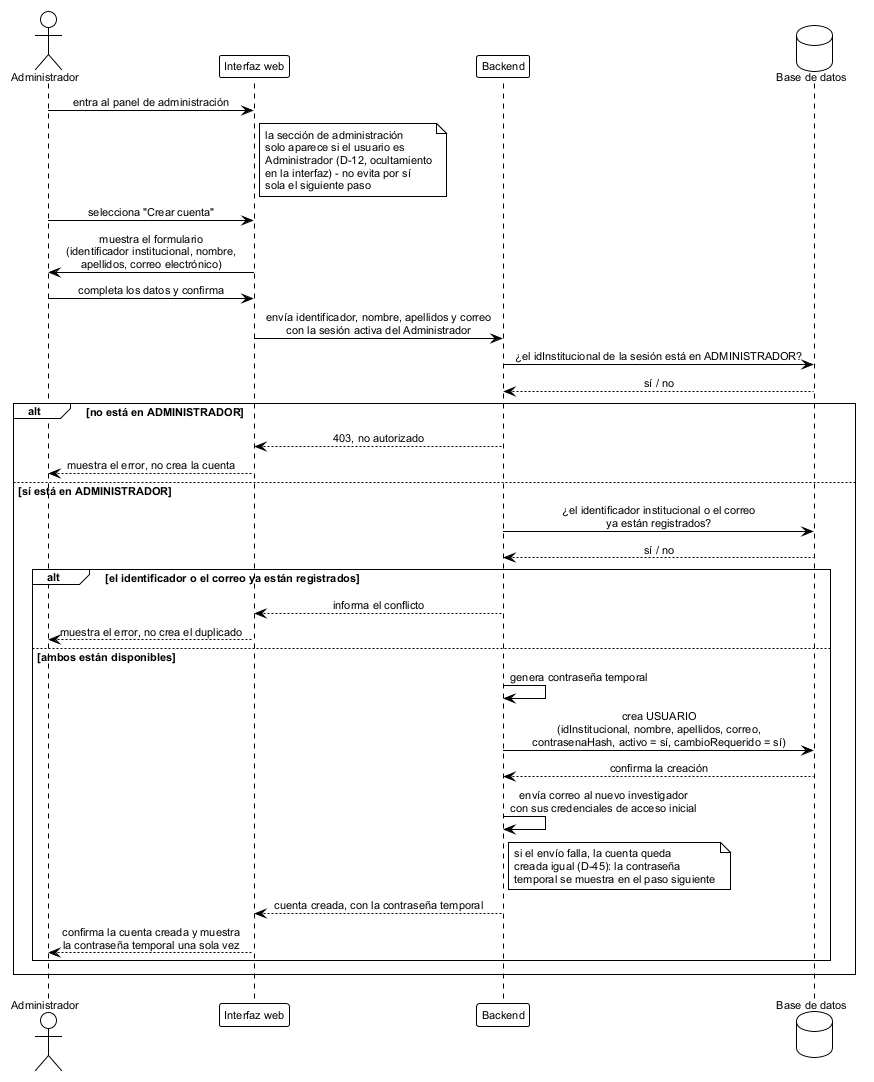
\includegraphics[width=\textwidth]{figures/mermaid/seq_crear_cuenta}
\caption{Secuencia: creación de cuenta de usuario por administrador [autoría propia].}
\label{fig:seq_registro}
\end{figure}

\begin{figure}[H]
\centering
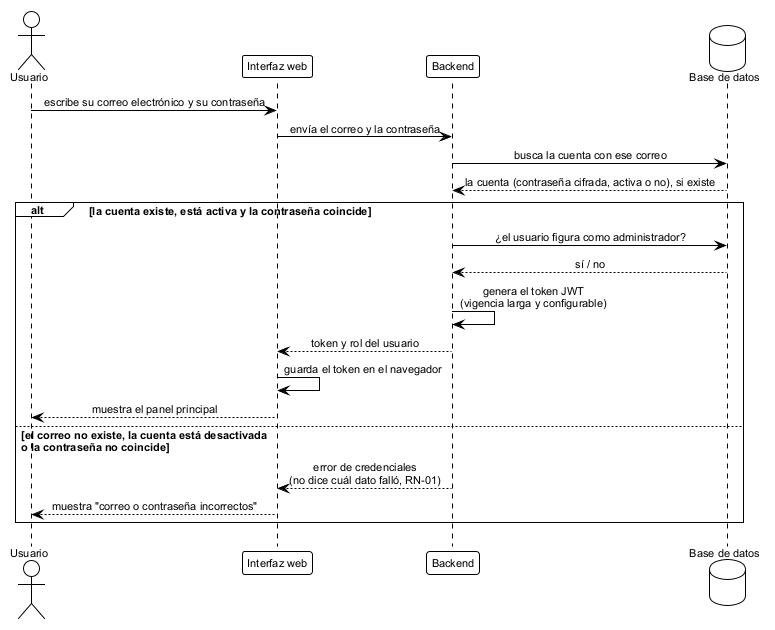
\includegraphics[width=\textwidth]{figures/mermaid/seq_login}
\caption{Secuencia: inicio de sesión (Investigador y Administrador) [autoría propia].}
\label{fig:seq_login}
\end{figure}

\begin{figure}[H]
\centering
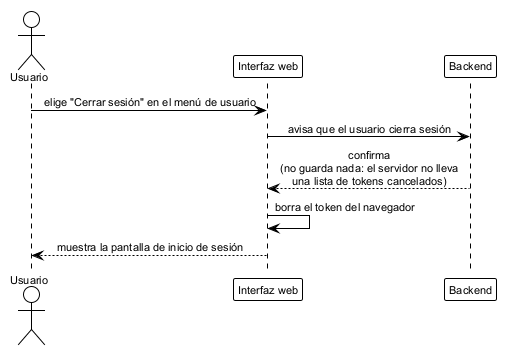
\includegraphics[width=\textwidth]{figures/mermaid/seq_logout}
\caption{Secuencia: cierre de sesión [autoría propia].}
\label{fig:seq_logout}
\end{figure}

\begin{figure}[H]
\centering
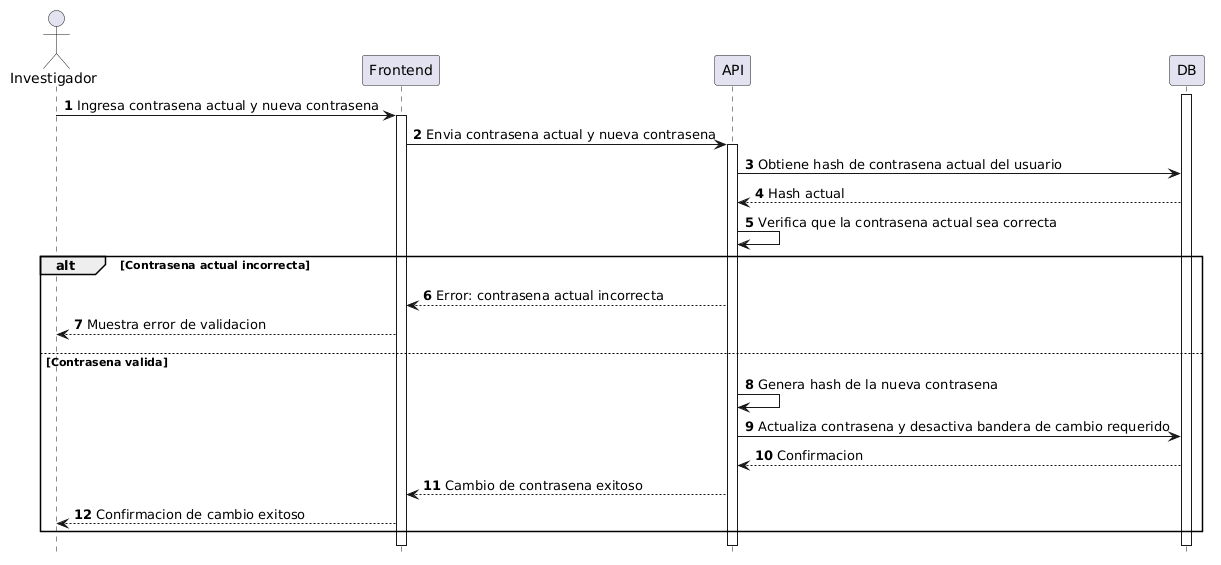
\includegraphics[width=\textwidth]{figures/mermaid/seq_cambio_pass_inv}
\caption{Secuencia: cambio de contraseña del usuario [autoría propia].}
\label{fig:seq_cambio_pass_inv}
\end{figure}

% ---- Paquete 5: Dashboard, notificaciones y administración ----

\subsection{Administración y perfil}

La gestión de usuarios (Figura~\ref{fig:seq_gestion_usuarios}) es exclusiva de
quien pertenece a \texttt{ADMINISTRADOR} (ver CU-15): permite crear cuentas
nuevas con contraseña temporal y desactivar cuentas existentes sin eliminarlas
(ver RF-05, RF-07). La configuración de perfil
(Figura~\ref{fig:seq_perfil}) está disponible para cualquier usuario con sesión
activa y permite actualizar nombre y correo electrónico.

\begin{figure}[H]
\centering
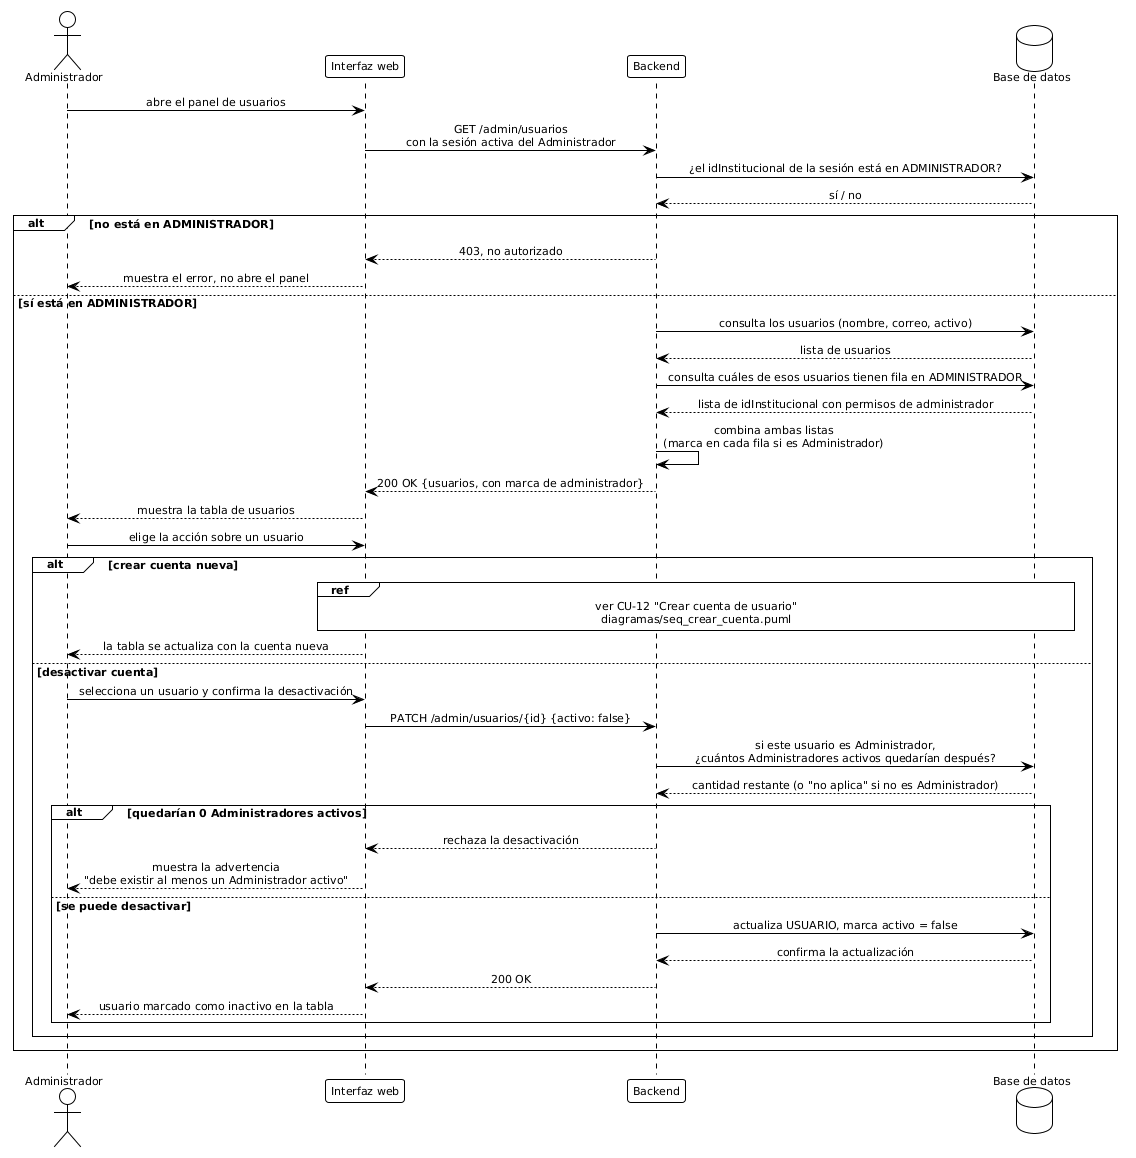
\includegraphics[width=\textwidth]{figures/mermaid/seq_gestion_usuarios}
\caption{Secuencia: gestión de usuarios por administrador (crear y desactivar) [autoría propia].}
\label{fig:seq_gestion_usuarios}
\end{figure}

\begin{figure}[H]
\centering
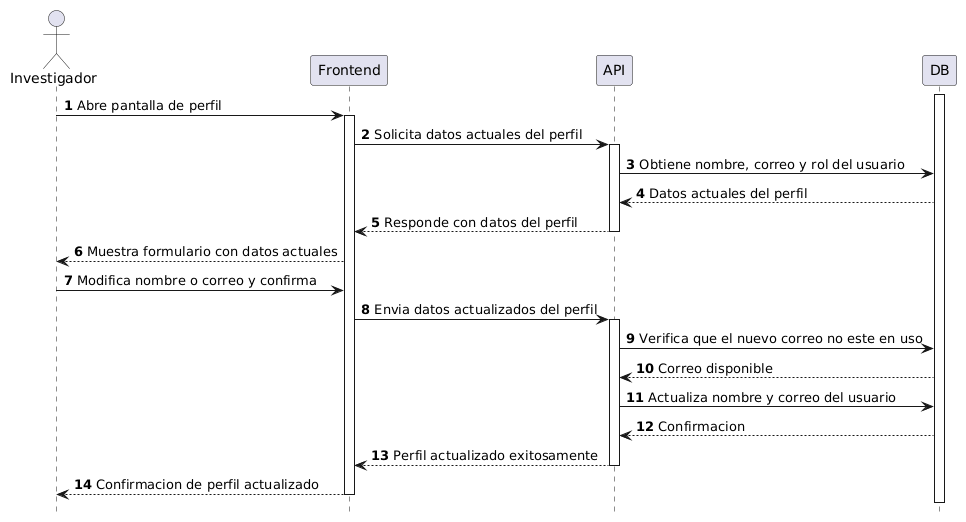
\includegraphics[width=\textwidth]{figures/mermaid/seq_perfil}
\caption{Secuencia: configuración de perfil del usuario [autoría propia].}
\label{fig:seq_perfil}
\end{figure}

% ---- Notificaciones ----

\subsection{Notificaciones}

El sistema genera notificaciones de forma automática cuando un análisis finaliza
(con o sin error) o cuando el espacio en disco supera el umbral de alerta (ver
RN-11, RNF-09). La Figura~\ref{fig:seq_notificaciones} muestra cómo el backend
persiste la notificación y cómo el frontend la consulta en el siguiente ciclo de
actualización.

\begin{figure}[H]
\centering
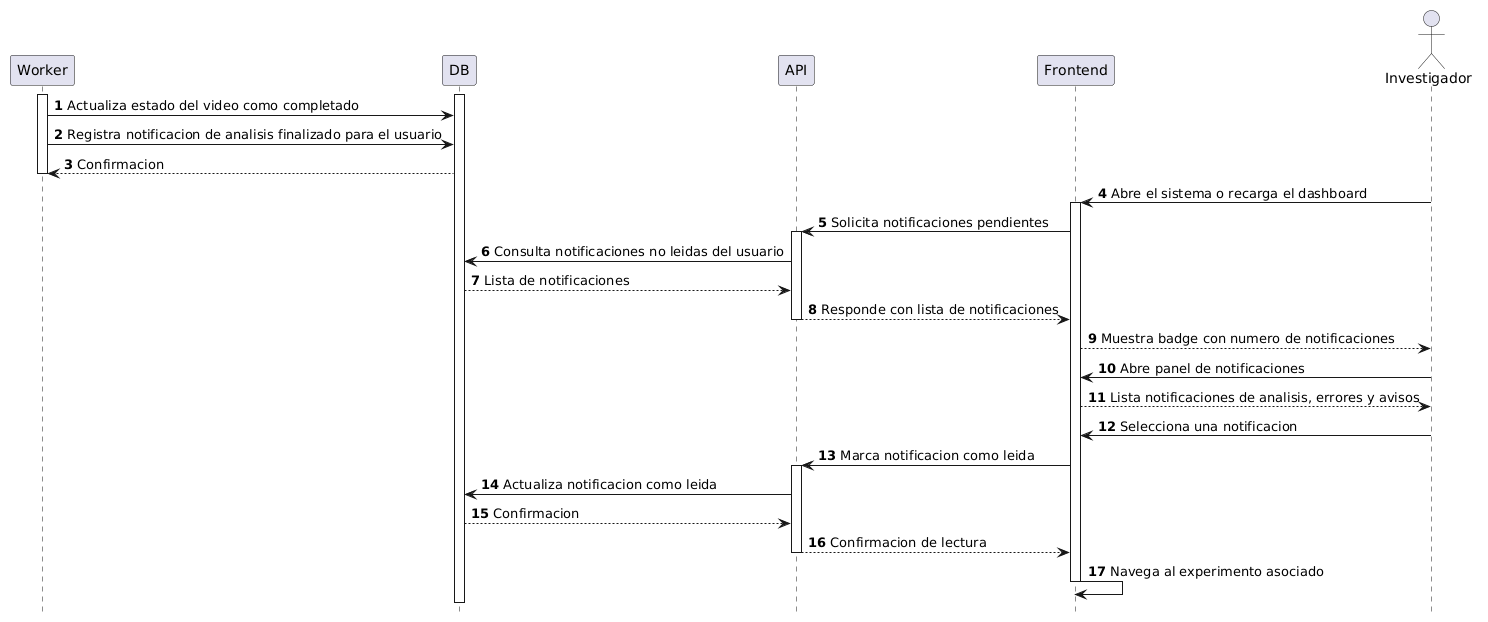
\includegraphics[width=\textwidth]{figures/mermaid/seq_notificaciones}
\caption{Secuencia: generación y consulta de notificaciones [autoría propia].}
\label{fig:seq_notificaciones}
\end{figure}

% ---- Paquetes 2, 3 y 4: Análisis, progreso, resultados y reportes ----

\subsection{Análisis, resultados y reportes}

Estos diagramas cubren el flujo central del sistema. La carga de video
(Figura~\ref{fig:seq_carga}) muestra cómo el investigador indica el grupo y
tratamiento, confirma la tanda sugerida por el sistema (D-19), sube el archivo y
el backend lo valida, lo registra y encola el análisis. El análisis automático
(Figura~\ref{fig:seq_analisis}) detalla la ejecución del pipeline por parte del
Worker: lectura del video, procesamiento en el módulo de visión por computadora y
almacenamiento de resultados. La consulta de progreso (Figura~\ref{fig:seq_progreso})
describe el mecanismo de \textit{polling} con el que el frontend verifica el
estado del análisis, incluyendo el camino alternativo cuando el video no se puede
procesar (no se abre o no se encuentran los cilindros, ver RN-11): el Worker genera
el reporte de diagnóstico PDF y lo pone disponible para descarga, sin necesidad de
un diagrama aparte para ese caso. Una vez completado el análisis, la consulta de
resultados (Figura~\ref{fig:seq_resultados}) devuelve los tiempos por espécimen
y conducta, y la descarga de reportes (Figura~\ref{fig:seq_reportes}) permite
exportar los datos en PDF, CSV o XLSX. Además, el usuario puede revisar el análisis
y corregir las etiquetas segundo a segundo (Figura~\ref{fig:seq_revision}; ver CU-25
a CU-27), lo que recalcula los totales por minuto.

\begin{figure}[H]
\centering
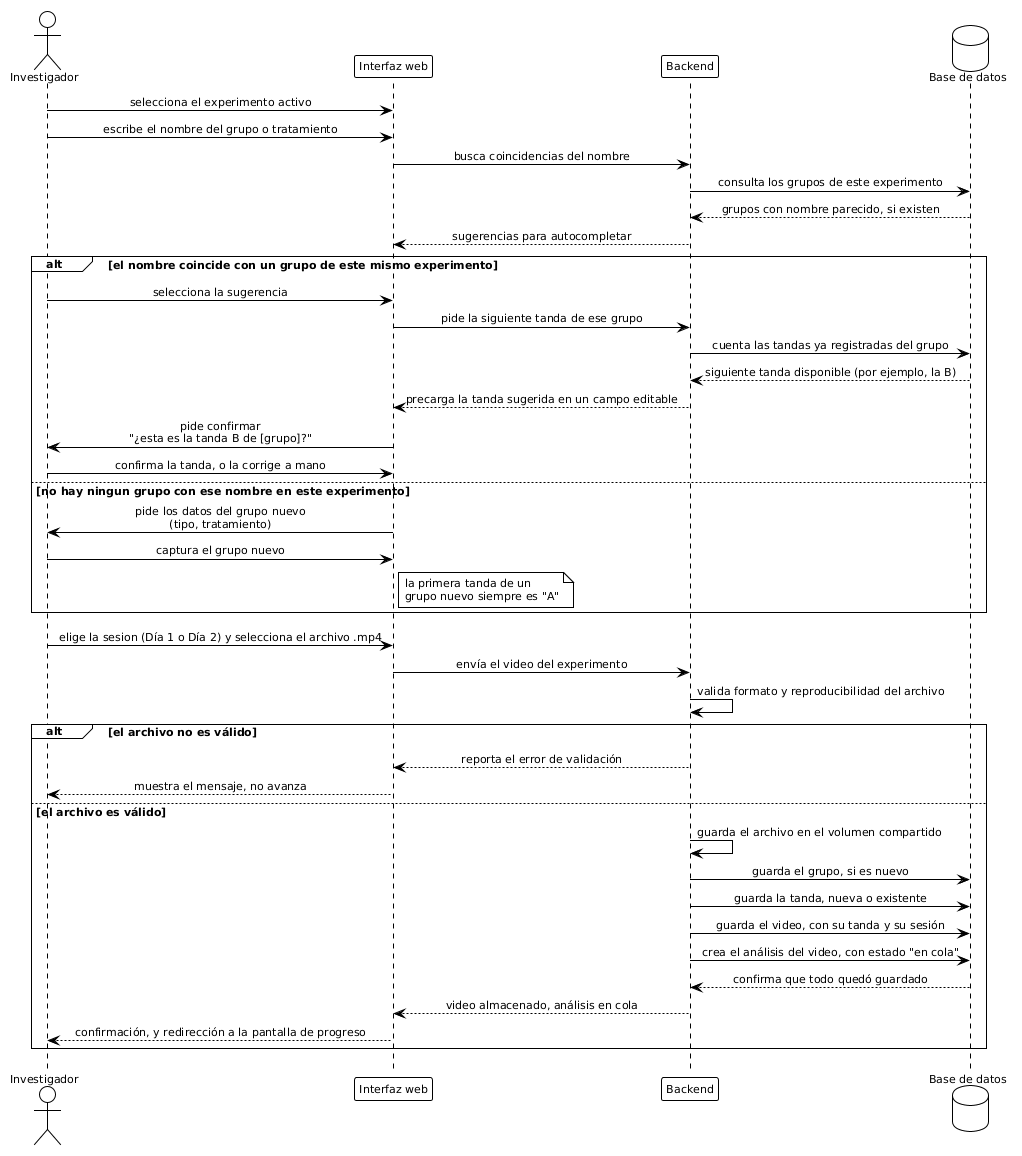
\includegraphics[width=\textwidth]{figures/mermaid/seq_carga_video}
\caption{Secuencia: carga de video con inferencia de tanda [autoría propia].}
\label{fig:seq_carga}
\end{figure}

\begin{figure}[H]
\centering
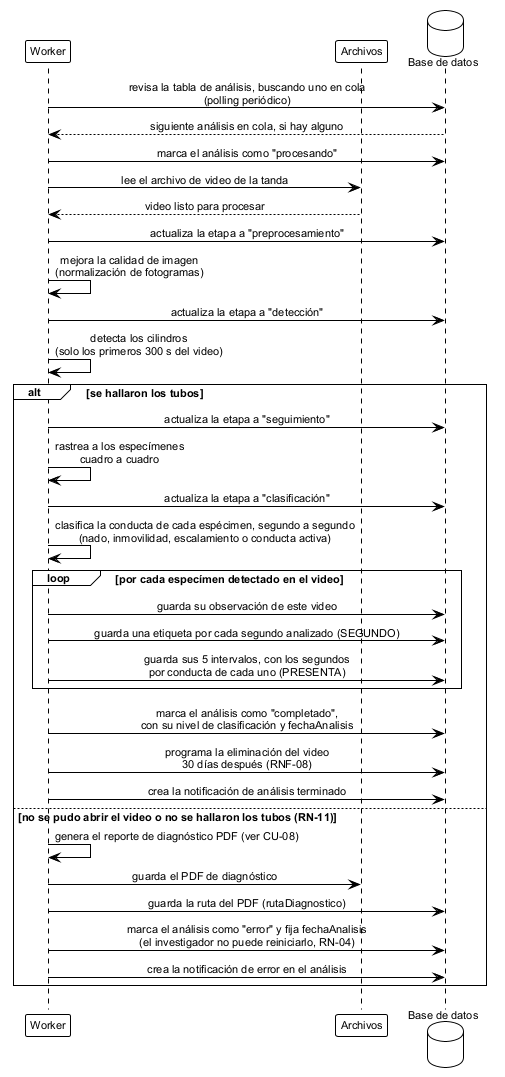
\includegraphics[width=\textwidth]{figures/mermaid/seq_analisis_automatico}
\caption{Secuencia: análisis automático (ejecución del pipeline por el Worker) [autoría propia].}
\label{fig:seq_analisis}
\end{figure}

\begin{figure}[H]
\centering
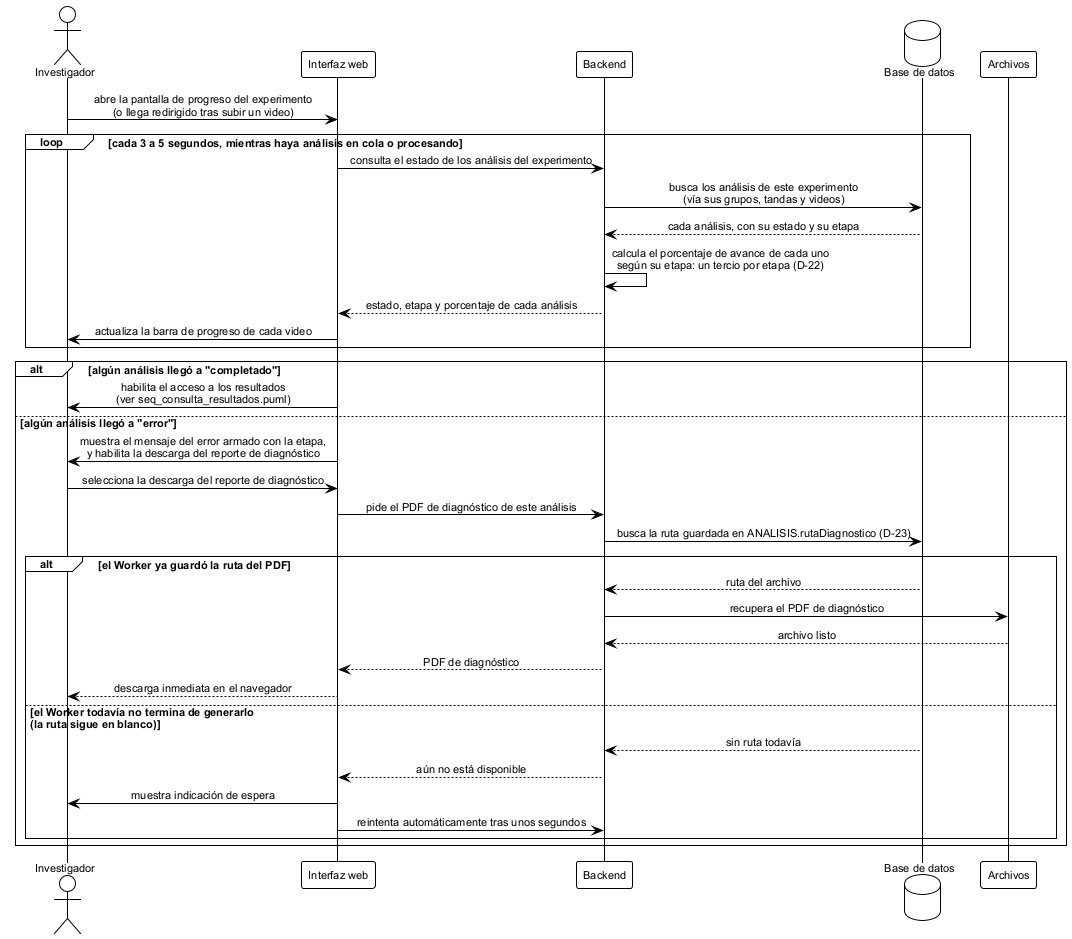
\includegraphics[width=\textwidth]{figures/mermaid/seq_consulta_progreso}
\caption{Secuencia: consulta de progreso del análisis, incluye manejo de error [autoría propia].}
\label{fig:seq_progreso}
\end{figure}

\begin{figure}[H]
\centering
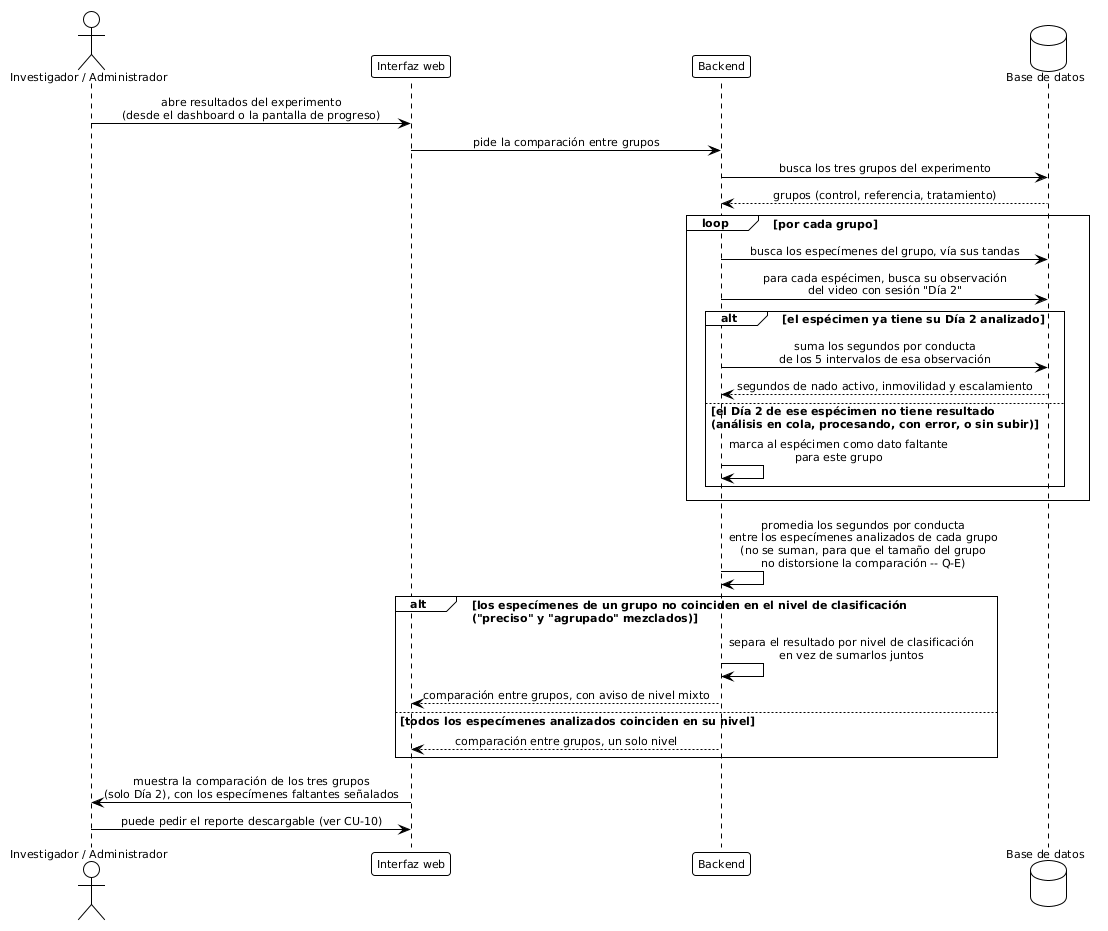
\includegraphics[width=\textwidth]{figures/mermaid/seq_consulta_resultados}
\caption{Secuencia: consulta de resultados del análisis [autoría propia].}
\label{fig:seq_resultados}
\end{figure}

\begin{figure}[H]
\centering
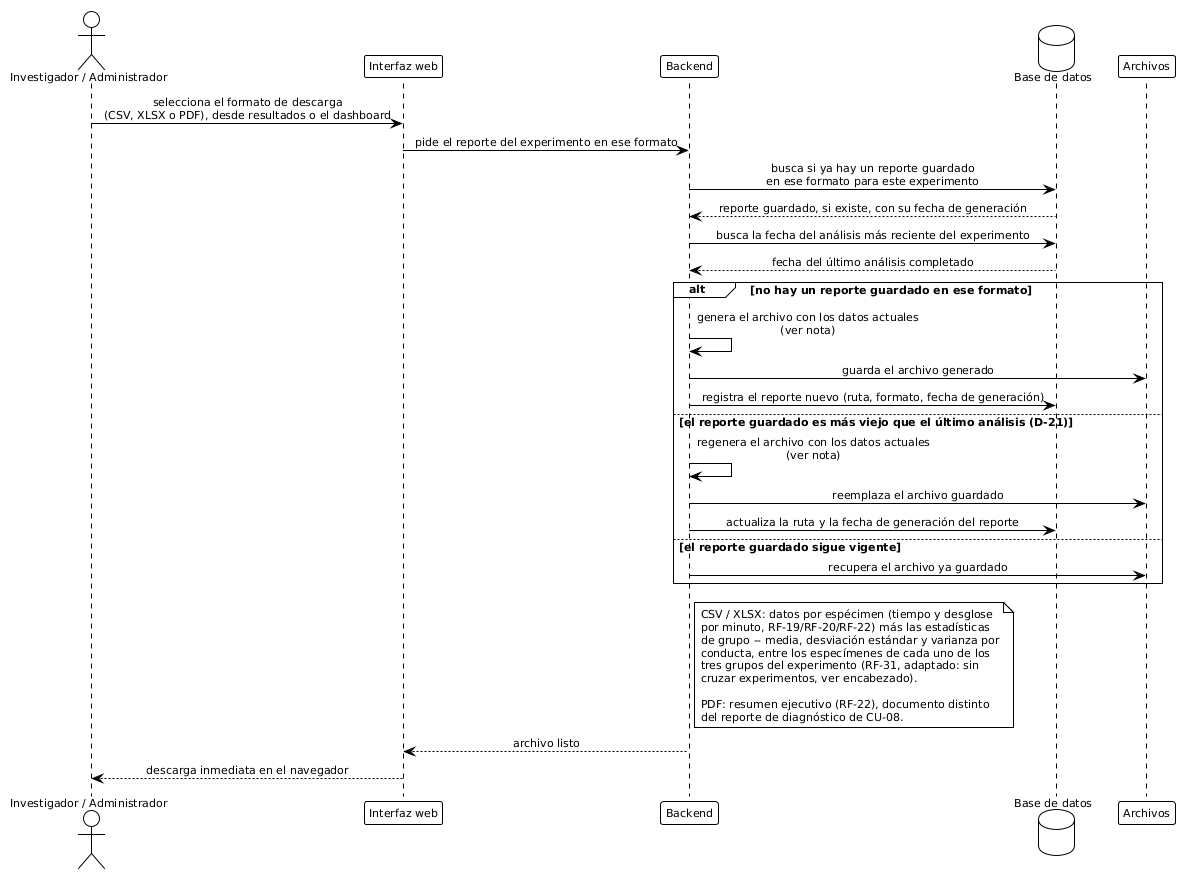
\includegraphics[width=\textwidth]{figures/mermaid/seq_descarga_reportes}
\caption{Secuencia: descarga de reportes (PDF, CSV, XLSX) [autoría propia].}
\label{fig:seq_reportes}
\end{figure}

\begin{figure}[H]
\centering
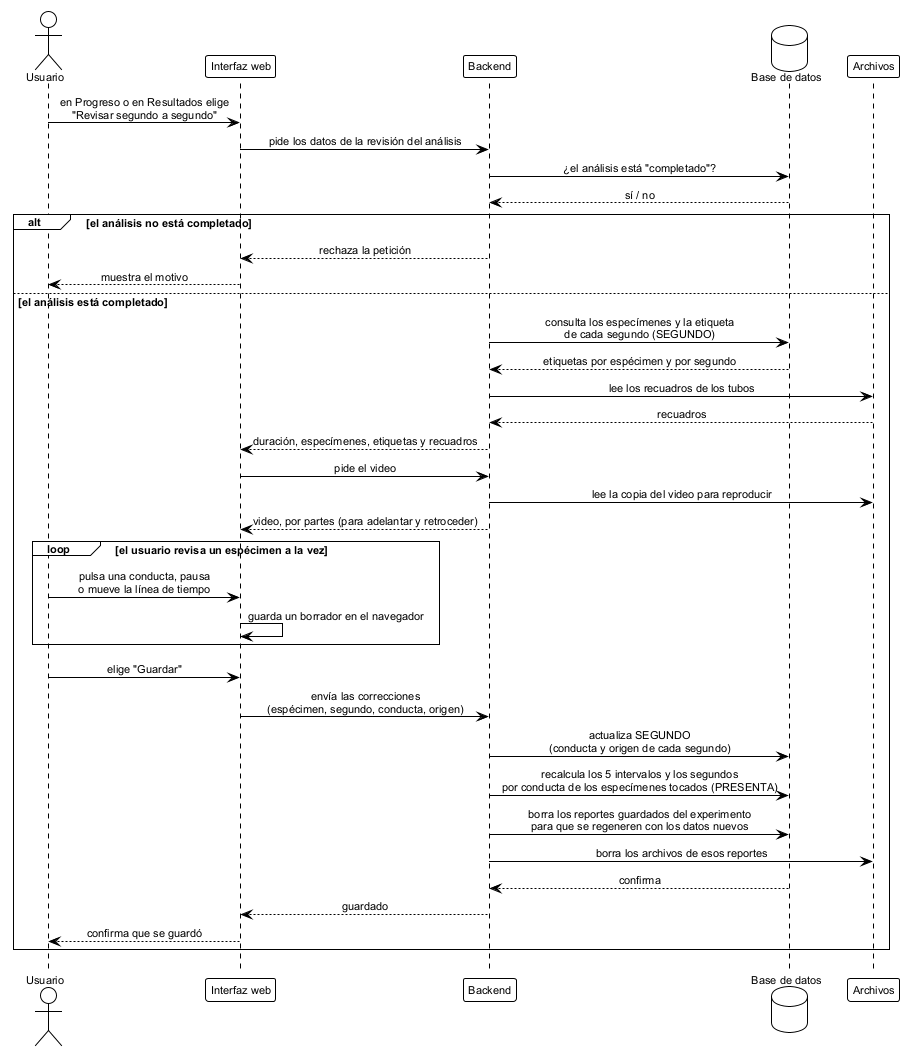
\includegraphics[width=\textwidth]{figures/mermaid/seq_revision_segundos}
\caption{Secuencia: revisión y corrección segundo a segundo [autoría propia].}
\label{fig:seq_revision}
\end{figure}

% -----------------------------------------------------------
\section{Diagrama de clases}
% -----------------------------------------------------------

El diagrama de clases \cite{omg_uml,iso42010} (Figura~\ref{fig:clases}) muestra
las entidades principales del dominio y sus relaciones desde la perspectiva del
backend. Las clases centrales del dominio experimental son \textbf{Usuario},
\textbf{Experimento}, \textbf{Grupo}, \textbf{Tanda}, \textbf{Especimen} y
\textbf{Video}: un experimento se compone de varios grupos (control, referencia,
tratamiento), cada grupo se graba en una o más tandas, cada tanda aloja de dos a
cuatro especímenes y produce uno o dos videos. \textbf{Administrador} hereda de
\textbf{Usuario} (D-08): no es un tipo de usuario aparte, sino un usuario con
permisos adicionales para gestionar cuentas y monitorear el sistema.

El pipeline de análisis se modela con dos clases de control: \textbf{Worker}, que
procesa la cola y elimina videos expirados, y \textbf{PipelineAnalisis}, que
ejecuta las tres etapas del análisis (preprocesamiento, localización de los
cilindros y clasificación) sobre cada \textbf{Video} y actualiza el \textbf{Analisis}
correspondiente. El modelo del clasificador y el umbral de confianza no son
clases del diagrama: son constantes del pipeline y no se registran por análisis.

Los resultados de conducta se modelan con \textbf{Observacion} (un espécimen
dentro de un video), \textbf{Intervalo} (cada minuto analizado) y la clase
asociativa \textbf{PRESENTA}, que vincula cada intervalo con las conductas del
catálogo \textbf{Conducta} y los segundos que ocupó cada una.

\begin{sidewaysfigure}
\centering
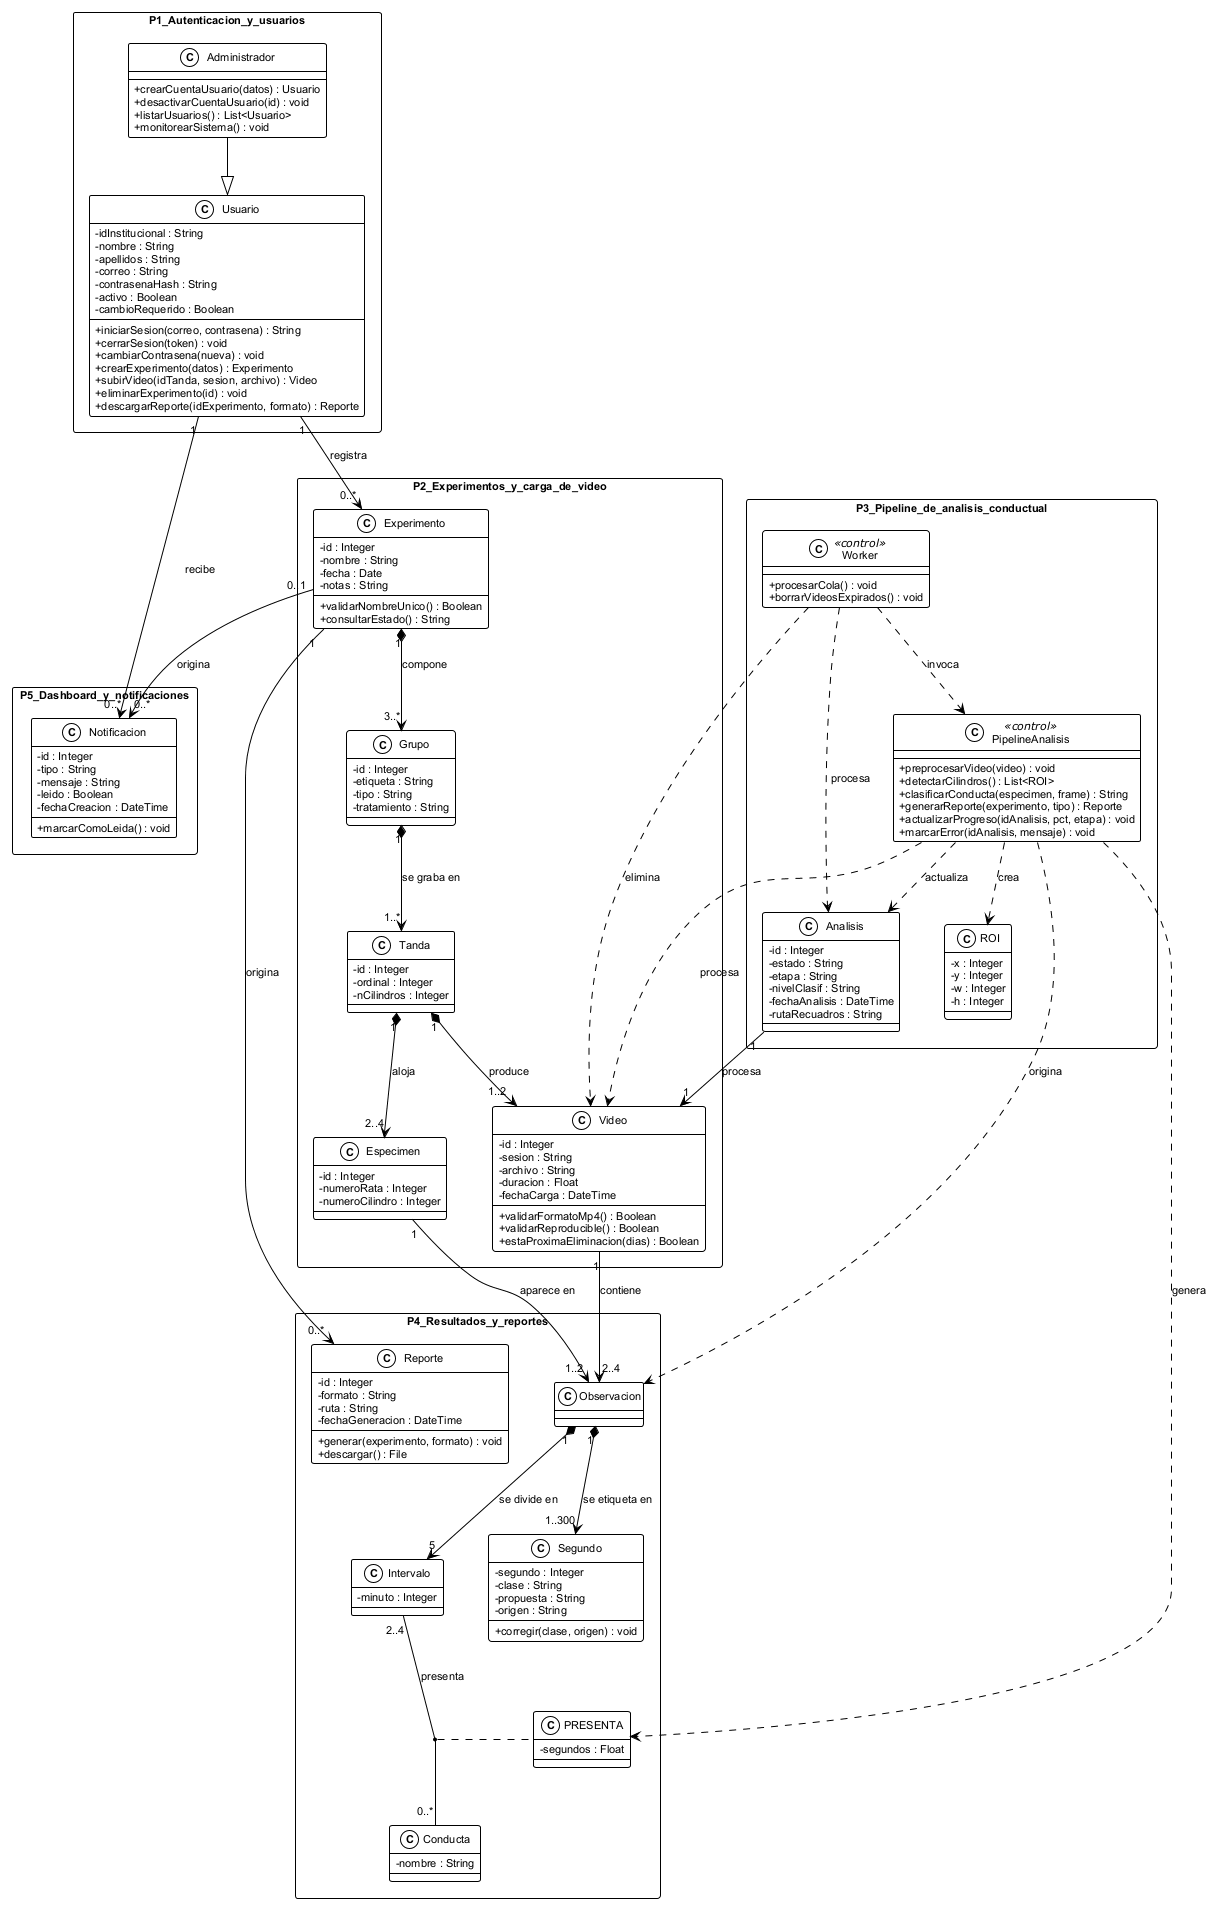
\includegraphics[width=\textheight, height=\textwidth, keepaspectratio]{diagramas/clases}
\caption{Diagrama de clases del sistema [autoría propia].}
\label{fig:clases}
\end{sidewaysfigure}
% -----------------------------------------------------------
\section{Diseño de la interfaz web}
% -----------------------------------------------------------

La interfaz tiene once pantallas, diseñadas para que un investigador sin
experiencia en programación pueda completar el flujo completo ---crear experimento,
esperar el análisis, consultar y descargar resultados--- sin necesitar asistencia
técnica (ver RNF-06). Las capturas de esta sección corresponden a la segunda versión
de los mockups (v2), construida con datos de ejemplo y sin conexión al servidor.

\subsection{Pantalla de inicio de sesión}

Formulario con campos de correo electrónico y contraseña. Las credenciales
incorrectas muestran un mensaje de error genérico sin revelar cuál campo falló
(ver RN-01). Incluye enlace de recuperación de contraseña (RF-03). Antes de enviar
las credenciales, la pantalla comprueba que el correo tenga un formato válido.

\begin{figure}[H]
\centering
  \begin{subfigure}[t]{0.48\textwidth}
    \centering
    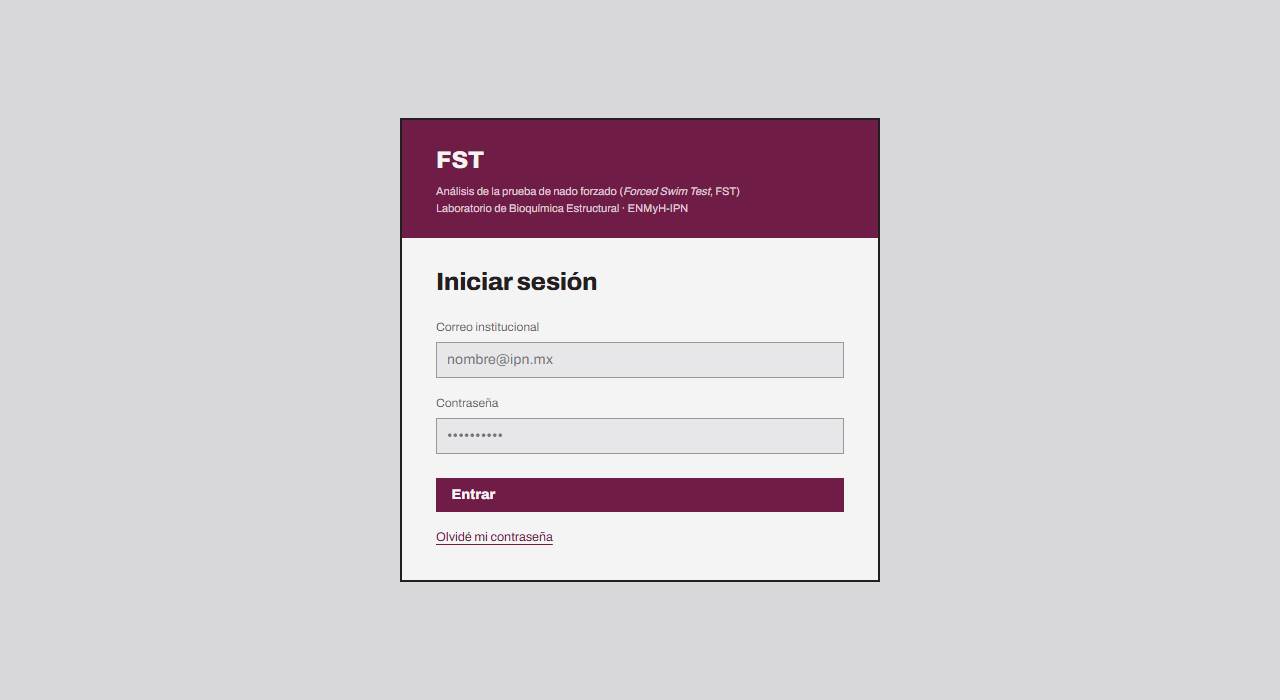
\includegraphics[width=\textwidth]{figures/mockups/v2/login}
    \caption{Estado normal.}
    \label{fig:ui_login_normal}
  \end{subfigure}
  \hfill
  \begin{subfigure}[t]{0.48\textwidth}
    \centering
    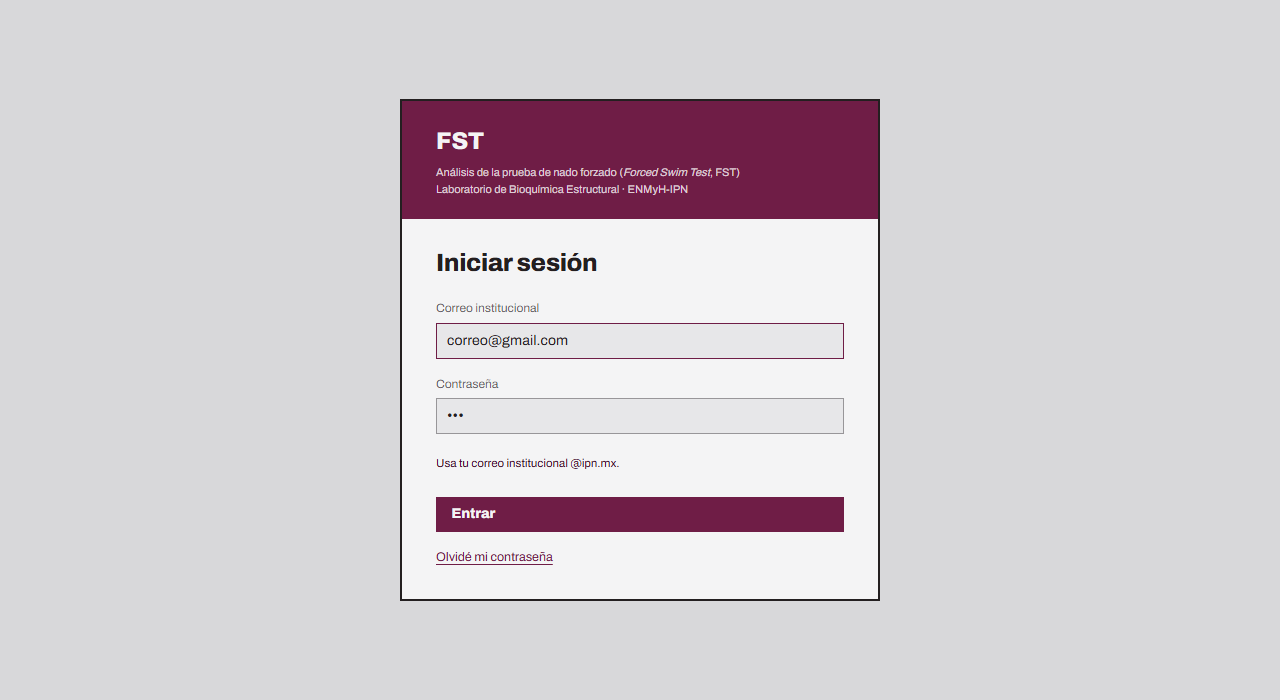
\includegraphics[width=\textwidth]{figures/mockups/v2/estados/login_error}
    \caption{Credenciales incorrectas (RN-01).}
    \label{fig:ui_login_error}
  \end{subfigure}
\caption{Pantalla de inicio de sesión [autoría propia].}
\label{fig:ui_login}
\end{figure}

\subsection{Primer acceso y perfil}

Una cuenta creada por el Administrador entra con una contraseña temporal y, mientras
no la cambie, no tiene acceso a ninguna otra pantalla (RF-05, RF-07). Después, el
investigador puede consultar sus datos y cambiar su contraseña desde la pantalla de
perfil; el identificador institucional es de solo lectura.

\begin{figure}[H]
\centering
  \begin{subfigure}[t]{0.48\textwidth}
    \centering
    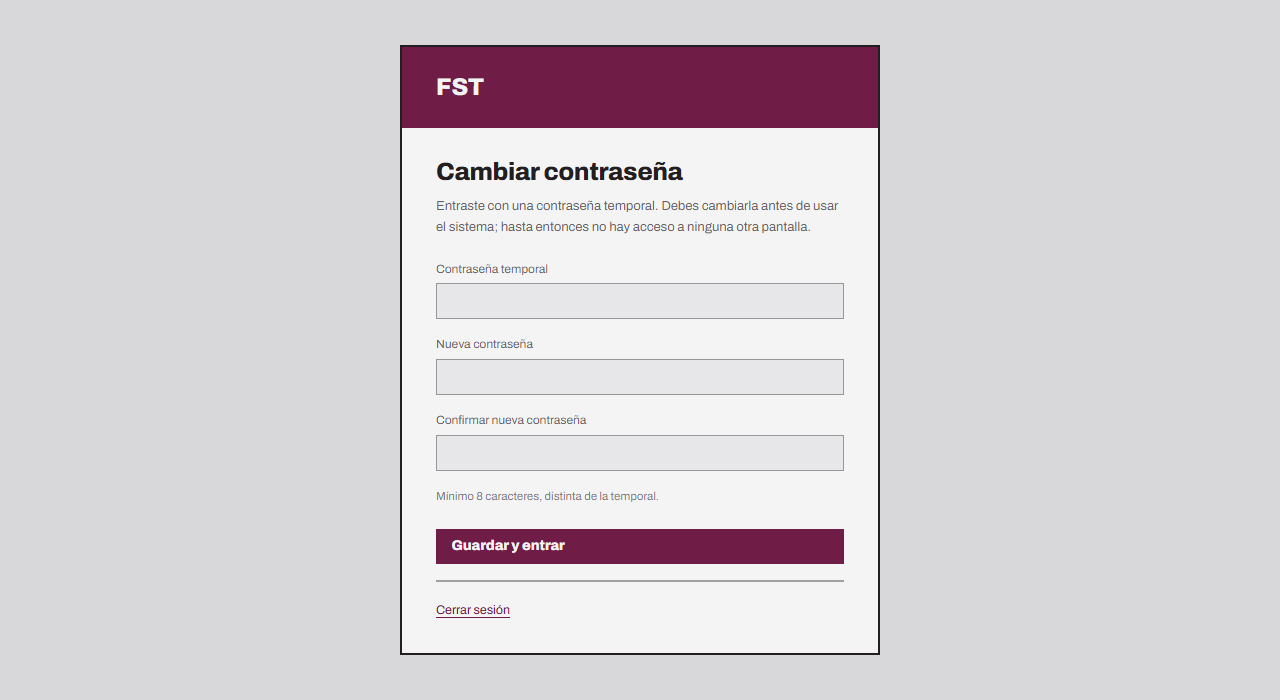
\includegraphics[width=\textwidth]{figures/mockups/v2/primer-acceso}
    \caption{Cambio obligatorio de la contraseña temporal.}
    \label{fig:ui_primer_acceso}
  \end{subfigure}
  \hfill
  \begin{subfigure}[t]{0.48\textwidth}
    \centering
    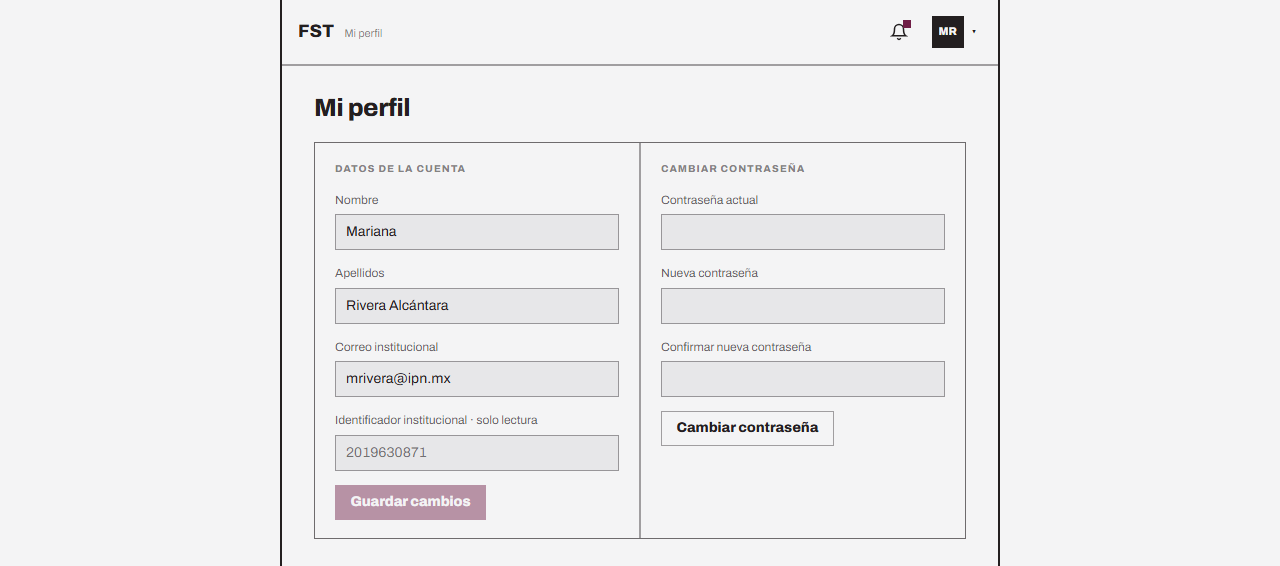
\includegraphics[width=\textwidth]{figures/mockups/v2/perfil}
    \caption{Perfil del usuario.}
    \label{fig:ui_perfil}
  \end{subfigure}
\caption{Primer acceso y perfil [autoría propia].}
\label{fig:ui_perfil_acceso}
\end{figure}

\subsection{Lista de experimentos}

Lista de experimentos del laboratorio con grupos, especímenes, videos del Día~2,
estado, responsable, retención y acceso al reporte (ver RN-08). Muestra un aviso
cuando un video está a menos de 7~días de ser eliminado automáticamente (RF-24).
Incluye filtros por estado y búsqueda por nombre o tratamiento. La eliminación de un
experimento no está en esta lista sino en su detalle.

\begin{figure}[H]
\centering
  \begin{subfigure}[t]{0.48\textwidth}
    \centering
    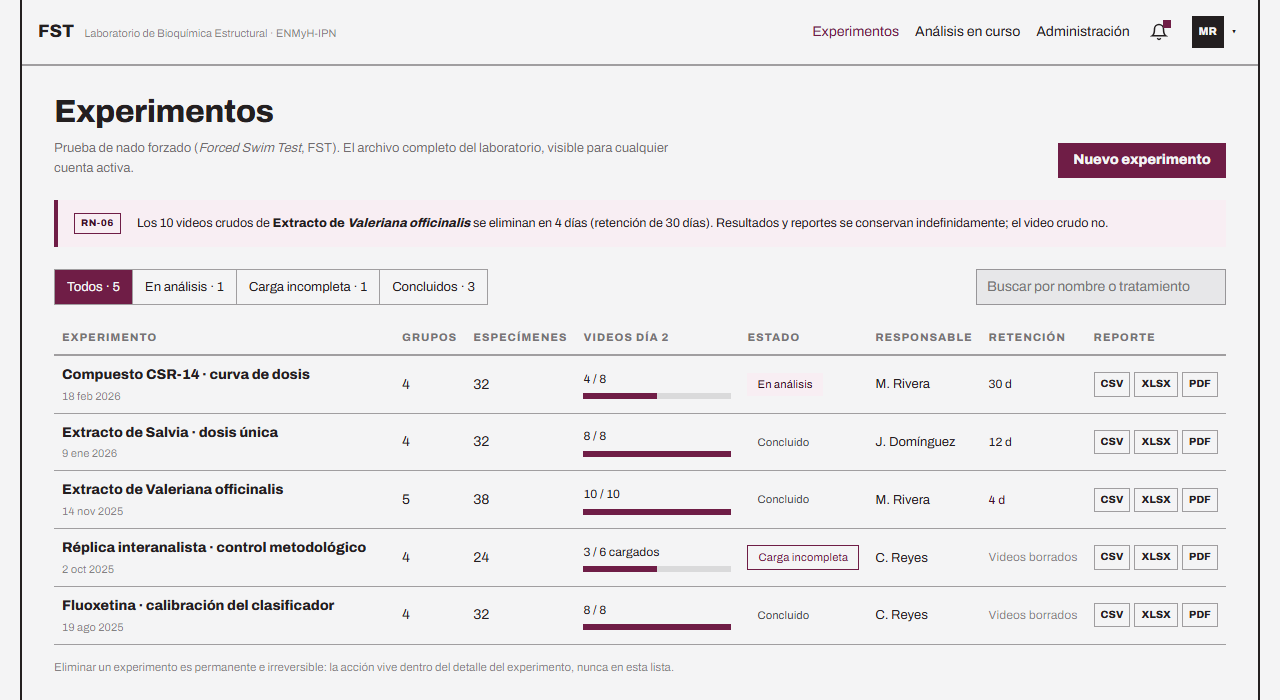
\includegraphics[width=\textwidth]{figures/mockups/v2/experimentos}
    \caption{Lista con experimentos y aviso de vencimiento (RF-24).}
    \label{fig:ui_dashboard_normal}
  \end{subfigure}
  \hfill
  \begin{subfigure}[t]{0.48\textwidth}
    \centering
    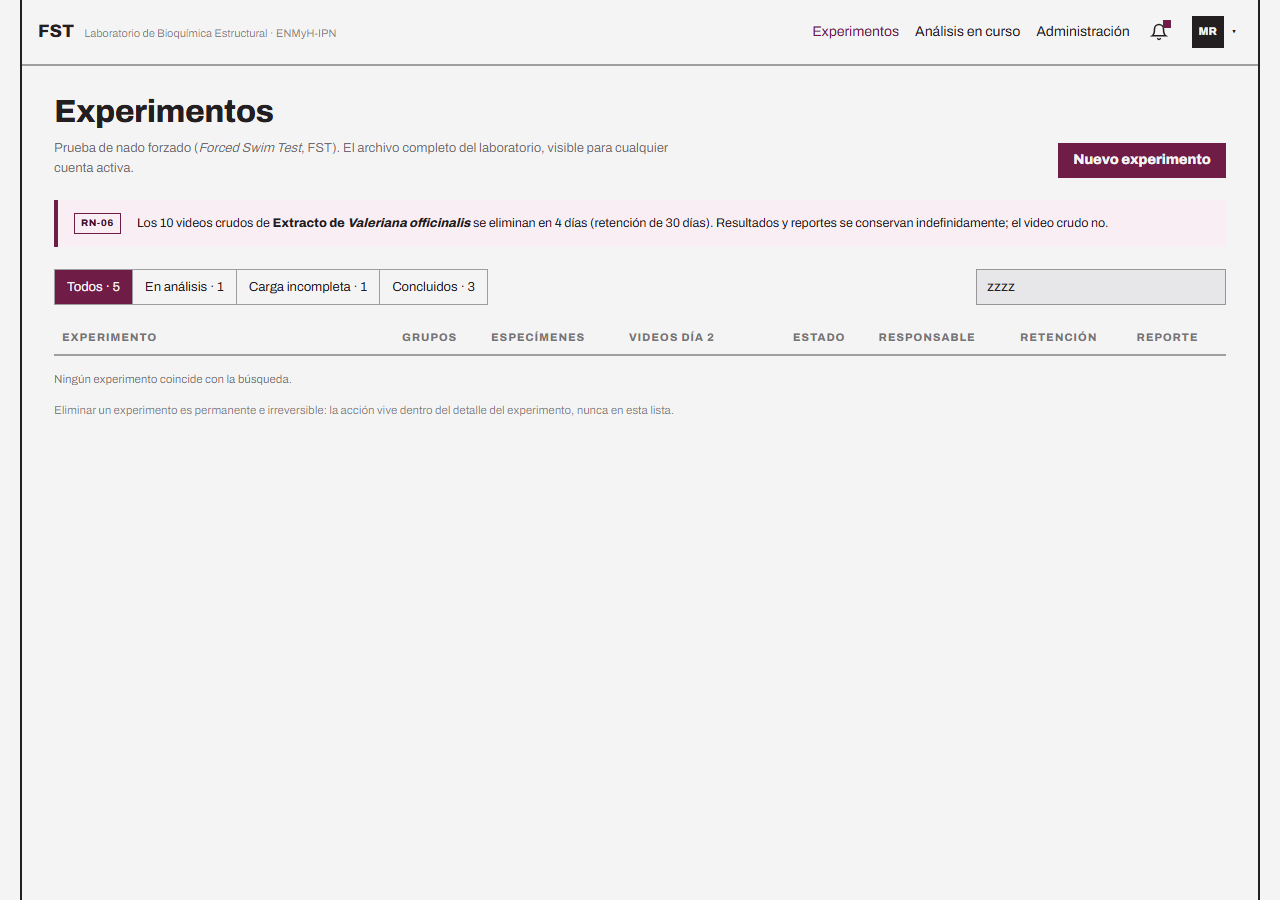
\includegraphics[width=\textwidth]{figures/mockups/v2/estados/experimentos_vacio}
    \caption{Búsqueda sin coincidencias.}
    \label{fig:ui_dashboard_vacio}
  \end{subfigure}
\caption{Lista de experimentos del investigador [autoría propia].}
\label{fig:ui_dashboard}
\end{figure}

\subsection{Detalle de experimento y de grupo}

El detalle de un experimento reúne sus grupos y el estado de cada tanda. Solo quien
creó el experimento o un administrador puede eliminarlo, y la acción pide escribir el
nombre del experimento y la contraseña (RF-27, RN-09). El detalle de un grupo muestra
sus tandas, los especímenes de cada una con el cilindro que ocuparon y los videos de
Día~1 y Día~2 con su estado.

\begin{figure}[H]
\centering
  \begin{subfigure}[t]{0.48\textwidth}
    \centering
    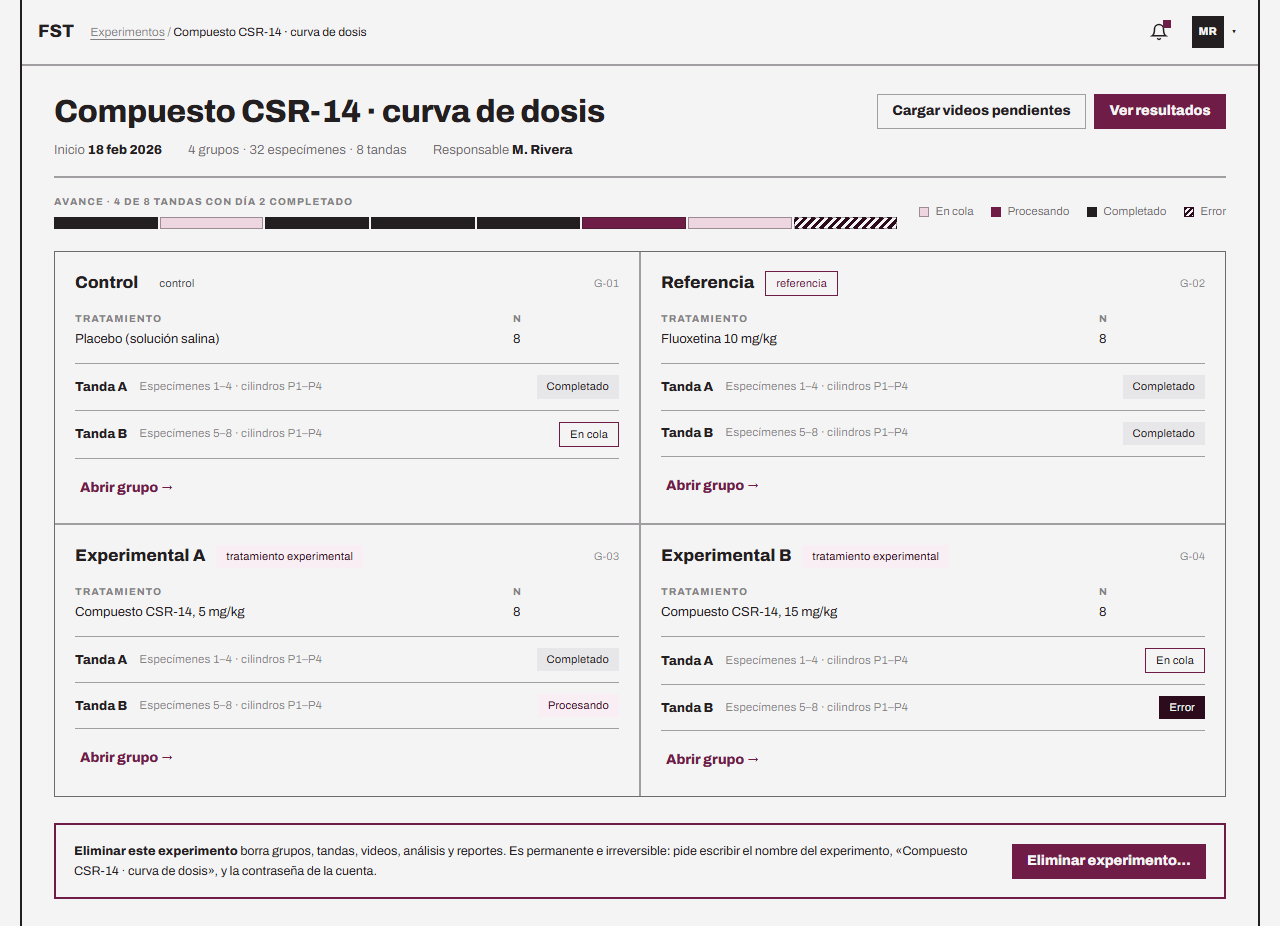
\includegraphics[width=\textwidth]{figures/mockups/v2/experimento}
    \caption{Detalle de un experimento.}
    \label{fig:ui_experimento}
  \end{subfigure}
  \hfill
  \begin{subfigure}[t]{0.48\textwidth}
    \centering
    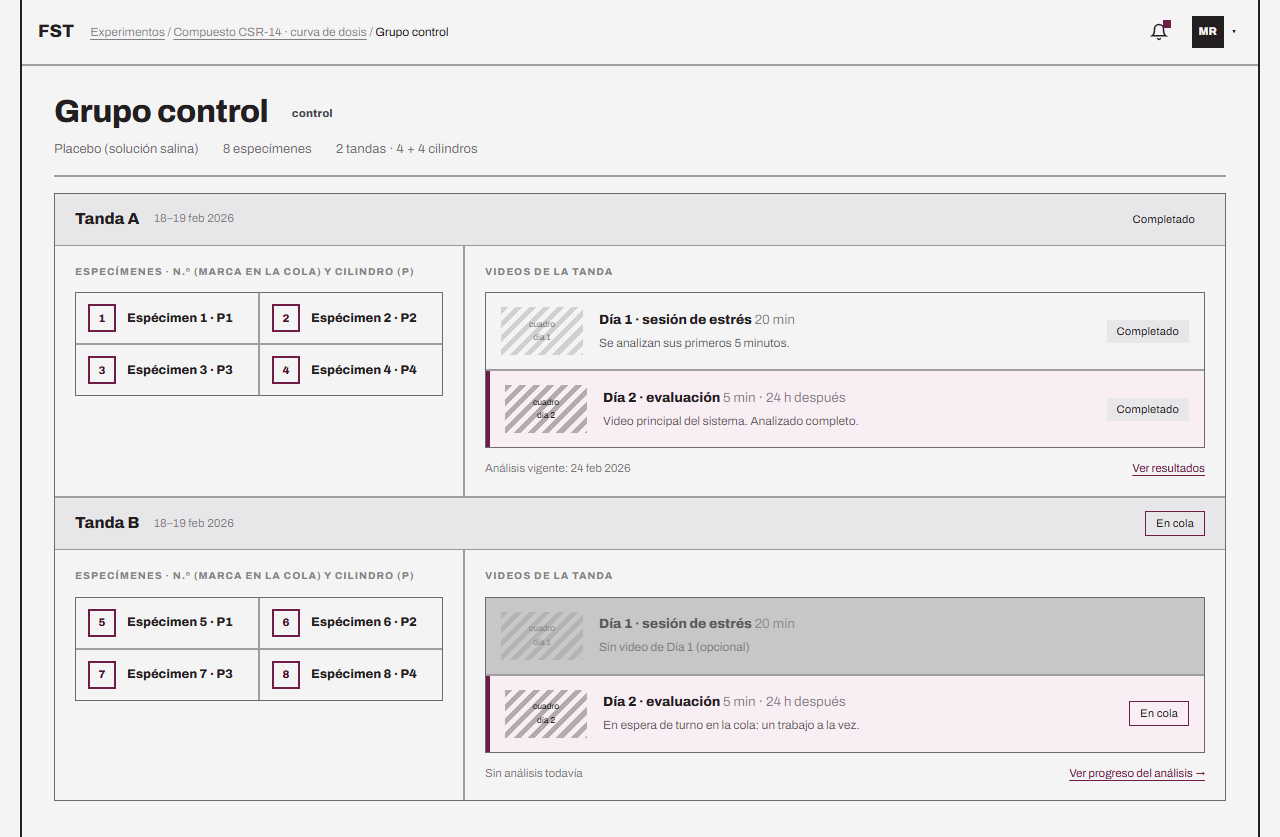
\includegraphics[width=\textwidth]{figures/mockups/v2/grupo}
    \caption{Detalle de un grupo.}
    \label{fig:ui_grupo}
  \end{subfigure}
\caption{Detalle de experimento y de grupo [autoría propia].}
\label{fig:ui_detalle}
\end{figure}

\subsection{Creación de experimento y carga de video}

Formulario en dos pasos: datos generales del experimento (nombre, fecha y notas, ver
CU-04); y carga del video de una tanda, donde se indica el grupo o tratamiento, la
tanda sugerida por el sistema y sujeta a confirmación (ver CU-05, D-19), de dos a
cuatro cilindros en el cuadro, la sesión (Día~1 o Día~2) y el archivo. Solo acepta
archivos \texttt{.mp4} o \texttt{.mov} en horizontal; el rechazo de formato ocurre en
el cliente antes de iniciar la subida. Una vez completada la carga válida, el
análisis inicia automáticamente (RF-12). El segundo paso se repite cada vez que
se agrega una nueva tanda al experimento, no ocurre una sola vez.

La división en pasos se eligió sobre un formulario único porque la carga de video
puede tardar varios minutos según el tamaño del archivo: separar los datos
del experimento de la carga de cada tanda permite que el investigador corrija un
nombre o fecha sin necesidad de volver a subir un video, y permite agregar tandas
nuevas más adelante sin repetir los datos del experimento.

\begin{figure}[H]
\centering
  \begin{subfigure}[t]{0.48\textwidth}
    \centering
    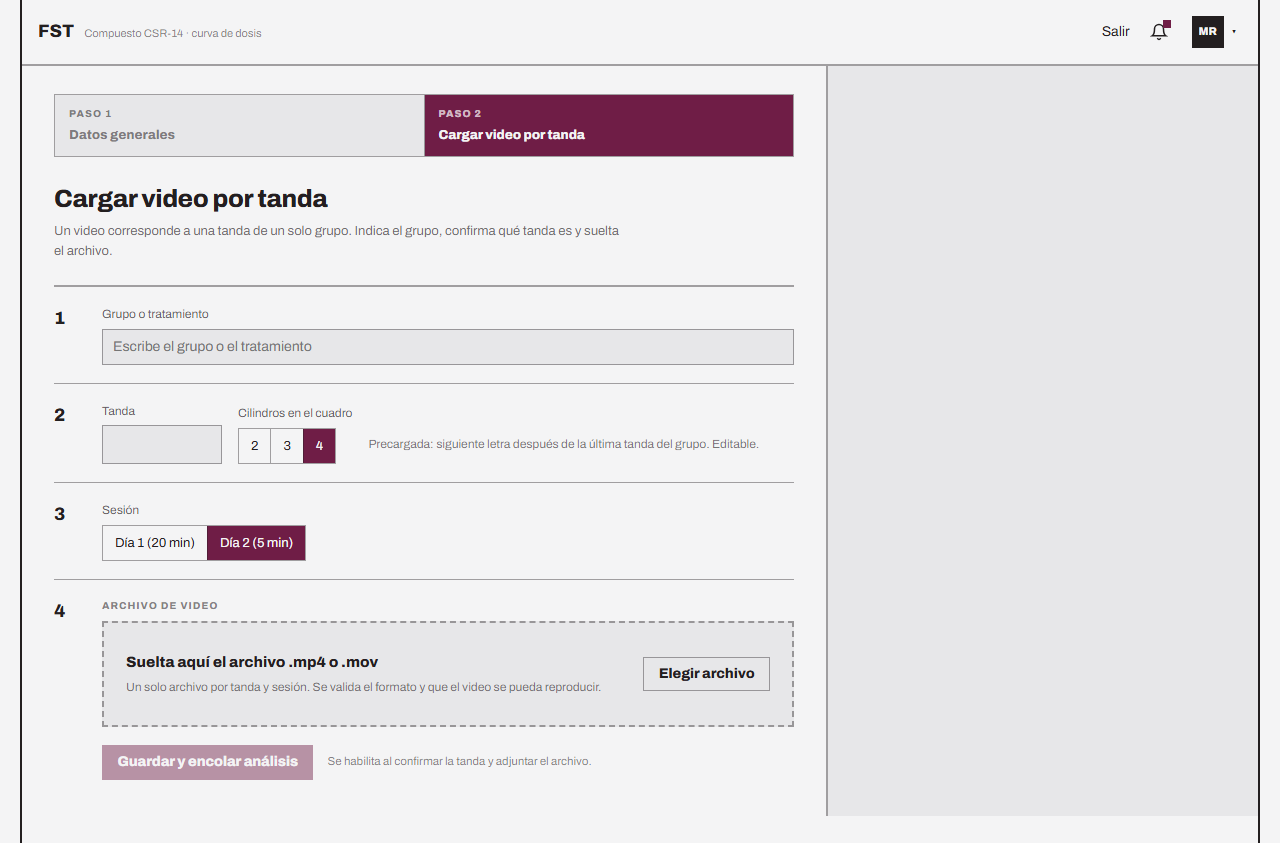
\includegraphics[width=\textwidth]{figures/mockups/v2/cargar-video}
    \caption{Formulario vacío (paso 2).}
    \label{fig:ui_nuevo_vacio}
  \end{subfigure}
  \hfill
  \begin{subfigure}[t]{0.48\textwidth}
    \centering
    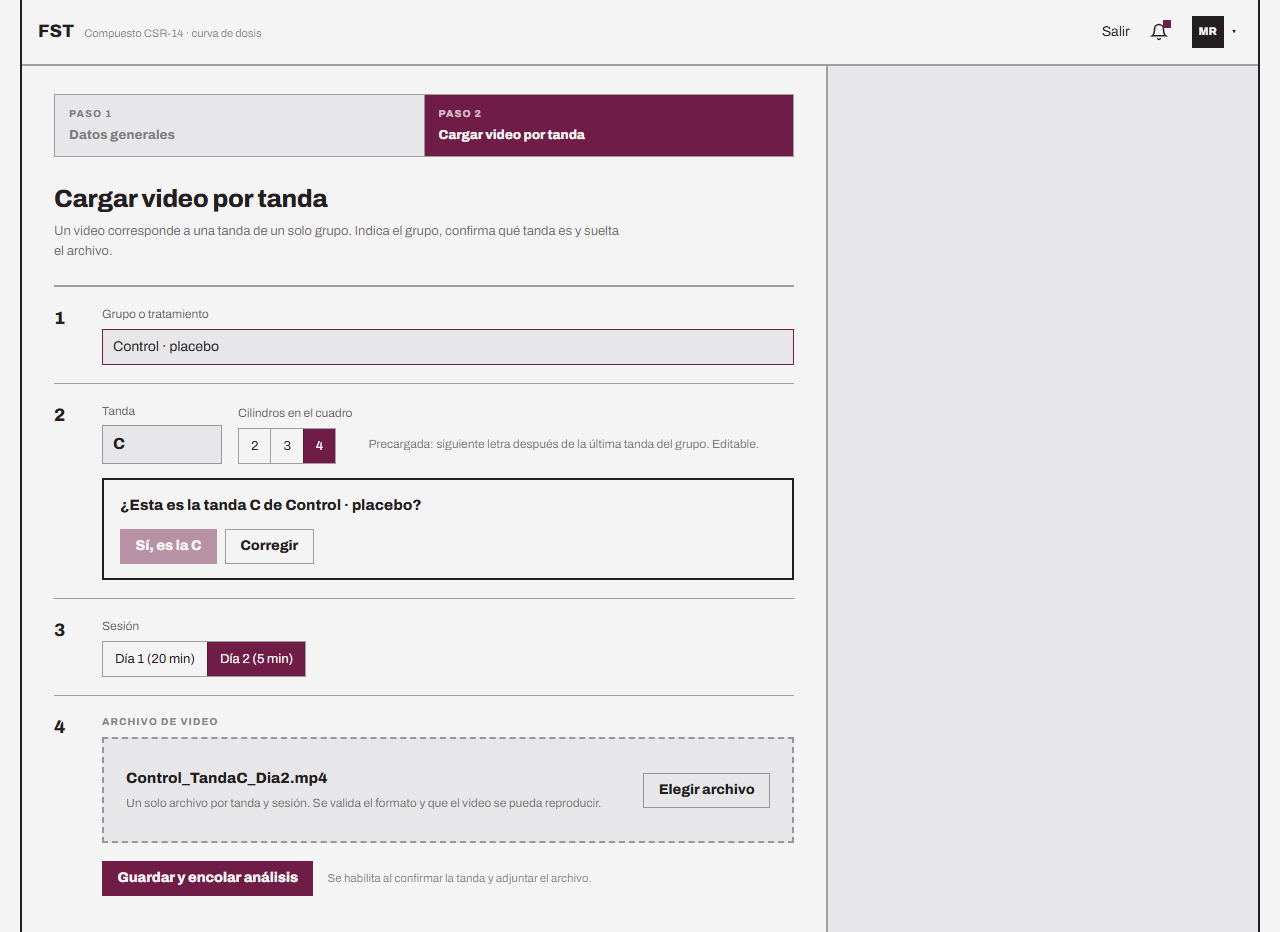
\includegraphics[width=\textwidth]{figures/mockups/v2/estados/cargar_lleno}
    \caption{Grupo, tanda confirmada y archivo seleccionado.}
    \label{fig:ui_nuevo_lleno}
  \end{subfigure}

  \vspace{8pt}
  \begin{subfigure}[t]{0.48\textwidth}
    \centering
    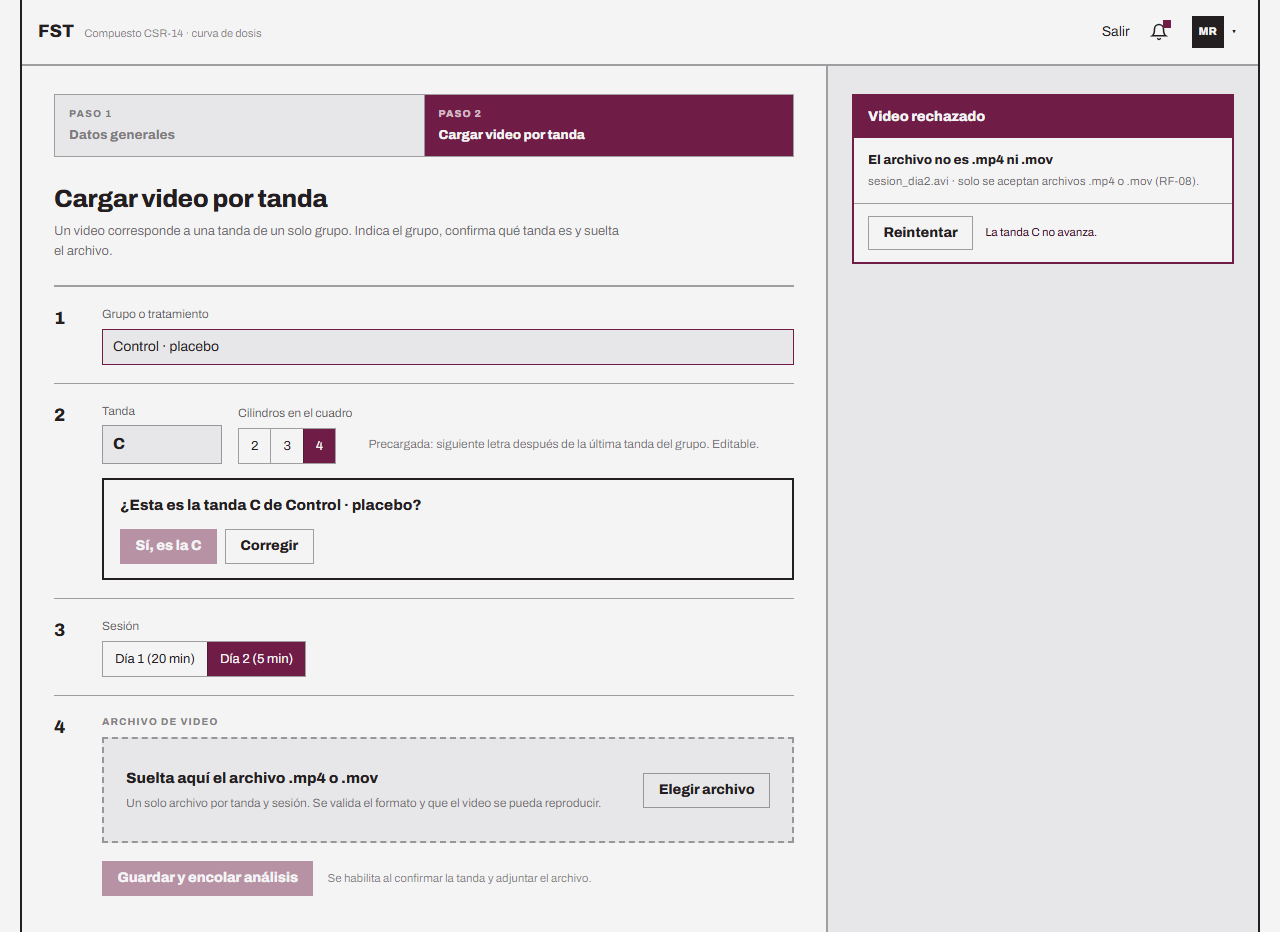
\includegraphics[width=\textwidth]{figures/mockups/v2/estados/cargar_error_formato}
    \caption{Archivo rechazado por formato (RF-08).}
    \label{fig:ui_nuevo_error}
  \end{subfigure}
  \hfill
  \begin{subfigure}[t]{0.48\textwidth}
    \centering
    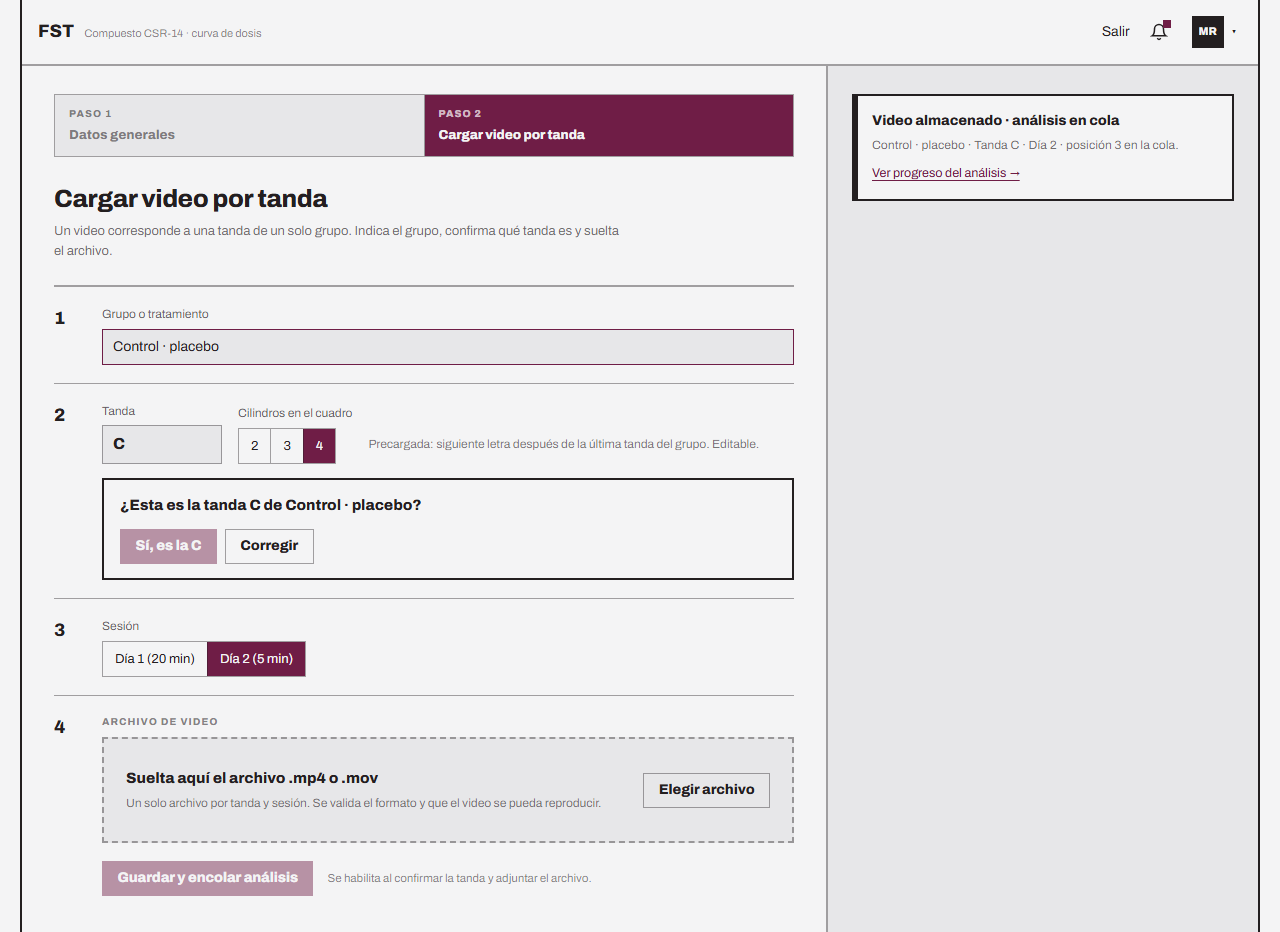
\includegraphics[width=\textwidth]{figures/mockups/v2/estados/cargar_exito}
    \caption{Carga exitosa, análisis en cola (RF-12).}
    \label{fig:ui_nuevo_exito}
  \end{subfigure}
\caption{Pantalla de carga de video por tanda [autoría propia].}
\label{fig:ui_nuevo}
\end{figure}

\subsection{Progreso del análisis}

Muestra el estado actual del pipeline con las tres etapas (preprocesamiento,
localización de los cilindros y clasificación) y una barra de progreso en
porcentaje. Si ocurre un error, muestra la descripción, según la etapa en que se
detuvo, y el botón de descarga del reporte de diagnóstico (RF-16). Los errores definidos son dos: el video
no se pudo abrir o no se encontraron los cilindros. Cuando un análisis se completa,
la pantalla habilita «Ver resultados» y «Revisar segundo a segundo». Debajo lista la
cola de trabajos. El análisis continúa aunque el investigador cierre la pestaña (RF-15).

No hay botón de cancelar visible durante el análisis. La decisión fue deliberada: el
laboratorio no tiene casos de uso donde cancele un análisis a mitad de camino, y
agregar la funcionalidad implicaría manejar el estado de cancelación en el worker y
limpiar los archivos parciales. Si en el futuro surge esa necesidad, el endpoint
\texttt{POST /experiments/\{id\}/groups/\{grupo\}/videos} puede extenderse para
soportar cancelación.

\begin{figure}[H]
\centering
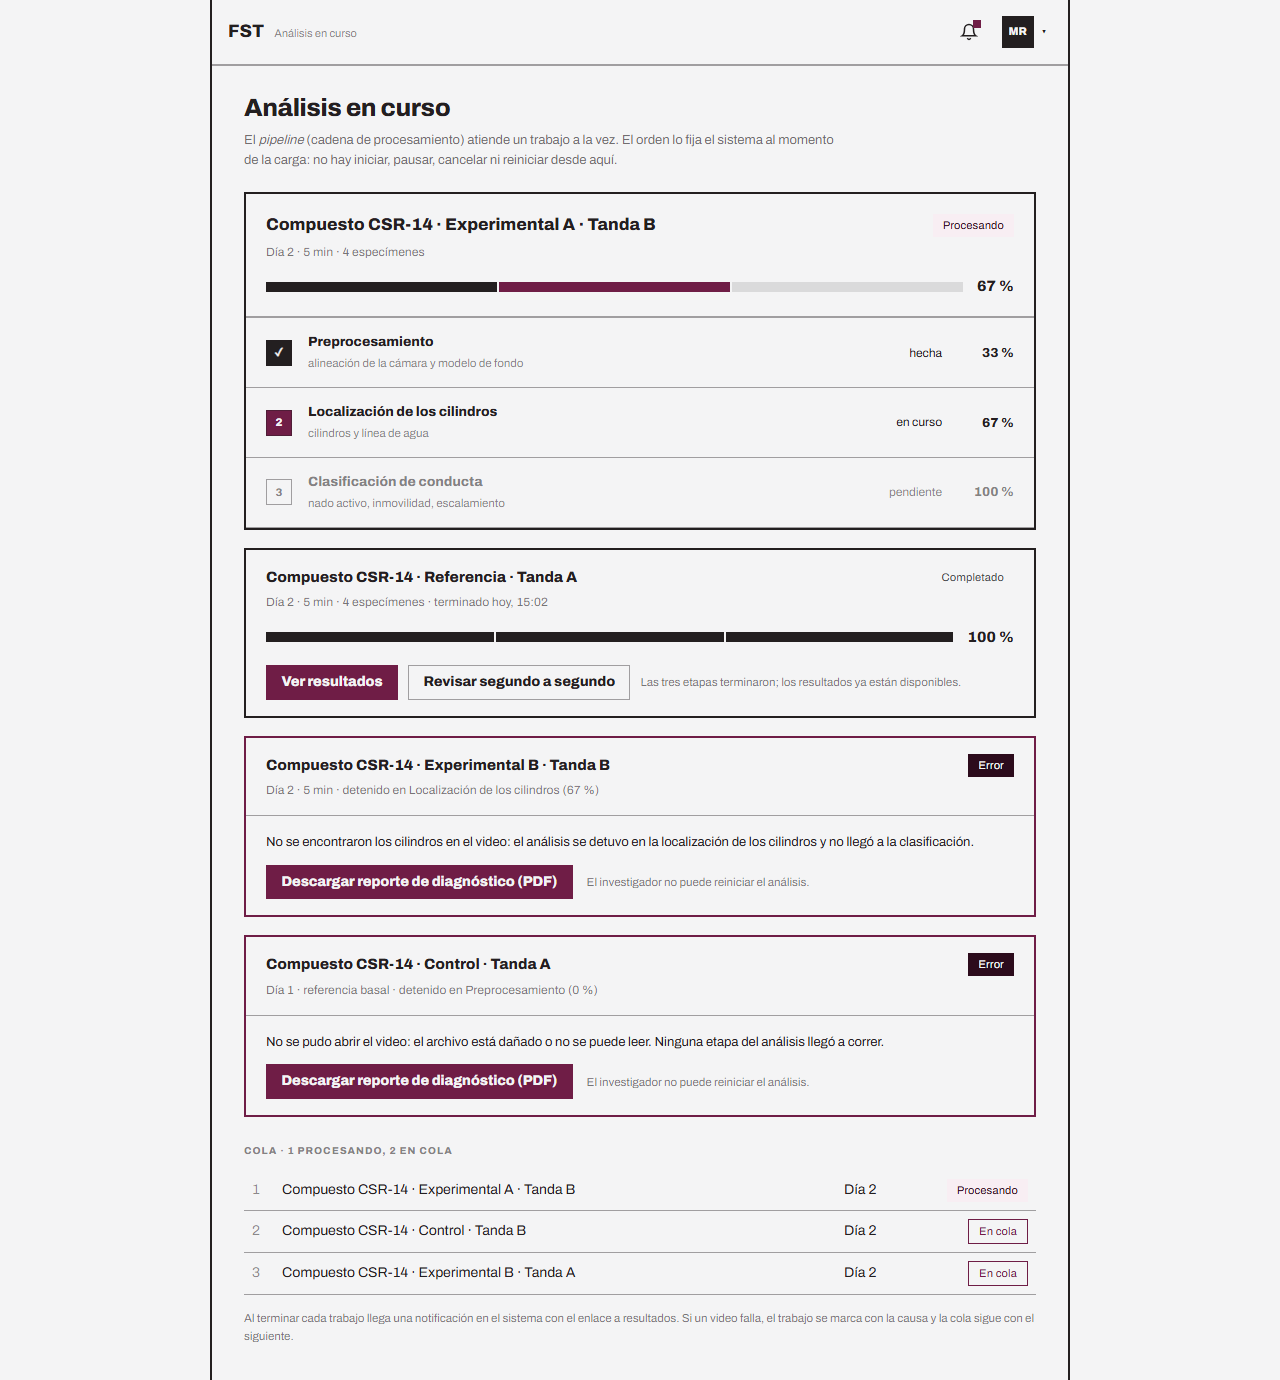
\includegraphics[width=0.75\textwidth]{figures/mockups/v2/progreso}
\caption{Pantalla de progreso del análisis: un análisis en curso, uno completado con acceso a resultados y a la revisión, dos detenidos por error ---cilindros no detectados y video que no se pudo abrir--- (RF-16) y la cola de trabajos [autoría propia].}
\label{fig:ui_progreso}
\end{figure}

\subsection{Resultados del experimento}

Cuatro pestañas: resultados por espécimen, comparación entre grupos, línea de tiempo
por minuto (RF-20) y bloques de 5~s (RF-18), donde cada bloque muestra la conducta con
más segundos y, dentro, los cinco segundos que lo componen, para notar las conductas
breves y comparar con el análisis manual. La vista por espécimen
muestra el tiempo por conducta con media, desviación estándar y varianza (RF-19), el
nivel de clasificación del análisis y la leyenda de conductas; en el panel lateral
se compara la inmovilidad entre los grupos con los videos del Día~2 (RF-21). Esa
comparación promedia los segundos por espécimen de cada grupo y señala los especímenes
cuyo video aún no está analizado, que no entran al promedio (RN-12). Si un grupo mezcla
análisis en nivel preciso y agrupado, los muestra por separado. Incluye botones de
descarga en PDF, CSV y XLSX.

\begin{figure}[H]
\centering
  \begin{subfigure}[t]{0.508\textwidth}
    \centering
    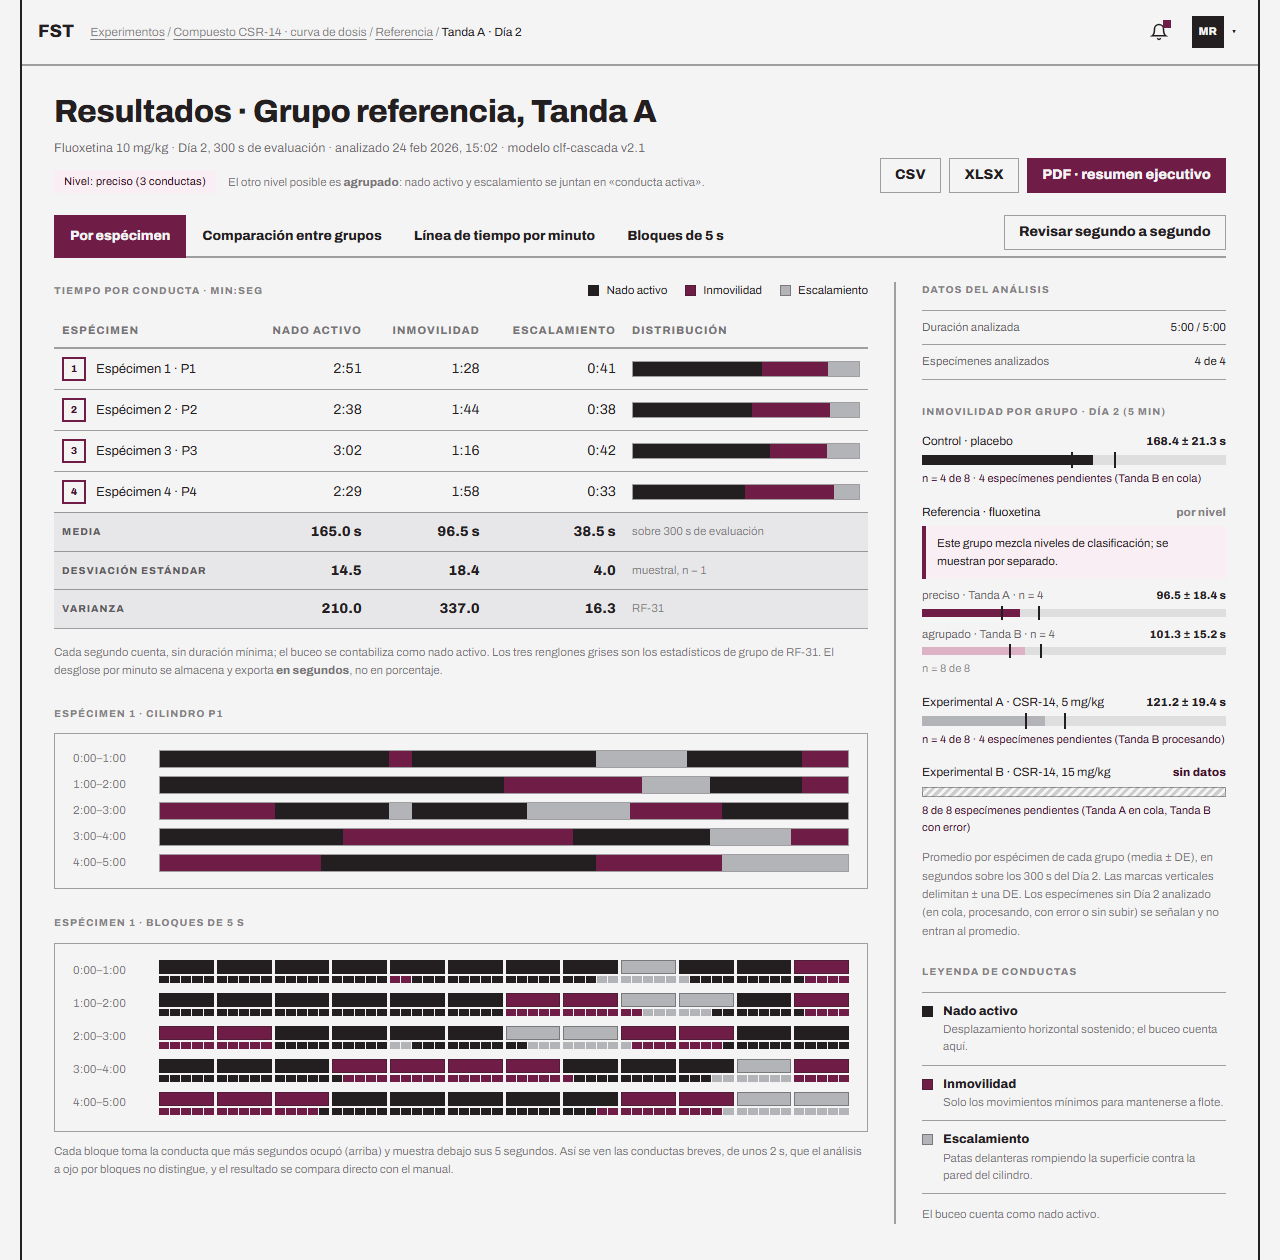
\includegraphics[width=\textwidth]{figures/mockups/v2/resultados}
    \caption{Resultados por espécimen.}
    \label{fig:ui_resultados_especimen}
  \end{subfigure}
  \hspace{0.03\textwidth}
  \begin{subfigure}[t]{0.293\textwidth}
    \centering
    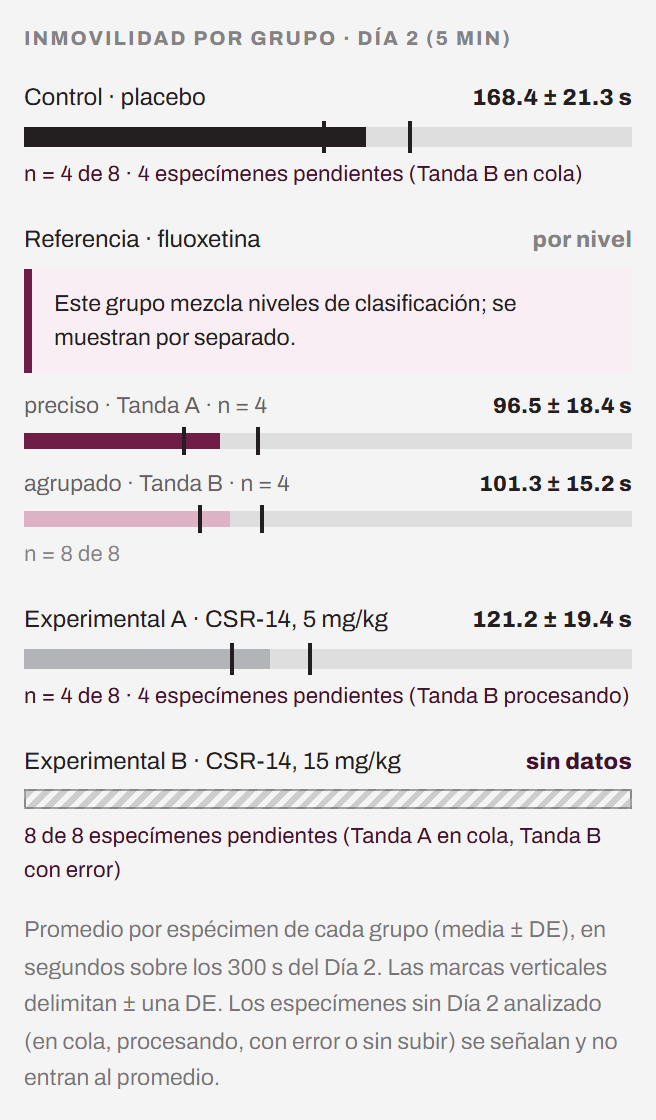
\includegraphics[width=\textwidth]{figures/mockups/v2/estados/resultados_comparacion}
    \caption{Comparación entre grupos en el Día~2 (RF-21).}
    \label{fig:ui_resultados_comparacion}
  \end{subfigure}

  \vspace{8pt}
  \begin{subfigure}[t]{0.75\textwidth}
    \centering
    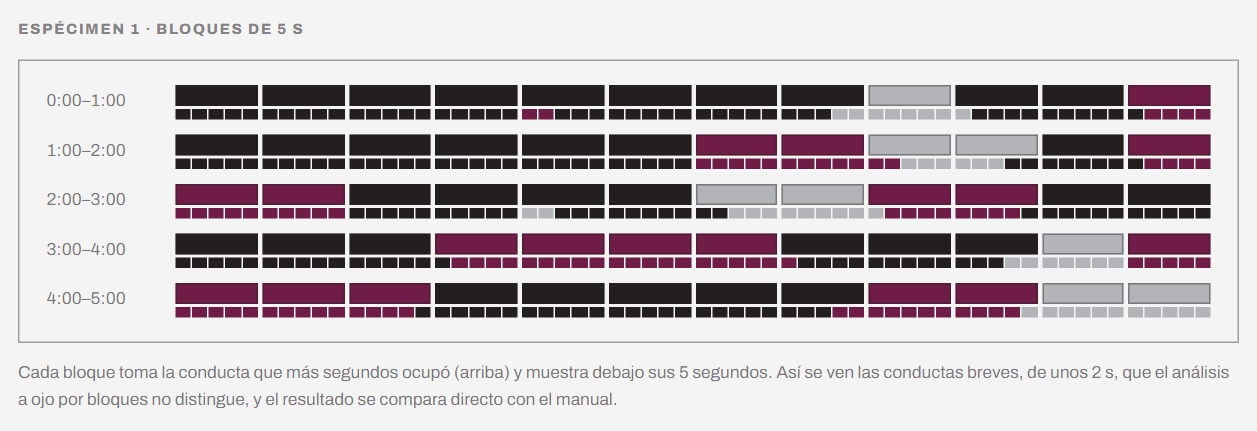
\includegraphics[width=\textwidth]{figures/mockups/v2/estados/resultados_bloques}
    \caption{Bloques de 5~s con sus segundos (RF-18).}
    \label{fig:ui_resultados_bloques}
  \end{subfigure}
\caption{Pantalla de resultados del experimento [autoría propia].}
\label{fig:ui_resultados}
\end{figure}

\subsection{Revisión segundo a segundo}

Se abre solo cuando el análisis está completado, desde la pantalla de progreso o
desde la de resultados (RF-32, RN-14). Muestra el video, con el tubo del espécimen
que se revisa destacado, y una línea de tiempo por espécimen coloreada por
conducta: una vista ampliada de 40~s alrededor del segundo actual y otra de los
300~s completos. Cada segundo ya trae la etiqueta propuesta por el sistema; cuando
no coincide con lo que el usuario observa, pulsa la conducta correcta. Con el video
corriendo, el cambio se aplica desde 0.4~s antes del clic hasta el siguiente cambio
de color; en pausa, cambia solo el segundo actual. Se revisa un espécimen a la vez y
el avance se guarda como borrador en el navegador hasta que el usuario elige
«Guardar», momento en que el sistema registra las correcciones, conserva la
propuesta original y recalcula los totales por minuto (CU-25 a CU-27).

El panel lateral muestra la conducta del segundo actual y si es la propuesta del
sistema o una corrección, el avance de revisión del espécimen, los segundos por
conducta antes y después de corregir, y el nivel de clasificación que tendrá el
análisis al guardar: si algún segundo queda como conducta activa, el análisis pasa a
nivel agrupado (RN-13). A esta pantalla se llega con el botón «Revisar segundo a
segundo» de la pantalla de resultados.

\begin{figure}[H]
\centering
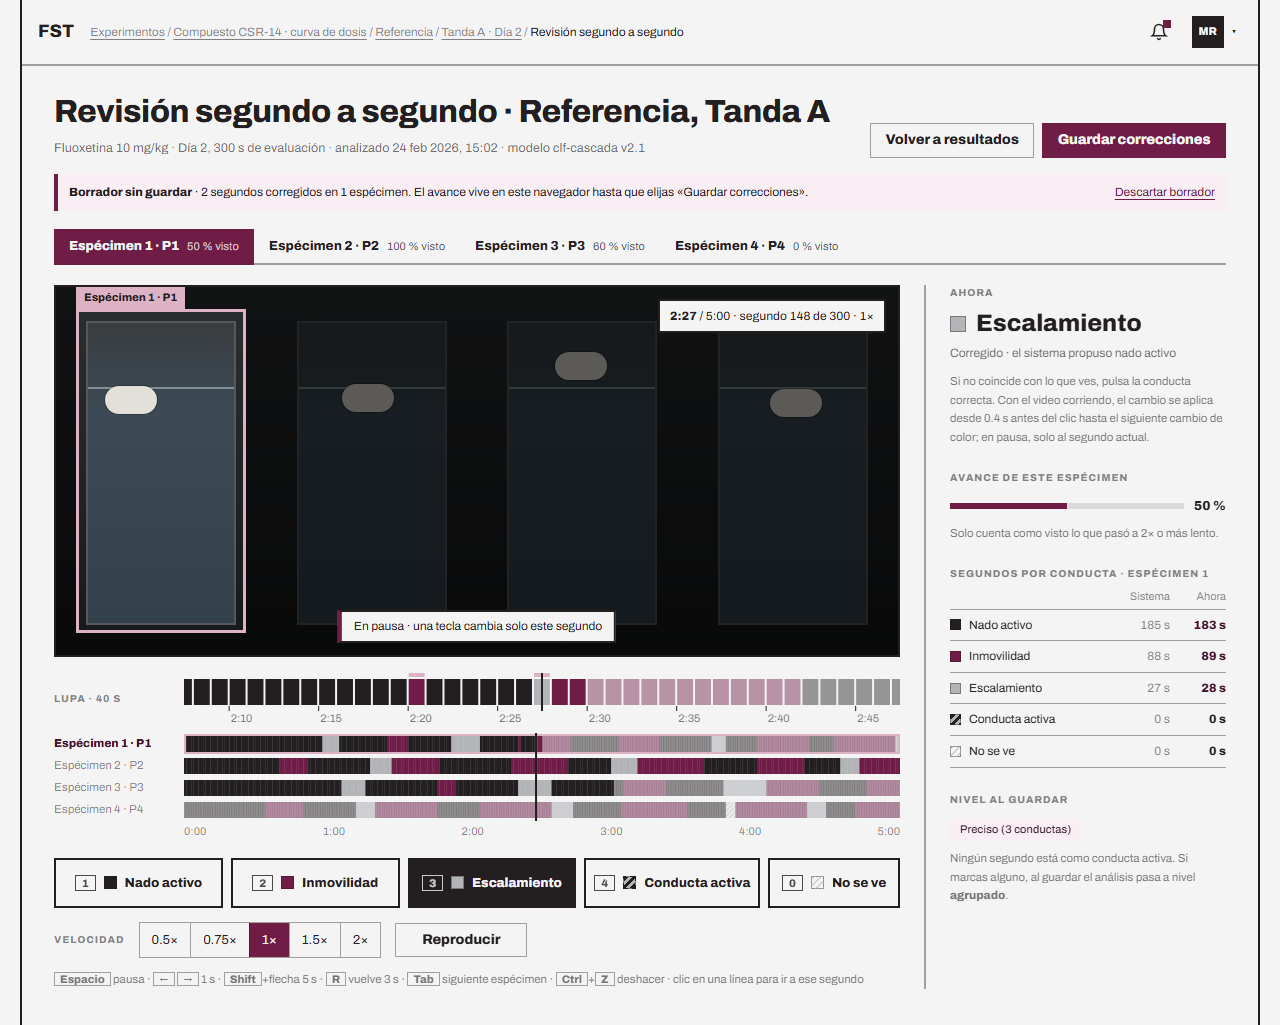
\includegraphics[width=\textwidth]{figures/mockups/v2/revision}
\caption{Pantalla de revisión segundo a segundo [autoría propia].}
\label{fig:ui_revision}
\end{figure}

\subsection{Panel de administración}

Vista exclusiva para quienes pertenecen a \texttt{ADMINISTRADOR} (ver CU-15).
Muestra la lista de cuentas con correo, rol y estado, y permite desactivarlas sin
borrarlas; la cola de trabajos; el uso de almacenamiento, con un aviso al llegar
al 80\,\% de disco y el borrado de los videos más antiguos al llegar al 90\,\% (RF-29,
RNF-09); y las conductas y el modelo del clasificador en uso. Para crear una cuenta, el
Administrador captura identificador institucional, nombre, apellidos y correo (RF-05);
el sistema envía la contraseña temporal por correo y además se la muestra una sola vez
al Administrador, como respaldo.
Al editar una cuenta puede cambiar el nombre, los apellidos, el correo y el estado
(activa o inactiva); el identificador institucional es de solo lectura, y el sistema
impide dejar sin ningún Administrador activo.

\begin{figure}[H]
\centering
  \begin{subfigure}[t]{0.533\textwidth}
    \centering
    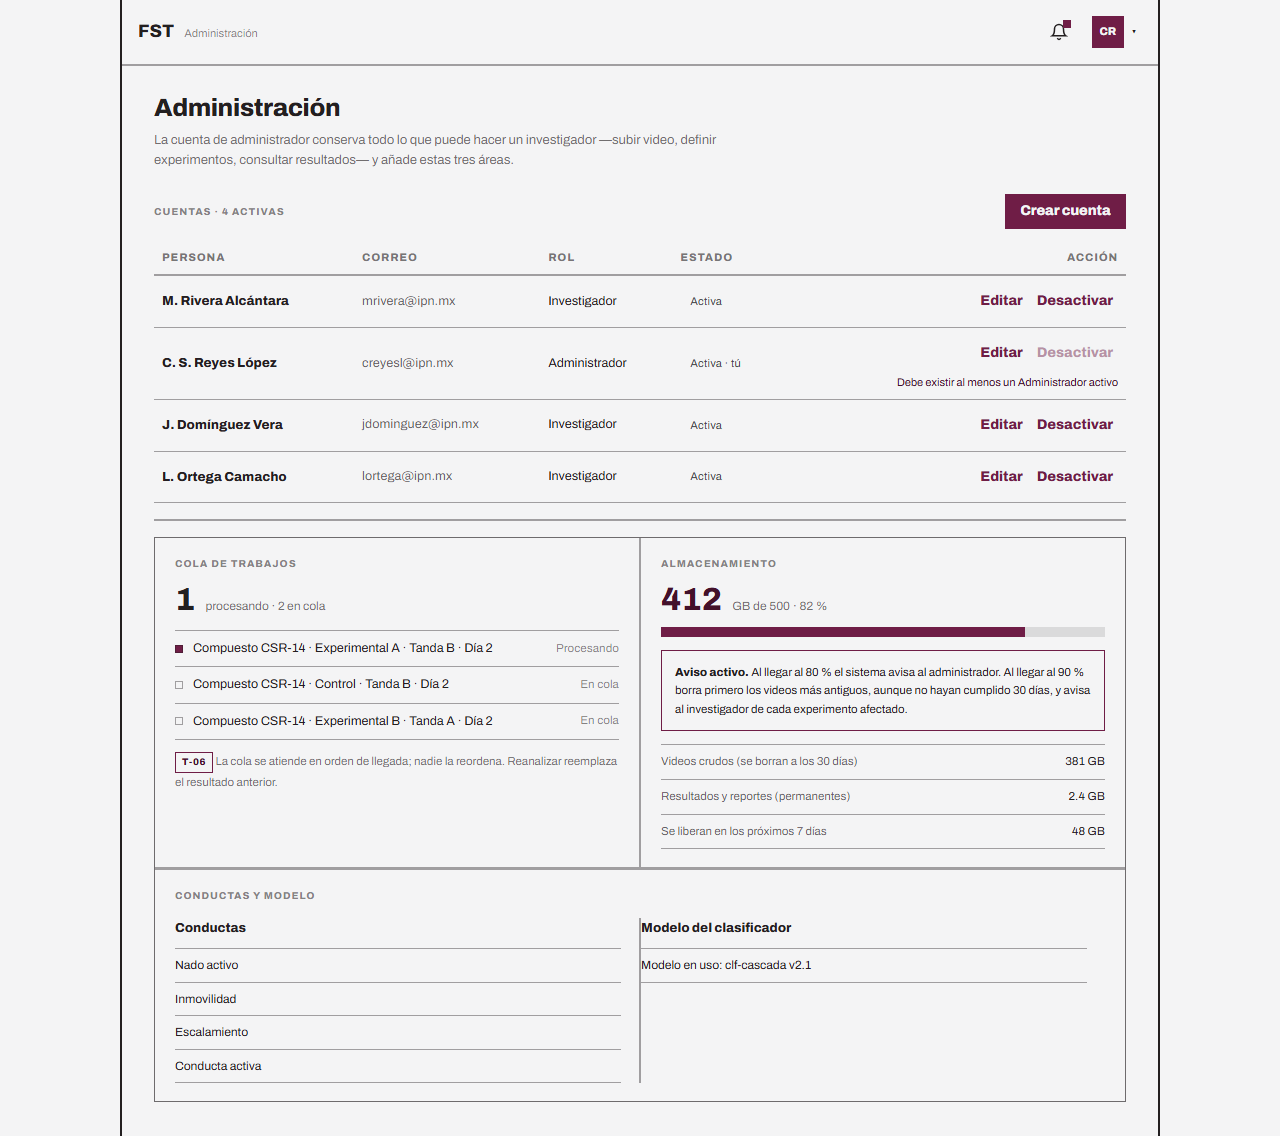
\includegraphics[width=\textwidth]{figures/mockups/v2/admin}
    \caption{Cuentas, cola y almacenamiento.}
    \label{fig:ui_admin_normal}
  \end{subfigure}
  \hfill
  \begin{subfigure}[t]{0.427\textwidth}
    \centering
    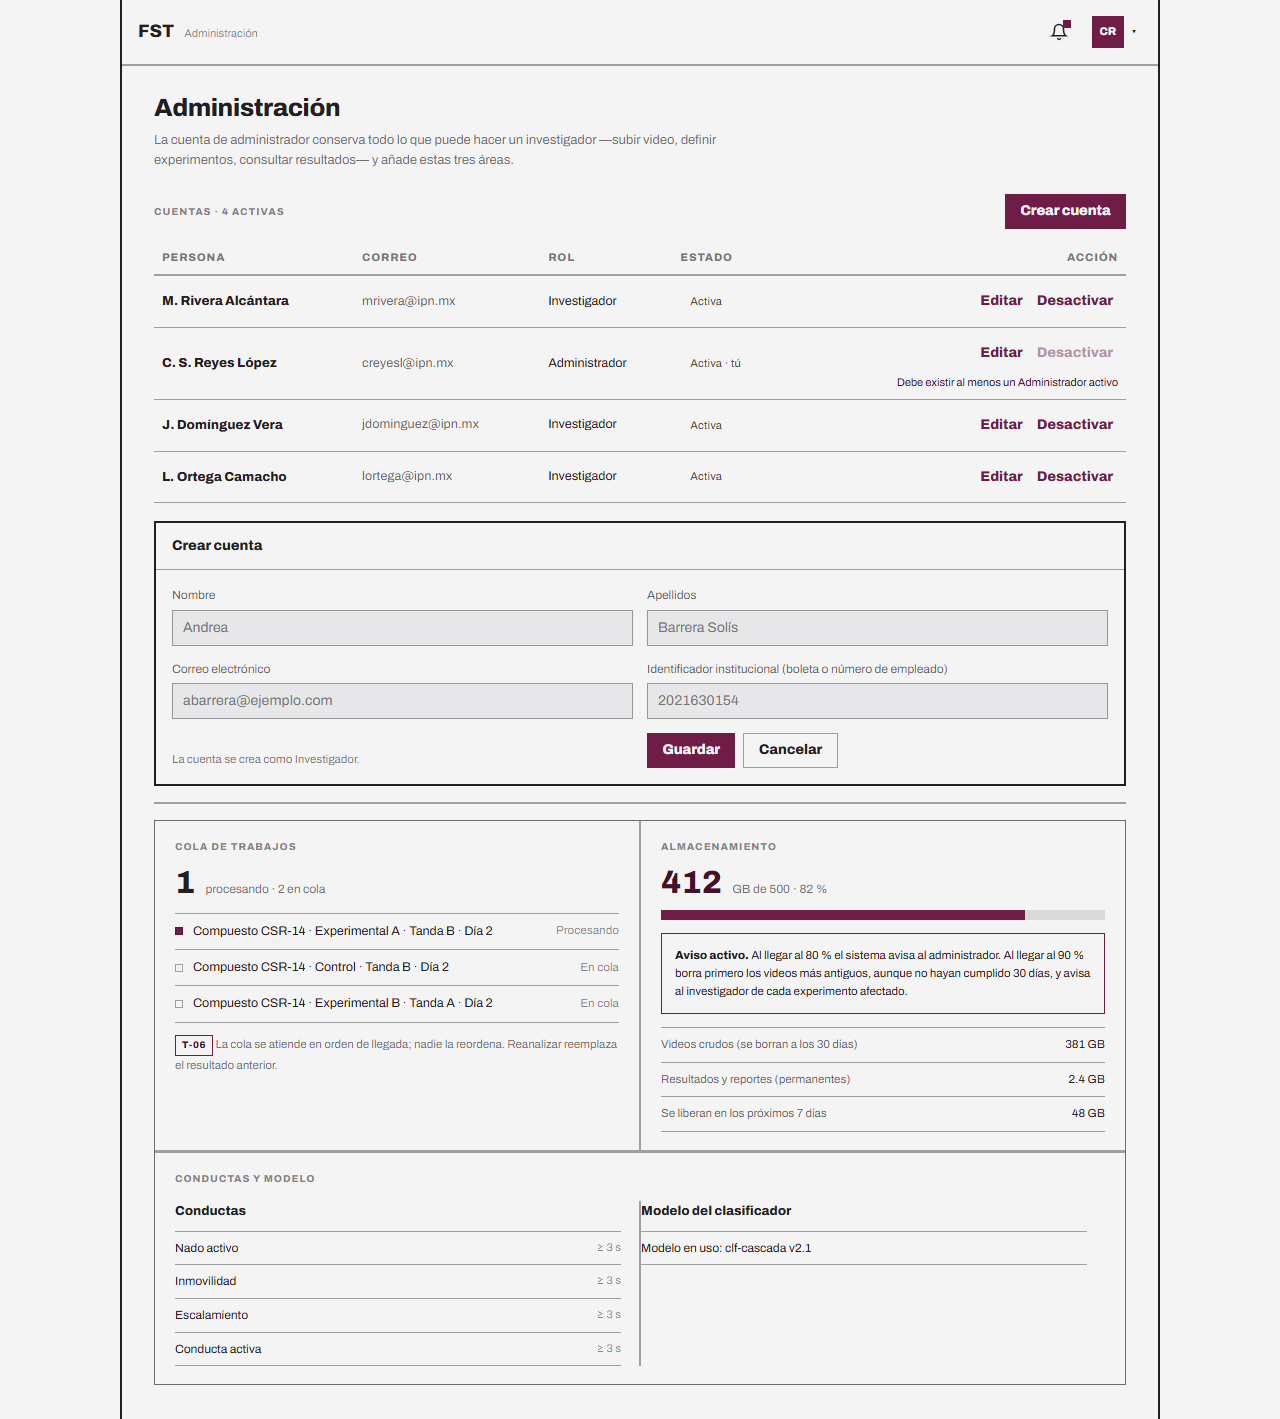
\includegraphics[width=\textwidth]{figures/mockups/v2/estados/admin_crear_cuenta}
    \caption{Formulario de creación de cuenta (RF-05).}
    \label{fig:ui_admin_crear}
  \end{subfigure}

  \vspace{8pt}
  \begin{subfigure}[t]{0.80\textwidth}
    \centering
    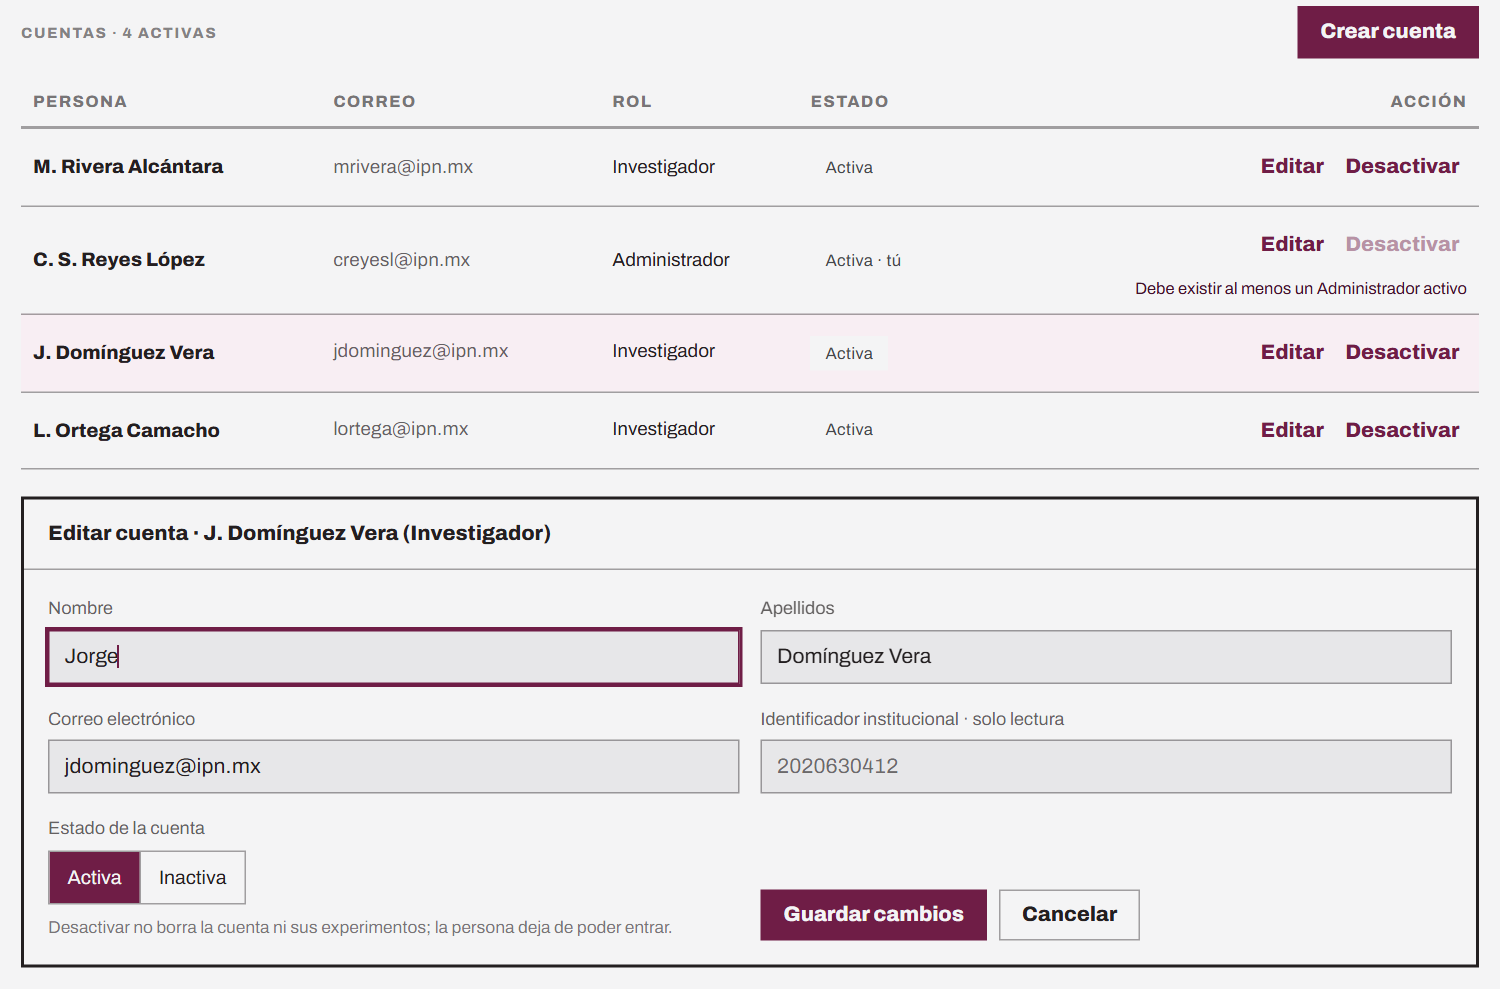
\includegraphics[width=\textwidth]{figures/mockups/v2/estados/admin_editar_cuenta}
    \caption{Edición de una cuenta (RF-05).}
    \label{fig:ui_admin_editar}
  \end{subfigure}
\caption{Panel de administración [autoría propia].}
\label{fig:ui_admin}
\end{figure}
